
\documentclass[10pt,a4paper]{article}

%\usepackage[title,titletoc]{appendix}
%\renewcommand{\appendixname}{Annexe}
%\usepackage{titlesec}

\usepackage{titlesec}
\usepackage{tocloft}
% Largeur réservée aux numéros dans la table des matières

\setlength{\cftsecnumwidth}{7em}
\setlength{\cftsubsecnumwidth}{8em}
\setlength{\cftsubsubsecnumwidth}{10em}
\setlength{\cftparanumwidth}{12em}
\setlength{\cftsubparanumwidth}{14em}

%\setlength{\cftsecnumwidth}{7em}

% Langue et polices
\usepackage[french]{babel}
\usepackage{fontspec}

% Mathématiques
\usepackage{amsmath}
\usepackage{amssymb}
\usepackage{latexsym}

\usepackage{graphicx}  % Insertion des images

% Graphiques et figures
\usepackage{tikz}
\usepackage{graphicx}
\usepackage{caption}
\usepackage{subcaption} % Environnement subfigure
\usepackage{epstopdf}

%\usepackage{placeins}
\usepackage[section]{placeins}

% Couleurs
\usepackage{xcolor}

% Mise en page
%\usepackage{geometry}
%\geometry{margin=22mm}

\usepackage{booktabs}

\pagestyle{plain}

% Espacement entre les lignes
%\renewcommand{\baselinestretch}{1.5}

% Profondeur de la table des matières
\setcounter{tocdepth}{5}
\setcounter{secnumdepth}{5}

% Styles TikZ
\tikzset{
  aretevisible/.style={
    black,
    line width=0.85pt,
    line cap=round
  },
  aretecachee/.style={
    black,
    dashed,
    dash pattern=on 2.4pt off 2pt,
    line width=0.70pt
  }
}

% Commandes mathématiques
\newcommand{\DE}{\displaystyle}

\newcommand{\R}{\mathbb{R}}
\newcommand{\N}{\mathbb{N}}
\newcommand{\Z}{\mathbb{Z}}
\newcommand{\Q}{\mathbb{Q}}
\newcommand{\C}{\mathbb{C}}

% Commandes de couleurs
\newcommand{\RED}[1]{\textcolor{red}{#1}}
\newcommand{\BLUE}[1]{\textcolor{blue}{#1}}
\newcommand{\GREEN}[1]{\textcolor{green!50!black}{#1}}

% Espacement vertical
\newcommand{\esp}{\vspace*{2\bigskipamount}}

\usepackage{hyperref}

% ==================================================
% OPTIMISATION DE L'ESPACE
% ==================================================

% 1. Marges de la page A4
\usepackage[a4paper,
  left=17mm,
  right=17mm,
  top=16mm,
  bottom=18mm,
  headheight=13pt,
  headsep=5mm,
  footskip=9mm
]{geometry}

% 2. Interligne légèrement réduit
\linespread{0.96}

% 3. Espacement des paragraphes
\setlength{\parskip}{0pt}
\setlength{\parindent}{1.2em}

% 4. Espacement entre les sections
\usepackage{titlesec}

\titlespacing*{\section}
  {0pt}{1.5ex plus 0.5ex minus 0.2ex}
  {0.7ex}

\titlespacing*{\subsection}
  {0pt}{1.2ex plus 0.4ex minus 0.2ex}
  {0.5ex}

\titlespacing*{\subsubsection}
  {0pt}{1ex plus 0.3ex minus 0.2ex}
  {0.4ex}

\titlespacing*{\paragraph}
  {0pt}{0.8ex plus 0.2ex minus 0.1ex}
  {0.6em}

% 5. Espacement autour des formules
\AtBeginDocument{
  \setlength{\abovedisplayskip}{6pt plus 2pt minus 2pt}
  \setlength{\belowdisplayskip}{6pt plus 2pt minus 2pt}
  \setlength{\abovedisplayshortskip}{3pt plus 1pt}
  \setlength{\belowdisplayshortskip}{4pt plus 1pt}
}

% 6. Espacement des listes
\usepackage{enumitem}

\setlist{
  topsep=3pt,
  partopsep=0pt,
  itemsep=1pt,
  parsep=0pt
}

% 7. Éviter les blancs verticaux excessifs
\raggedbottom

% 8. Améliorer la composition des paragraphes
\usepackage{microtype}

% ==================================================

%\usepackage{xcolor}

%\newcommand{\RED}[1]{\textcolor{red}{#1}}
%\newcommand{\BLUE}[1]{\textcolor{blue}{#1}}
%\newcommand{\GREEN}[1]{\textcolor{green}{#1}}

\newenvironment{TexteRouge}
  {\begingroup\color{red}}
  {\endgroup}

\newenvironment{TexteBleu}
  {\begingroup\color{blue}}
  {\endgroup}


% ==================================================
% Titre
% ==================================================

\title{
{\Large \sc Albert School}\\
=============\\
{\Large \sc Graph Analytics - Mr. Gianluca Quercini's Teaching}\\
\begin{TexteBleu}
{{\Large \scshape Project} -
{\LARGE Graph Analytics\\of\\Collective Fish Schooling Behaviour}}
\end{TexteBleu}
}

% ==================================================
% Auteurs et adresses e-mail
% ==================================================

\author{
Jacques CHEVOLOT\\
\texttt{jchevolot@albertschool.com}
\and
Charles SCANNAVINO\\
\texttt{cscannavino@albertschool.com}
}

% ==================================================
% Code source et résultats
% ==================================================

\date{
\small
Source code and experimental results:\\
\href{https://github.com/Charles-Scannavino/Projet_Graph_Analytics}
{\texttt{GitHub -- Projet\_Graph\_Analytics}}
}

% ==================================================
% Début du document
% ==================================================

\begin{document}

\maketitle


% ============================================================
% ABSTRACT
% ============================================================

\begin{center}
{\sc Abstract}
\end{center}

{\it This study investigates the structural organisation of a fish
school through the construction and analysis of spatial
proximity graphs. Using empirical observations of individual
positions and velocities, the objective is to examine how
graph-theoretical properties can describe collective cohesion,
fragmentation and local organisation.

The analysis focuses on connectivity, graph distances,
centrality measures and community structure. These
complementary approaches provide a mathematical framework
for describing the relationships between individual
neighbourhoods and the overall configuration of the school.

Two complementary graph representations are considered:
an undirected spatial proximity graph and a directed
visibility graph. Their structural properties are compared
across observation times and neighbourhood radii.

Particular attention is given to the interpretation of the
resulting network measures and to the limitations introduced
by the graph construction process.}

\esp

\begin{center}
{\Large *   *   *}
\end{center}

\tableofcontents

\clearpage

% ============================================================
% 1. INTRODUCTION
% ============================================================

\section{Introduction}

A team of fish, much like a flock of birds, provides a
representative example of collective behaviour in which the
movements of individual agents give rise to coherent patterns
at the group level. The observation of such systems reveals
different forms of spatial organisation, ranging from highly
coordinated motion to local fragmentation, dispersion and
subsequent reaggregation.

The understanding of these collective dynamics requires a
representation capable of describing both the characteristics
of individual fish and the interactions that may occur between
neighbouring individuals. Graph theory provides an appropriate
mathematical framework for this purpose. Each fish can be
represented by a vertex, while edges connect individuals
satisfying a predefined spatial proximity criterion. The
resulting network makes it possible to examine the local
structure of the school and to investigate how individual
neighbourhoods contribute to its overall organisation.

Several hypotheses may be considered to explain the
configurations observed within a fish school. Collective
cohesion may result from a sufficiently dense network of
local interactions; conversely, the disappearance of certain
connections may produce isolated individuals or distinct
connected components. Moreover, the structural position of
individual fish may vary considerably, suggesting differences
in their potential contribution to the connectivity and
organisation of the group.

The present project therefore aims to investigate the extent
to which the topological properties of spatial proximity
graphs can account for the cohesion, fragmentation and
structural organisation of a fish school. The analysis relies
on empirical observations of individual positions and
velocities, from which graphs are constructed and examined
using established methods of network analysis.

Particular attention is given to connectivity, graph
distances, centrality measures and community structure.
These properties provide complementary descriptions of the
network: connectivity characterises the extent to which
individuals belong to a common structure; distances describe
the separation between vertices in terms of successive
connections; centrality measures identify structurally
prominent individuals; and community detection investigates
the existence of relatively cohesive subgroups.

The relevance of these measures will ultimately be assessed
through their confrontation with the observed spatial
configurations of the school. It is important, however, to
distinguish the mathematical properties of a proximity network
from the underlying biological interactions. The presence of
an edge indicates spatial closeness according to the selected
construction rule; it does not, by itself, establish
communication, behavioural influence or a causal relationship
between two fish.

The objective is consequently not only to calculate network
statistics, but also to determine what these statistics
reveal about the organisation of the observed system, while
identifying the limitations introduced by the graph
representation itself.

% ============================================================
% 2. DATASET PRESENTATION
% ============================================================

\section{Dataset Presentation}

\subsection{Description and Source of the Dataset}

The present study is based on an empirical dataset describing
the movements of a school of fish. The data are obtained
from the \textit{Fish Schooling Data Subset}, made available
through Oregon State University.

The dataset contains observations associated with a school
of 300 fish, recorded at a frequency of 30 frames per second
over 5,000 frames. It provides a temporal description of
individual movements through two-dimensional positions and
velocity components.

The principal variables considered in this analysis are
the following:

\begin{itemize}

   \item \textbf{px}: horizontal position of an individual
   fish;

   \item \textbf{py}: vertical position of an individual
   fish;

   \item \textbf{vx}: horizontal component of its velocity;

   \item \textbf{vy}: vertical component of its velocity;

   \item \textbf{onfish}: field used as an individual
   tracking identifier in the project implementation.

\end{itemize}

These variables make it possible to reconstruct the spatial
configuration of the school at successive observation times
and to investigate the evolution of its local neighbourhood
structure.

The data are stored in JSON format. Their temporal
organisation allows the analysis of individual frames as
well as comparisons between distinct observation periods.

\subsection{Representation of the Fish School as a Graph}

The empirical observations are not initially provided as a
network. A graph representation must therefore be constructed
from the recorded positions of the individuals.

Let $G_t=(V_t,E_t)$ denote the graph associated with an
observation frame $t$, where $V_t$ represents the set of fish
included in the analysis and $E_t$ the set of connections
established between neighbouring individuals.

Each vertex $i \in V_t$ is associated with a position vector

\begin{equation}
X_i(t)=
\begin{pmatrix}
x_i(t)\\
y_i(t)
\end{pmatrix}
\in \mathbb{R}^{2},
\end{equation}

and a velocity vector

\begin{equation}
V_i(t)=
\begin{pmatrix}
v_{x,i}(t)\\
v_{y,i}(t)
\end{pmatrix}.
\end{equation}

The spatial separation between two individuals $i$ and $j$
is defined by the Euclidean distance

\begin{equation}
d_{ij}(t)=
\sqrt{
\left(x_i(t)-x_j(t)\right)^2+
\left(y_i(t)-y_j(t)\right)^2
}.
\end{equation}

A connection is introduced whenever this distance satisfies
a predefined proximity criterion:

\begin{equation}
(i,j)\in E_t
\quad\Longleftrightarrow\quad
i\neq j
\quad \text{and} \quad
d_{ij}(t)<R,
\end{equation}

where $R>0$ denotes the neighbourhood radius.

This construction produces an undirected, simple graph,
provided that the proximity criterion is applied
symmetrically and that each pair of fish is connected
by at most one edge.

The number of vertices is denoted by

\begin{equation}
N_t=|V_t|,
\end{equation}

while the number of edges is given by

\begin{equation}
M_t=|E_t|.
\end{equation}

Although the original dataset describes a school of 300 fish,
the effective number of vertices in a particular frame must
be determined from the valid observations retained during
graph construction.

The resulting network provides a representation of spatial
proximity rather than a direct measurement of social or
behavioural interactions. Its structure consequently depends
on the selected radius, the distribution of fish positions
and the completeness of the available observations.

\subsection{Interpretation of the Graph Representation}

The construction of a proximity graph makes it possible to
move from the individual description of fish trajectories
to the analysis of collective organisation.

A fish situated within a densely occupied region may be
connected to numerous neighbours, whereas an individual
located at the periphery of the school may have relatively
few connections. Similarly, spatially separated groups may
form distinct connected components, reflecting a
fragmentation of the network under the selected proximity
criterion.

The choice of the neighbourhood radius is therefore of
particular importance. A small radius may produce a sparse
and fragmented graph, while a larger radius may connect
previously separated groups and increase the overall
density of the network.

The subsequent analysis examines these structural
properties using graph-theoretical measures, with particular
attention to the interpretation of their variations and
their dependence on the graph construction parameters.

% ============================================================
% 3. DESCRIPTION OF THE ANALYSIS
% ============================================================

\section{Description of the Analysis}

\subsection{Analytical Framework and Software}

The analysis of the fish school relies on the construction
of graphs representing the relationships between individuals
at a given observation time.

Two complementary models have been implemented. The first
is based exclusively on the spatial proximity of the fish,
while the second introduces a directional visibility
constraint derived from their velocity vectors.

The objective is to examine the extent to which these
representations make it possible to describe the
connectivity, cohesion and internal organisation of the
school.

The numerical analysis has been developed in Python,
using the NetworkX library for graph construction and
the calculation of network measures. NumPy and SciPy
are used for numerical operations and Euclidean distance
calculations, while Matplotlib provides the graphical
representations of the results.

The experimental data are read from the JSON dataset
using the ijson library, which allows individual frames
to be extracted without loading the entire dataset
into memory.

The principal methods are described below.

\subsection{Construction of the Spatial Proximity Graph}

The first model considers an undirected graph in which
each vertex represents an individual fish and each edge
corresponds to a spatial neighbourhood relationship.

For two distinct individuals $i$ and $j$, the adjacency
matrix is defined by

\begin{equation}
A_{ij}(t)=
\begin{cases}
1, & \text{if } d_{ij}(t)<R,\\
0, & \text{otherwise},
\end{cases}
\qquad i\neq j,
\end{equation}

with

\begin{equation}
A_{ii}(t)=0.
\end{equation}

The parameter $R$ denotes the neighbourhood radius.

Since the Euclidean distance is symmetric, the resulting
adjacency matrix satisfies

\begin{equation}
A_{ij}(t)=A_{ji}(t).
\end{equation}

The graph is therefore undirected. It is also simple,
since self-loops and multiple edges are excluded.

Each edge retains the Euclidean distance between the
corresponding individuals as an attribute. However,
the structural measures presented in this study are
calculated without using these distances as weights.

All detected fish are retained as vertices, including
those having no neighbours within the selected radius.

The reference value is set to

\begin{equation}
R=100,
\end{equation}

expressed in the native coordinate units of the dataset.

This value is used as a descriptive reference rather
than as a biologically validated interaction distance.

Additional analyses are performed for

\begin{equation}
R\in\{60,80,100,120,140\},
\end{equation}

in order to examine the sensitivity of the network
properties to the selected spatial threshold.

\subsection{Construction of the Directed Visibility Graph}

The second model introduces an additional condition
associated with the direction of movement of each fish.

Unlike the spatial graph, the visibility graph is
directed. An arc from individual $i$ to individual $j$
exists when the two fish satisfy the proximity condition
and when $j$ lies outside the rear blind sector of $i$.

The direction of movement is approximated by

\begin{equation}
\theta_i(t)=
\operatorname{atan2}
\left(v_{y,i}(t),v_{x,i}(t)\right).
\end{equation}

The direction from individual $i$ towards individual
$j$ is given by

\begin{equation}
\phi_{ij}(t)=
\operatorname{atan2}
\left(
y_j(t)-y_i(t),
x_j(t)-x_i(t)
\right).
\end{equation}

The angular difference is calculated using

\begin{equation}
\Delta\theta_{ij}(t)=
\operatorname{atan2}
\left(
\sin(\phi_{ij}-\theta_i),
\cos(\phi_{ij}-\theta_i)
\right).
\end{equation}

A directed connection is introduced if

\begin{equation}
d_{ij}(t)<R
\end{equation}

and

\begin{equation}
|\Delta\theta_{ij}(t)|
\leq
\pi-\frac{\alpha}{2},
\end{equation}

where $\alpha$ denotes the total angular width
of the rear blind sector.

In the present implementation,

\begin{equation}
\alpha=25^{\circ}.
\end{equation}

The nominal field of visibility therefore covers
$335^{\circ}$.

The resulting graph is directed because the visibility
condition is not necessarily symmetric:

\begin{equation}
A_{ij}(t)\neq A_{ji}(t)
\end{equation}

for some pairs of individuals.

A fish may consequently be able to perceive another
individual without the reciprocal condition being
satisfied.

This representation remains a geometrical approximation.
The velocity vector is used as a proxy for orientation;
the model does not directly measure the visual perception
or attention of the animals.

\subsection{Connectivity and Connected Components}

The connectivity of a graph provides a first indication
of its global organisation.

For the undirected spatial graph, two vertices are
connected if a path exists between them.

A connected component is a maximal subset of vertices
within which every pair of individuals can be joined
by a sequence of edges.

The number of connected components is denoted by

\begin{equation}
C(G).
\end{equation}

The relative size of the largest connected component
is calculated as

\begin{equation}
S_{\mathrm{LCC}}=
\frac{|V_{\mathrm{LCC}}|}{|V|}.
\end{equation}

This quantity measures the proportion of observed
individuals belonging to the largest connected
structure.

For the directed visibility graph, two distinct
definitions are considered:

\begin{itemize}

\item \textbf{Weak connectivity}: connectivity obtained
when the direction of the arcs is ignored;

\item \textbf{Strong connectivity}: connectivity for
which every vertex can reach every other vertex
through directed paths.

\end{itemize}

These definitions are not interchangeable and must
be distinguished when comparing the two graph models.

\subsection{Graph Density and Degree Distribution}

The degree of a vertex $i$ in the undirected graph
corresponds to the number of neighbouring fish
connected to that individual:

\begin{equation}
k_i=\sum_{j=1}^{N}A_{ij}.
\end{equation}

The average degree is defined by

\begin{equation}
\langle k\rangle=\frac{2M}{N},
\end{equation}

where $N$ is the number of vertices and $M$ the
number of edges.

The density of an undirected simple graph is

\begin{equation}
D(G)=\frac{2M}{N(N-1)}.
\end{equation}

For a directed graph without self-loops, the density
is instead defined as

\begin{equation}
D_{\mathrm{dir}}(G)=
\frac{M_{\mathrm{dir}}}{N(N-1)},
\end{equation}

where $M_{\mathrm{dir}}$ denotes the number of arcs.

These indicators provide a description of the
relative abundance of connections within the school.

However, their interpretation must take into account
the number of observed individuals and the selected
neighbourhood radius.

\subsection{Graph Distances, Diameter and Radius}

The distance between two vertices is defined as the
length of the shortest path connecting them.

In the present analysis, the path length is expressed
in numbers of edges, or hops, rather than in physical
distance units.

Let

\begin{equation}
d_G(i,j)
\end{equation}

denote the shortest-path distance between vertices
$i$ and $j$.

The eccentricity of a vertex is defined as

\begin{equation}
e(i)=\max_{j\in V}d_G(i,j).
\end{equation}

The diameter of a connected graph is then

\begin{equation}
\operatorname{diam}(G)=
\max_{i\in V}e(i),
\end{equation}

while its radius is

\begin{equation}
\operatorname{rad}(G)=
\min_{i\in V}e(i).
\end{equation}

Since the observed networks may contain several
components, these measures cannot be interpreted
without specifying the connected subgraph considered.

For the spatial model, the diameter and radius are
calculated on the largest connected component.

For the directed visibility model, they are calculated
on the largest strongly connected component.

This convention avoids assigning finite distances
between vertices for which no path exists.

\subsection{Centrality Measures}

Centrality measures are used to identify individuals
occupying structurally prominent positions within
the network.

Two measures are retained in the principal analysis.

\subsubsection{Degree Centrality}

For an undirected graph, degree centrality is defined
by

\begin{equation}
C_D(i)=\frac{k_i}{N-1}.
\end{equation}

It expresses the proportion of other individuals
directly connected to vertex $i$.

A high degree centrality may indicate that a fish
is situated in a locally dense region of the school.

For the directed visibility graph, in-degree and
out-degree centralities are distinguished.

The out-degree counts the individuals towards which
a fish has an outgoing visibility connection, whereas
the in-degree counts the incoming visibility
connections.

\subsubsection{Betweenness Centrality}

Betweenness centrality measures the extent to which
a vertex belongs to shortest paths connecting other
vertices.

It is defined by

\begin{equation}
C_B(i)=
\sum_{\substack{s\neq i\neq t\\s\neq t}}
\frac{\sigma_{st}(i)}{\sigma_{st}},
\end{equation}

where $\sigma_{st}$ is the number of shortest paths
between vertices $s$ and $t$, and $\sigma_{st}(i)$
the number of those paths passing through vertex $i$.

The values are normalised using the convention
implemented in NetworkX.

An individual with high betweenness centrality may
occupy a position connecting different regions of
the graph.

However, such a position does not establish that
the individual controls the movements of the school
or acts as a biological leader.

\subsection{Clustering Coefficient}

The clustering coefficient describes the tendency
of neighbouring vertices to be connected to one
another.

For an undirected graph, the local clustering
coefficient of vertex $i$ is

\begin{equation}
C_i=
\frac{2T_i}{k_i(k_i-1)},
\end{equation}

where $T_i$ denotes the number of triangles
containing vertex $i$.

The average clustering coefficient is

\begin{equation}
\overline{C}=
\frac{1}{N}\sum_{i=1}^{N}C_i.
\end{equation}

A relatively high clustering coefficient indicates
that neighbouring fish frequently belong to
interconnected local groups.

For directed graphs, the NetworkX implementation
uses a corresponding definition adapted to the
orientation of the arcs.
\subsection{Community Detection}

The identification of communities provides an
additional description of the internal organisation
of the fish school.

A community is understood here as a subset of
vertices having relatively dense internal connections
compared with their connections to other subsets.

Community detection is performed using the Louvain
algorithm, as implemented in NetworkX. The algorithm
seeks a partition associated with relatively high
modularity.

\paragraph{Modularity of the undirected spatial graph.}

For the undirected spatial proximity graph,
modularity is defined as

\begin{equation}
Q_{\mathrm{undirected}}
=
\frac{1}{2M}
\sum_{i,j}
\left(
A_{ij}
-
\frac{k_i k_j}{2M}
\right)
\delta(c_i,c_j),
\end{equation}

where $A_{ij}$ is the adjacency matrix,
$k_i$ and $k_j$ are the degrees of vertices
$i$ and $j$, and $M$ is the number of
undirected edges.

The term $\delta(c_i,c_j)$ equals one when
vertices $i$ and $j$ belong to the same
community, and zero otherwise.

\paragraph{Modularity of the directed visibility graph.}

The visibility graph is directed because the
visibility relationship between two fish is
not necessarily reciprocal.

Louvain community detection is applied directly
to this directed graph, without converting it
into an undirected representation.

For a directed graph, modularity is defined as

\begin{equation}
Q_{\mathrm{directed}}
=
\frac{1}{M}
\sum_{i,j}
\left(
A_{ij}
-
\frac{k_i^{\mathrm{out}}
     k_j^{\mathrm{in}}}{M}
\right)
\delta(c_i,c_j),
\end{equation}

where $M$ is the total number of directed arcs,
$k_i^{\mathrm{out}}$ is the out-degree of vertex
$i$, and $k_j^{\mathrm{in}}$ is the in-degree
of vertex $j$.

This formulation accounts for the orientation
of interactions and is consistent with the
directed modularity implemented in NetworkX.

\paragraph{Implementation and parameters.}

Both graph models are analysed using the
following parameters:

\begin{itemize}
   \item Algorithm: Louvain (NetworkX);
   \item Random seed: $42$;
   \item Resolution parameter: $1.0$;
   \item Edge weights: not used;
   \item Spatial graph: undirected;
   \item Visibility graph: directed.
\end{itemize}

The resulting partitions are evaluated using
the number of detected communities, their sizes,
and the corresponding modularity.

For the first experimental frame, the spatial
graph produces 11 communities with a modularity
of $0.70344$, while the directed visibility
graph produces 10 communities with a modularity
of $0.70500$.

These results are consistent with the outputs
stored in the project repository.

Although both modularity values are numerically
close, they are calculated using different
null models. Their comparison must therefore
be interpreted with caution.

Furthermore, communities identified in spatial
proximity graphs may arise partly from their
geometrical construction.

They must not automatically be interpreted
as stable biological groups or as evidence
of coordinated decision-making.


\subsection{Temporal Analysis and Sensitivity}

The dataset contains 5,000 observation frames,
recorded at 30 frames per second.

In order to investigate variations in network
organisation, a systematic sample of 21 frames
is considered:

\begin{equation}
t\in
\{1,251,501,\ldots,4751,5000\}.
\end{equation}

The corresponding observations cover approximately
166.63 seconds.

For each selected frame, the two graph models
are constructed and their principal structural
properties are calculated.

The analysis is repeated for five neighbourhood
radii:

\begin{equation}
R\in\{60,80,100,120,140\}.
\end{equation}

This approach makes it possible to distinguish
variations associated with the observed spatial
configurations from those introduced by the
graph construction threshold.

The results are summarised using descriptive
statistics and graphical representations.

The temporal curves connect sampled observations;
they do not establish the behaviour of the network
between successive sampled frames.

% ============================================================
% 4. RESULTS
% ============================================================

\section{Results}

\subsection{Structural Properties of the First Frame}

The first analysis is performed on frame 1,
using a neighbourhood radius of $R=100$.

The experimental data contain 253 detected fish
at this observation time.

The spatial graph contains 1,281 undirected edges,
while the directed visibility graph contains
2,386 arcs.

The principal results are presented in
Table~\ref{tab:structural_results}.

\begin{table}[htbp]
\centering
\caption{Structural properties of the two graph models
at frame 1, for $R=100$.}
\label{tab:structural_results}

\small
\begin{tabular}{lcc}
\hline
\textbf{Measure}
& \textbf{Spatial}
& \textbf{Visibility}\\
\hline
Vertices & 253 & 253\\
Edges / arcs & 1,281 & 2,386\\
Relevant components & 4 & 4\\
Largest component & 248 & 248\\
Largest component share & 98.02\% & 98.02\%\\
Diameter (hops) & 23 & 24\\
Radius (hops) & 12 & 12\\
Density & 0.04018 & 0.03742\\
Average clustering & 0.57800 & 0.54551\\
Louvain communities & 11 & 10\\
Modularity & 0.70344 & 0.70500\\
\hline
\end{tabular}
\end{table}

The spatial graph contains four connected components,
with the largest component comprising 248 of the
253 observed individuals.

This corresponds to approximately 98.02\% of the
vertices.

The results therefore indicate that most of the
observed fish belong to a common connected
structure under the selected proximity criterion.

Nevertheless, the existence of four components
shows that the graph is not entirely connected.

The diameter of the largest spatial component
is 23 hops, while its radius is 12 hops.

These values describe the shortest-path structure
of the network and should not be confused with
the Euclidean distances between fish.

The directed visibility graph presents a comparable
global structure, although the directional
constraint modifies the number and orientation
of the available connections.

Its largest strongly connected component contains
248 vertices, with a diameter of 24 hops
and a radius of 12 hops.

\subsection{Centrality and Structural Positions}

The degree and betweenness centralities reveal
differences in the structural positions of
individual fish.

In the spatial graph, the highest degree
centrality is associated with fish identifier
100230, with a normalised score of 0.09921.

The highest betweenness centrality is observed
for fish identifier 99458, with a score
of 0.16501.

These two individuals do not occupy the same
position in the centrality rankings.

This distinction illustrates the complementary
interpretations provided by the two measures.

A fish may be connected to numerous immediate
neighbours without necessarily occupying a
position through which a large proportion of
shortest paths passes.

Conversely, an individual may connect different
regions of the graph while having a more
moderate number of direct neighbours.

For the visibility graph, the highest
betweenness centrality is associated with
identifier 99981, with a score of 0.14945.

The introduction of directional visibility
therefore modifies the ranking of structurally
prominent individuals.

These observations concern network positions
only. They do not demonstrate the existence
of behavioural leadership.

\
\subsection{Community Structure}
\label{subsec:community_structure}

Community detection provides a complementary perspective
on the internal organisation of the fish school. While
connectivity measures establish whether individuals can
be connected through paths, community detection seeks
to identify groups of vertices exhibiting comparatively
dense internal connections.

The Louvain algorithm was used to identify community
partitions in the spatial and visibility networks.
For the first experimental frame, the spatial graph
contains 253 observed fish and 1,281 undirected edges,
whereas the visibility graph contains the same
253 individuals and 2,386 directed arcs.

The resulting partitions exhibit substantial modularity.
The spatial graph contains 11 detected communities,
with a modularity of

\begin{equation}
Q_{\mathrm{spatial}} = 0.70344.
\end{equation}

The visibility graph contains 10 communities, with

\begin{equation}
Q_{\mathrm{visibility}} = 0.70500.
\end{equation}

The largest community of the spatial graph contains
64 individuals, followed by a second community
containing 47 fish. In the visibility graph,
the two largest communities contain 65 and
43 individuals, respectively.

Figure~\ref{fig:community_comparison} illustrates
the geographical distribution of these partitions.

\begin{figure}[htbp]
    \centering

    \begin{subfigure}[t]{0.49\textwidth}
        \centering
        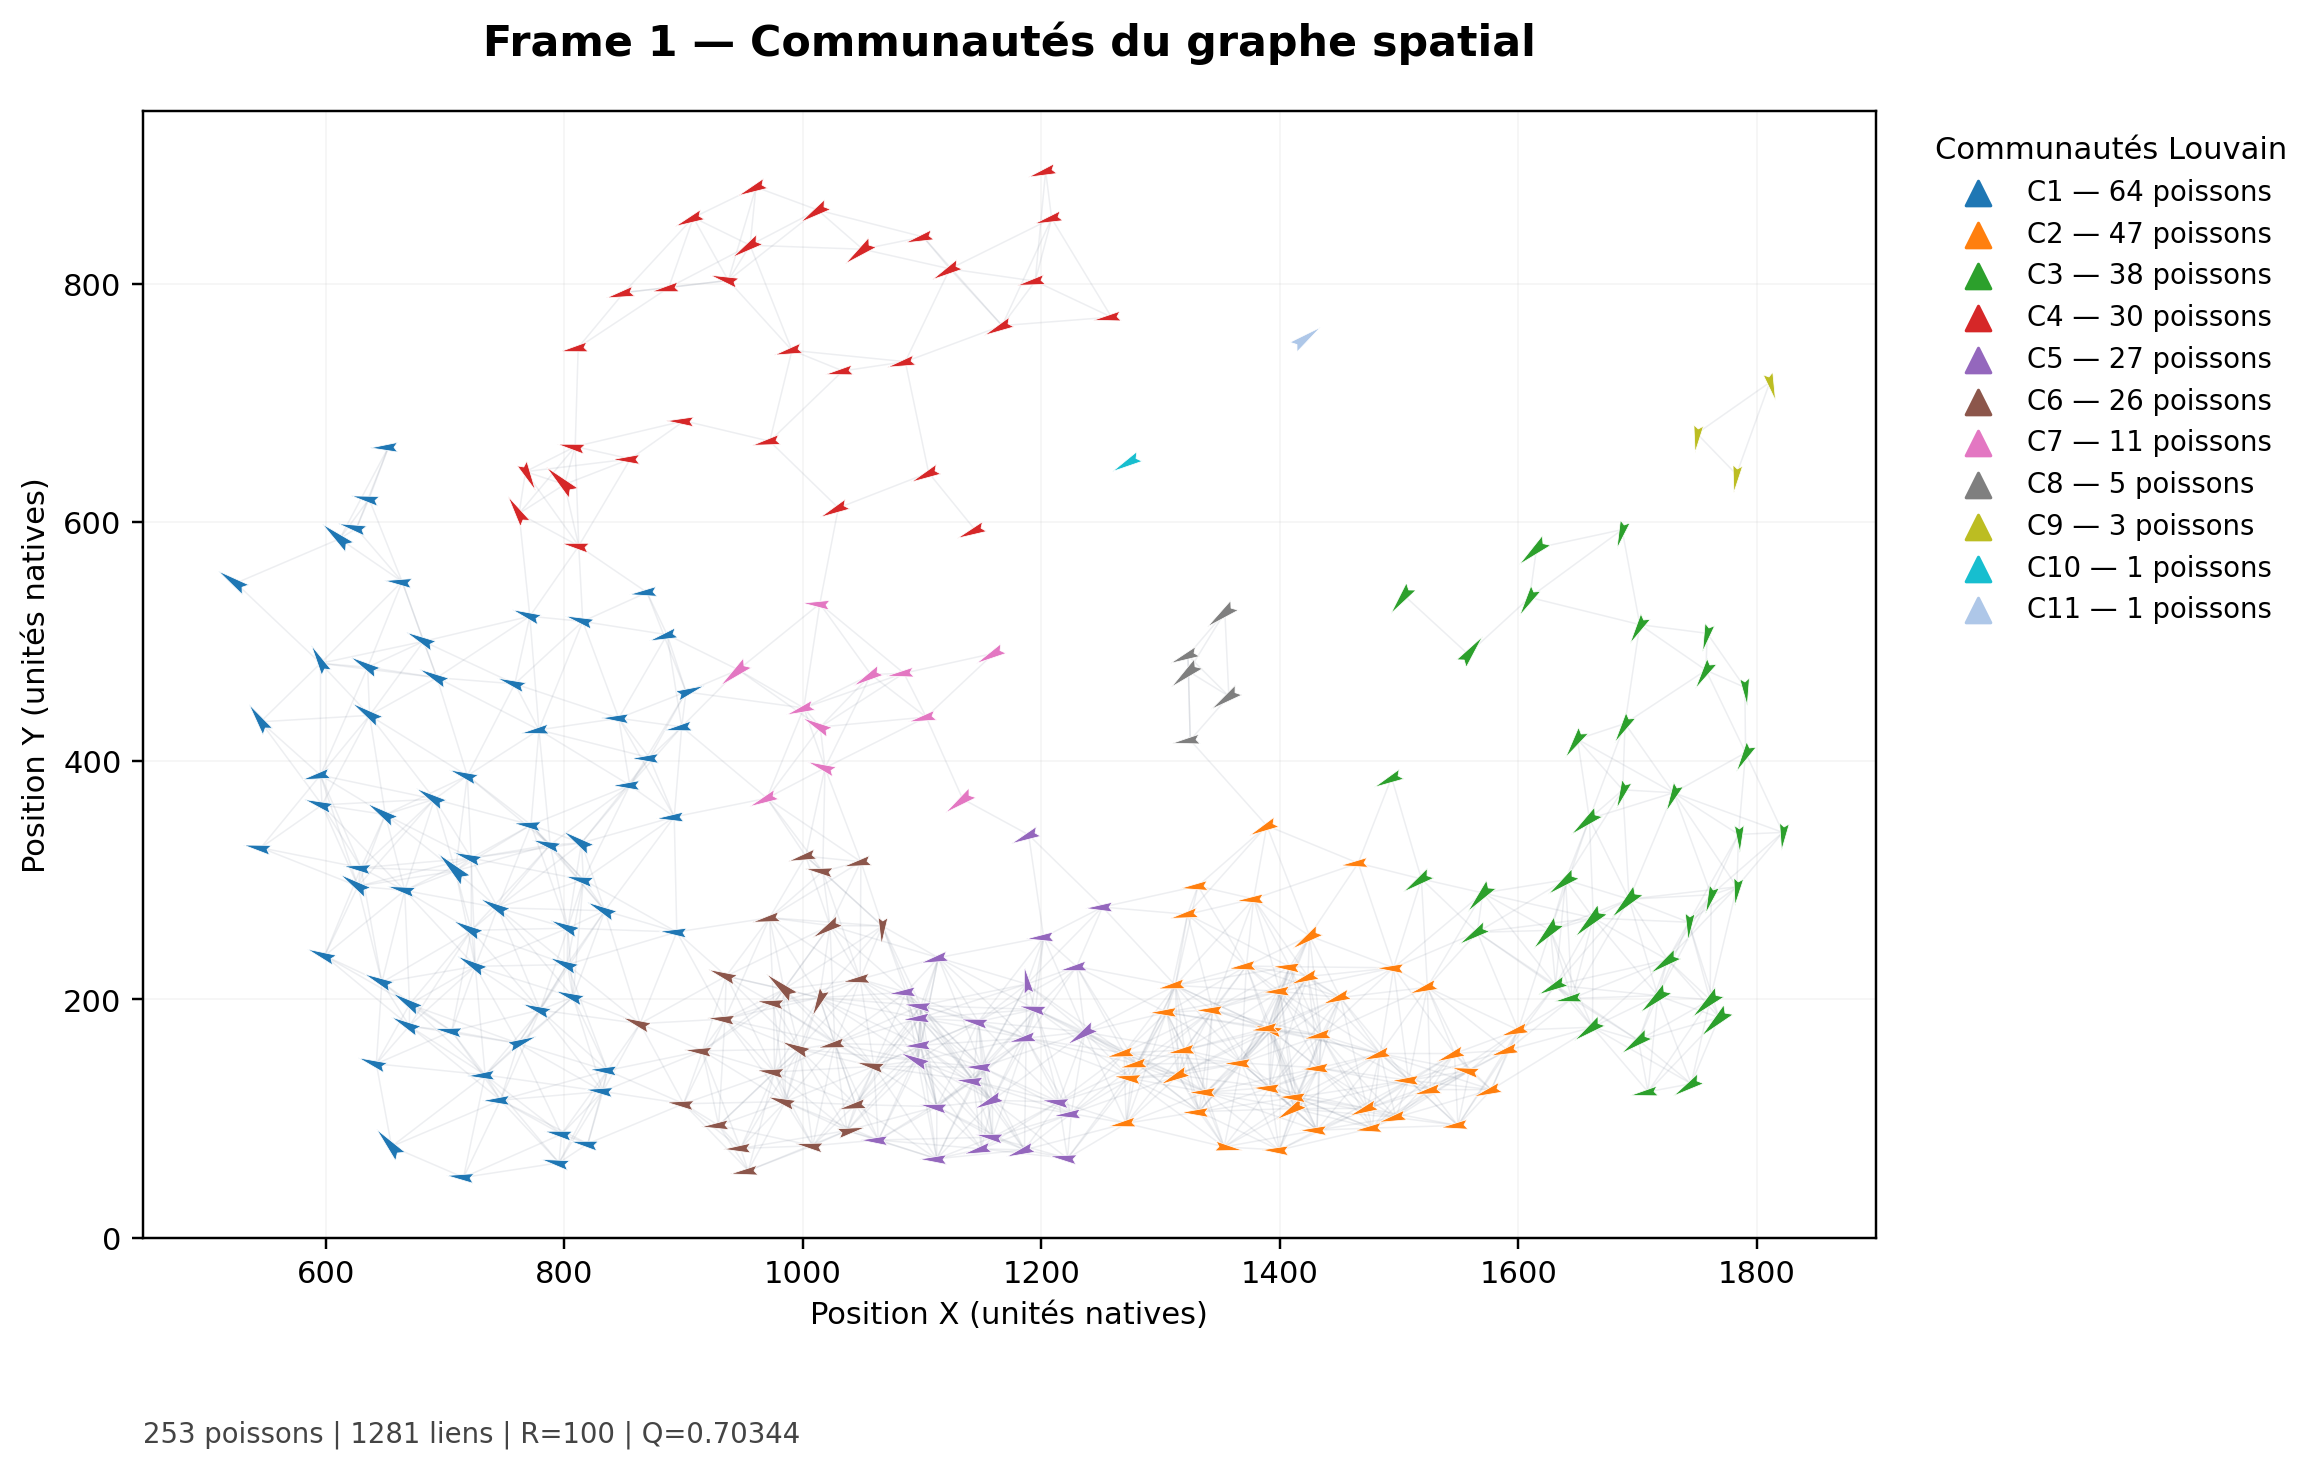
\includegraphics[width=\linewidth]
        {frame1_spatial_louvain.png}
        \caption{Spatial proximity network.}
        \label{fig:spatial_communities}
    \end{subfigure}
    \hfill
    \begin{subfigure}[t]{0.49\textwidth}
        \centering
        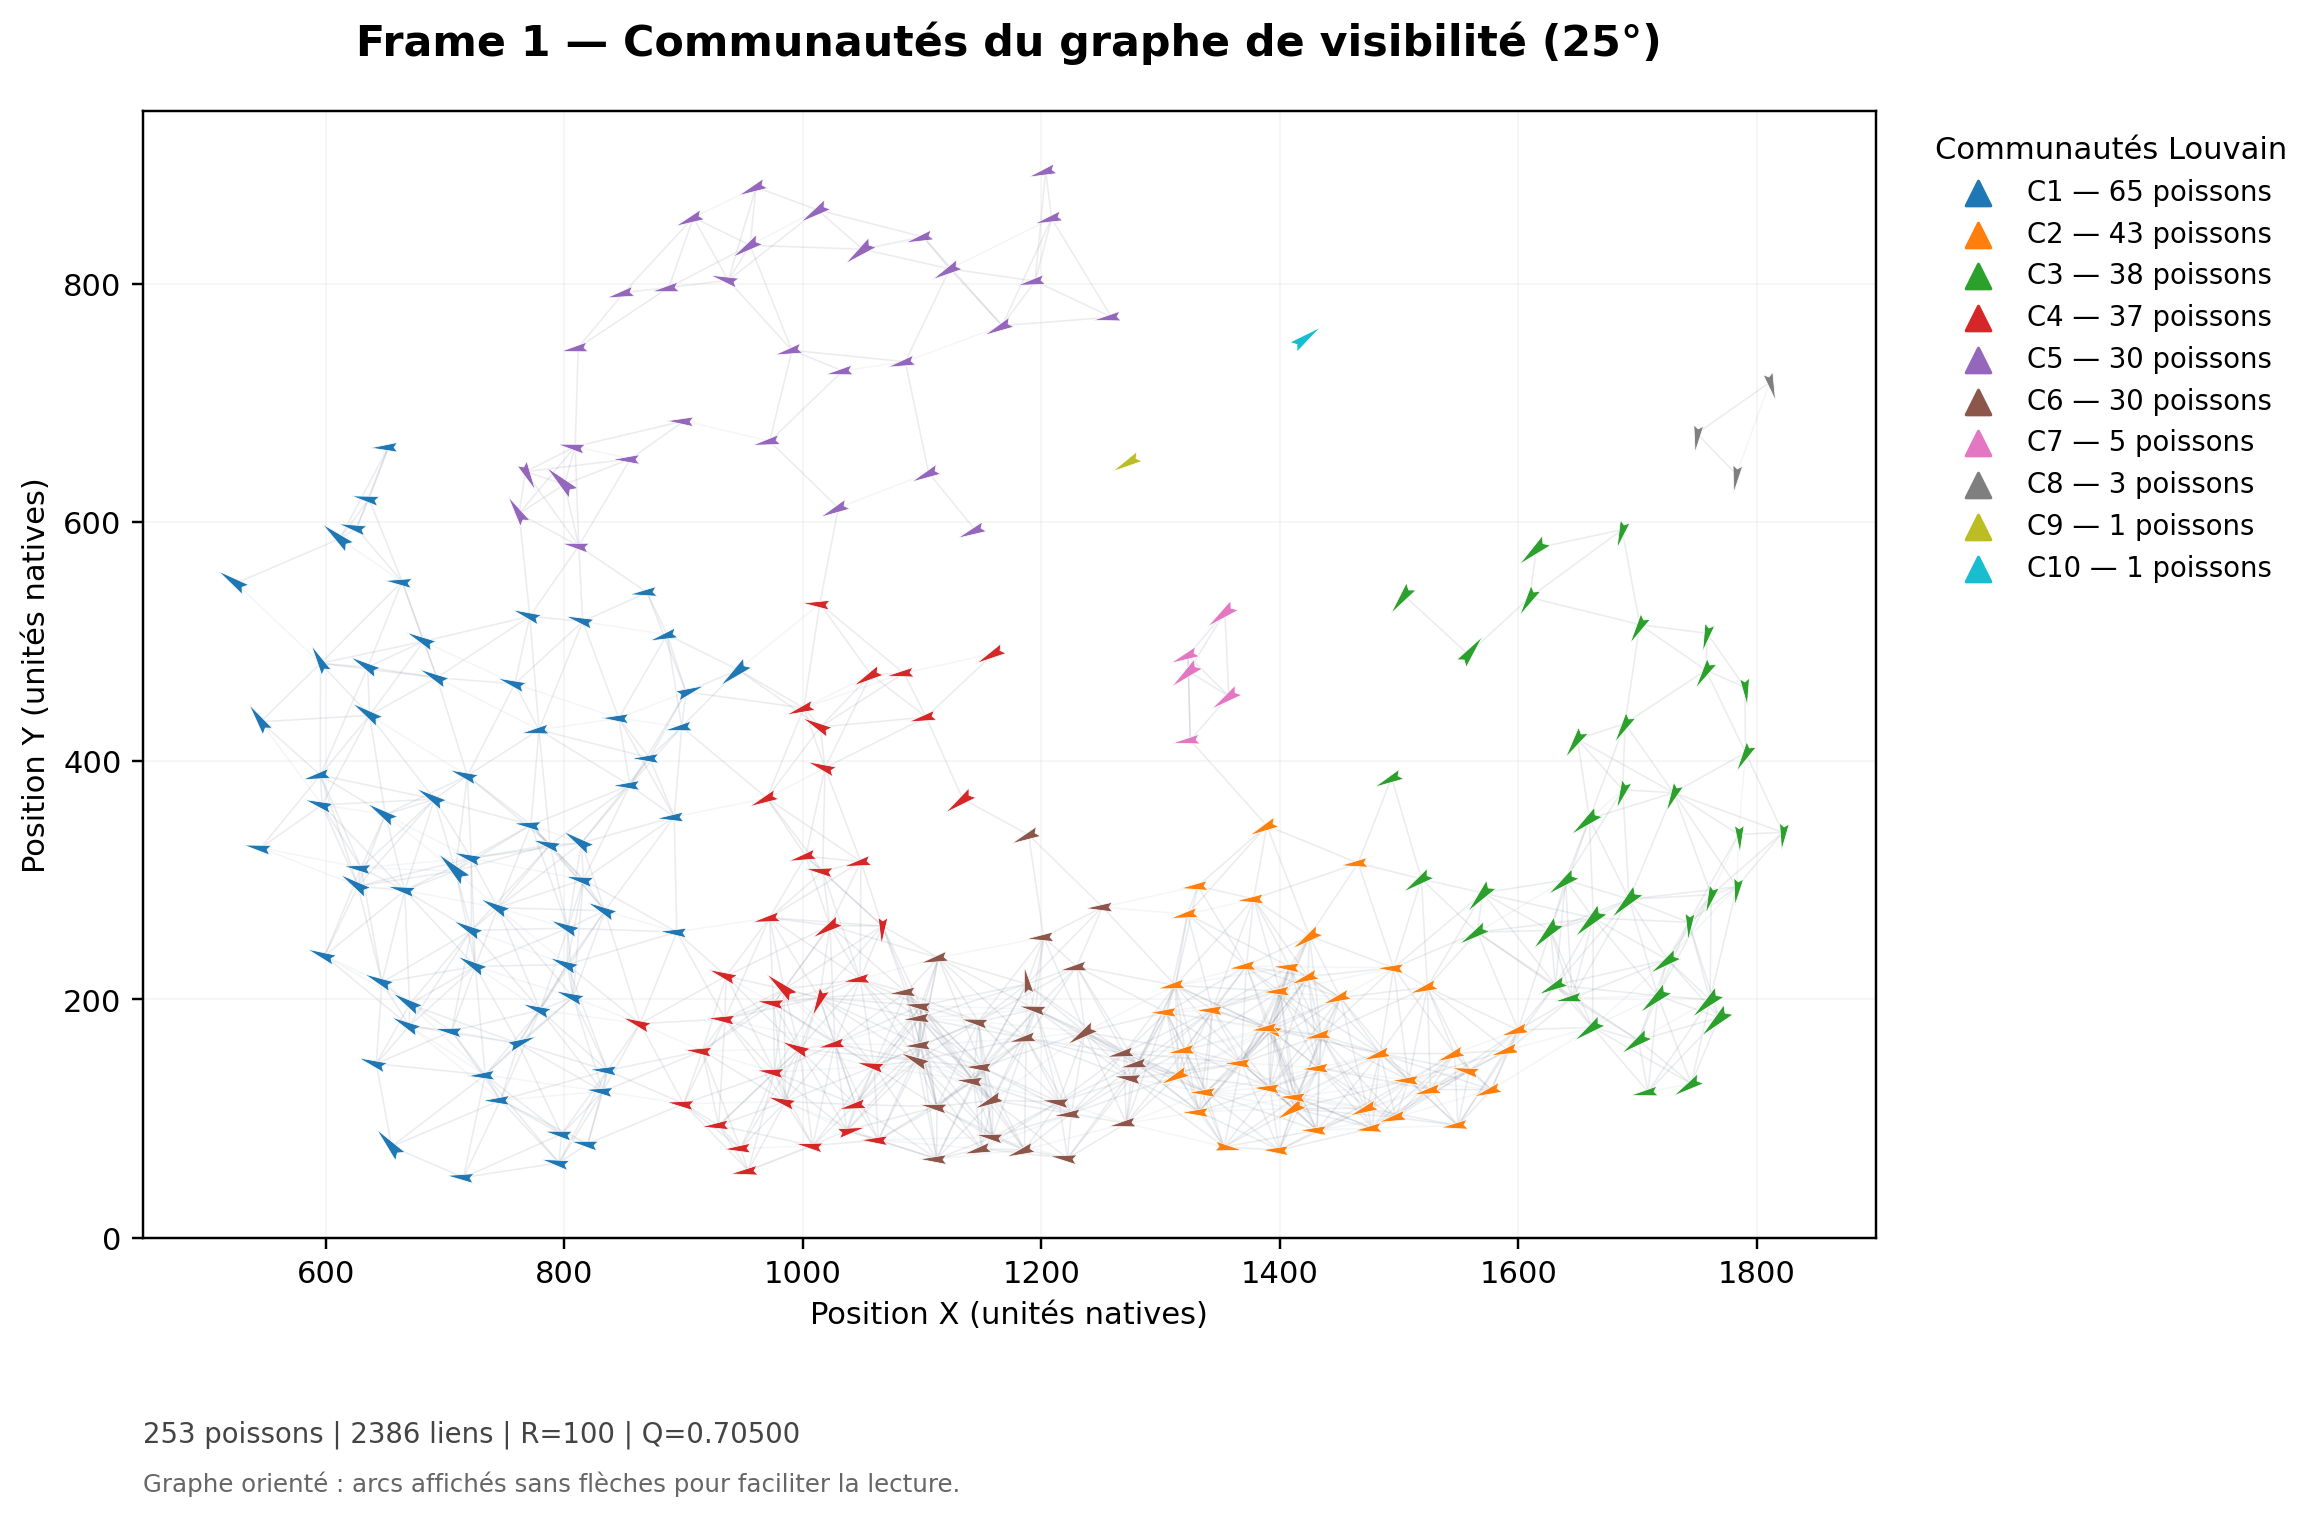
\includegraphics[width=\linewidth]
        {frame1_visibility25_louvain.png}
        \caption{Directed visibility network.}
        \label{fig:visibility_communities}
    \end{subfigure}



    \caption{Louvain community partitions in
    the first experimental frame. Both networks
    contain 253 fish, with a neighbourhood radius
    of $R=100$ and a rear blind angle of
    $25^\circ$ for the visibility model.
    Colours identify independently detected
    communities in each graph. The directed
    arcs of the visibility network are
    represented without arrowheads to
    improve readability.}

    \label{fig:community_comparison}
\end{figure}

The visualisations reveal a pronounced spatial
organisation of the detected communities.
Several groups occupy geographically concentrated
regions of the school, whereas the central
region contains individuals assigned to
different communities.

The introduction of the directional visibility
constraint modifies the distribution of
individuals among the detected groups.
Nevertheless, the modularity values remain
remarkably close, indicating that the overall
strength of the detected community structure
is similar under the two representations.

An important distinction must be established
between connected components and communities.
A graph may contain a single dominant connected
component while still exhibiting several
internally differentiated communities.
These two properties therefore describe
different aspects of network organisation.

However, the interpretation of the detected
communities requires particular caution.
Since connections are constructed from spatial
proximity and directional visibility, the
geometrical configuration of the fish school
may itself generate relatively dense
substructures.

Consequently, the community partitions
should be interpreted as topological
descriptions of the observed network
rather than direct evidence of stable
biological or social subgroups.

\FloatBarrier


\subsection{Temporal Variations in Network Organisation}
\label{subsec:temporal_variations}

The analysis of a single experimental frame provides
a detailed description of the network at a particular
instant. However, fish schooling is a dynamic
phenomenon, and its structural organisation may
evolve throughout the recording.

To investigate these variations, 21 experimental
frames were selected across the observation period.
For each frame, both graph representations were
constructed using the same neighbourhood radius
of $R=100$ and a rear blind angle of $25^\circ$.

The temporal analysis considers the number of
observed individuals, graph density, connectivity,
clustering and community modularity.

\paragraph{Number of observed fish and network density}

The number of observed individuals varies
considerably throughout the sampled sequence.
The smallest observation contains 91 fish,
whereas the largest contains 280 individuals.

Figure~\ref{fig:temporal_population_density}
presents these variations together with
the corresponding evolution of graph density.

\begin{figure}[htbp]
    \centering

    \begin{subfigure}[t]{0.49\textwidth}
        \centering
        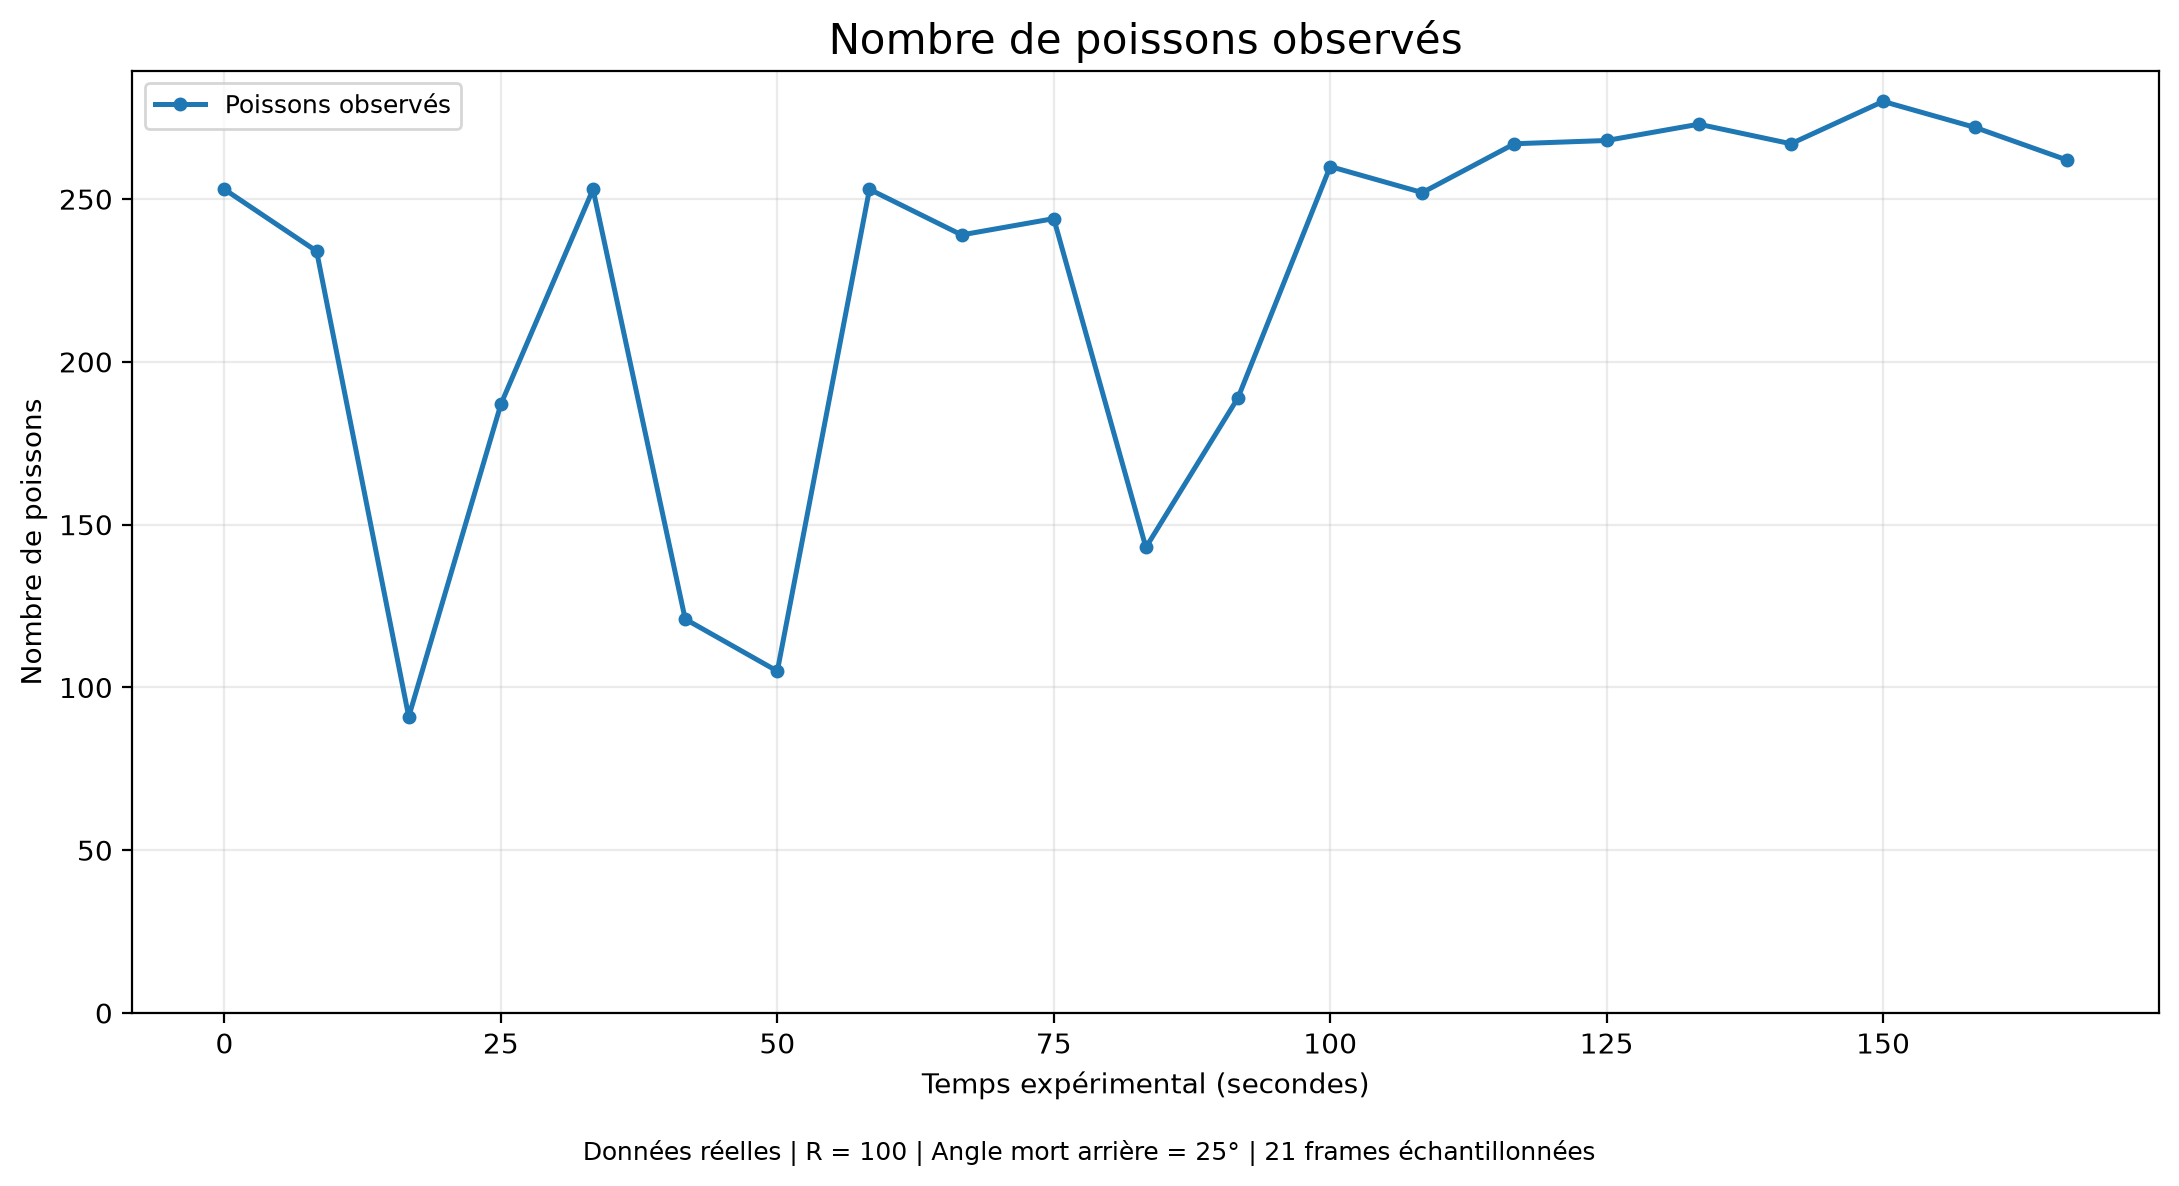
\includegraphics[width=\linewidth]
        {temporal_fish_count.png}
        \caption{Number of observed fish.}
        \label{fig:temporal_fish_count}
    \end{subfigure}
    \hfill
    \begin{subfigure}[t]{0.49\textwidth}
        \centering
        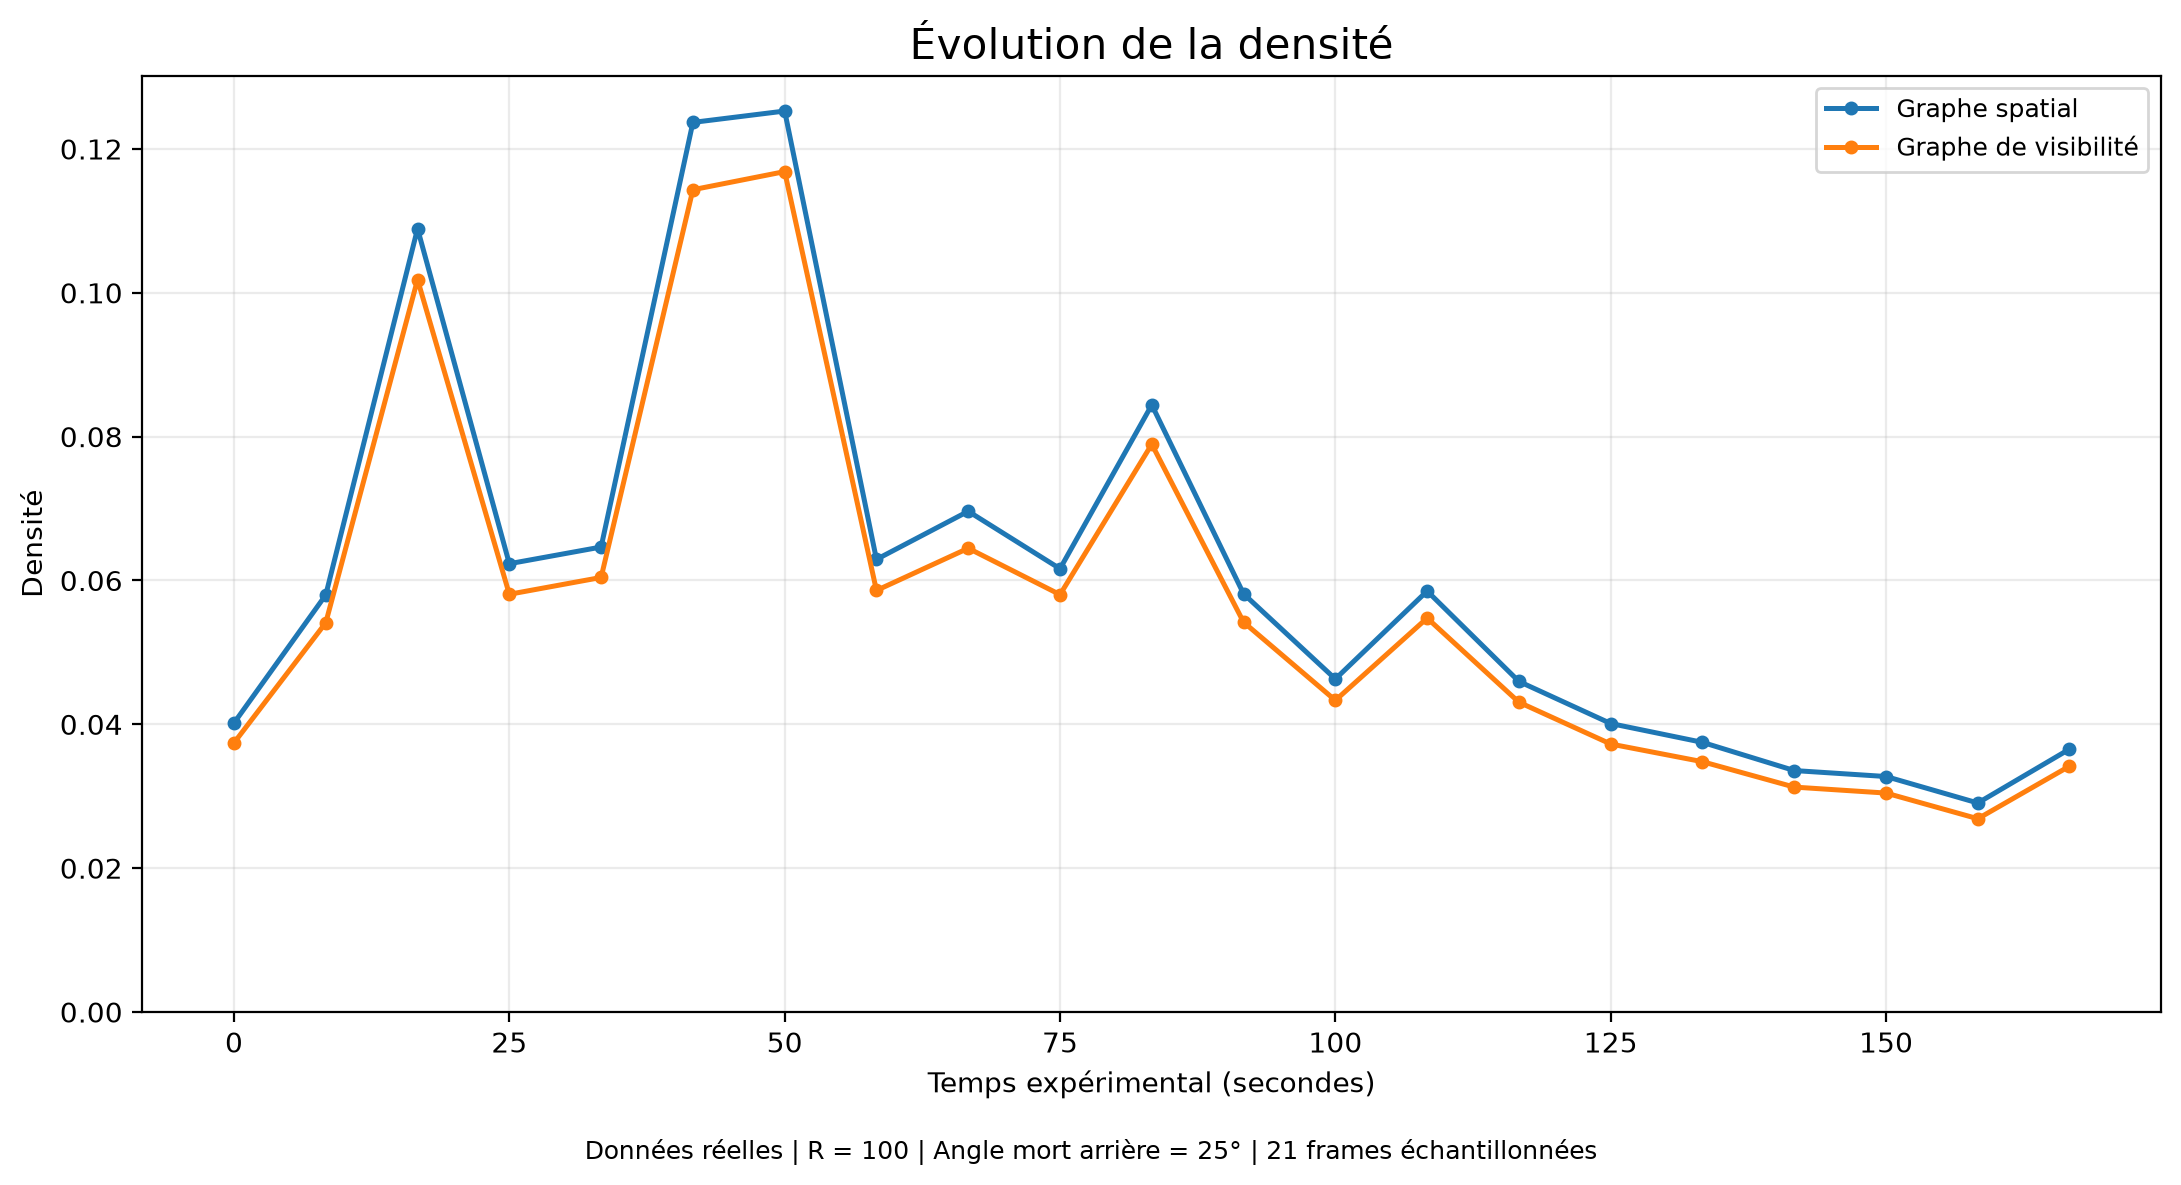
\includegraphics[width=\linewidth]
        {temporal_density.png}
        \caption{Evolution of graph density.}
        \label{fig:temporal_density}
    \end{subfigure}

    \caption{Temporal evolution of the number
    of observed fish and the density of the
    spatial and visibility networks across
    21 sampled frames. The neighbourhood
    radius is $R=100$, with a rear blind
    angle of $25^\circ$ for the visibility
    network.}

    \label{fig:temporal_population_density}
\end{figure}

The first part of the recording exhibits
substantial fluctuations in the number
of detected individuals, followed by
comparatively higher and more stable
observations towards the end.

The spatial graph density ranges from
approximately 0.029 to 0.125.
The visibility graph follows a similar
temporal trajectory, although its
density remains consistently lower.

This difference is consistent with
the additional directional restriction
introduced by the visibility model.

Nevertheless, the temporal variations
in graph density cannot be interpreted
independently of the observed population.
Changes in the number of detected fish
modify the number of possible connections
and may influence the measured topology.

Consequently, changes in network density
cannot be attributed exclusively to
modifications in collective behaviour.

\paragraph{Connectivity of the principal components}

The temporal evolution of connectivity
is examined through the relative size
of the largest connected components.

For the spatial graph, the largest
connected component is considered.
For the directed visibility graph,
the largest strongly connected
component is used.

Figure~\ref{fig:temporal_connectivity}
presents the corresponding results.

\begin{figure}[htbp]
    \centering

    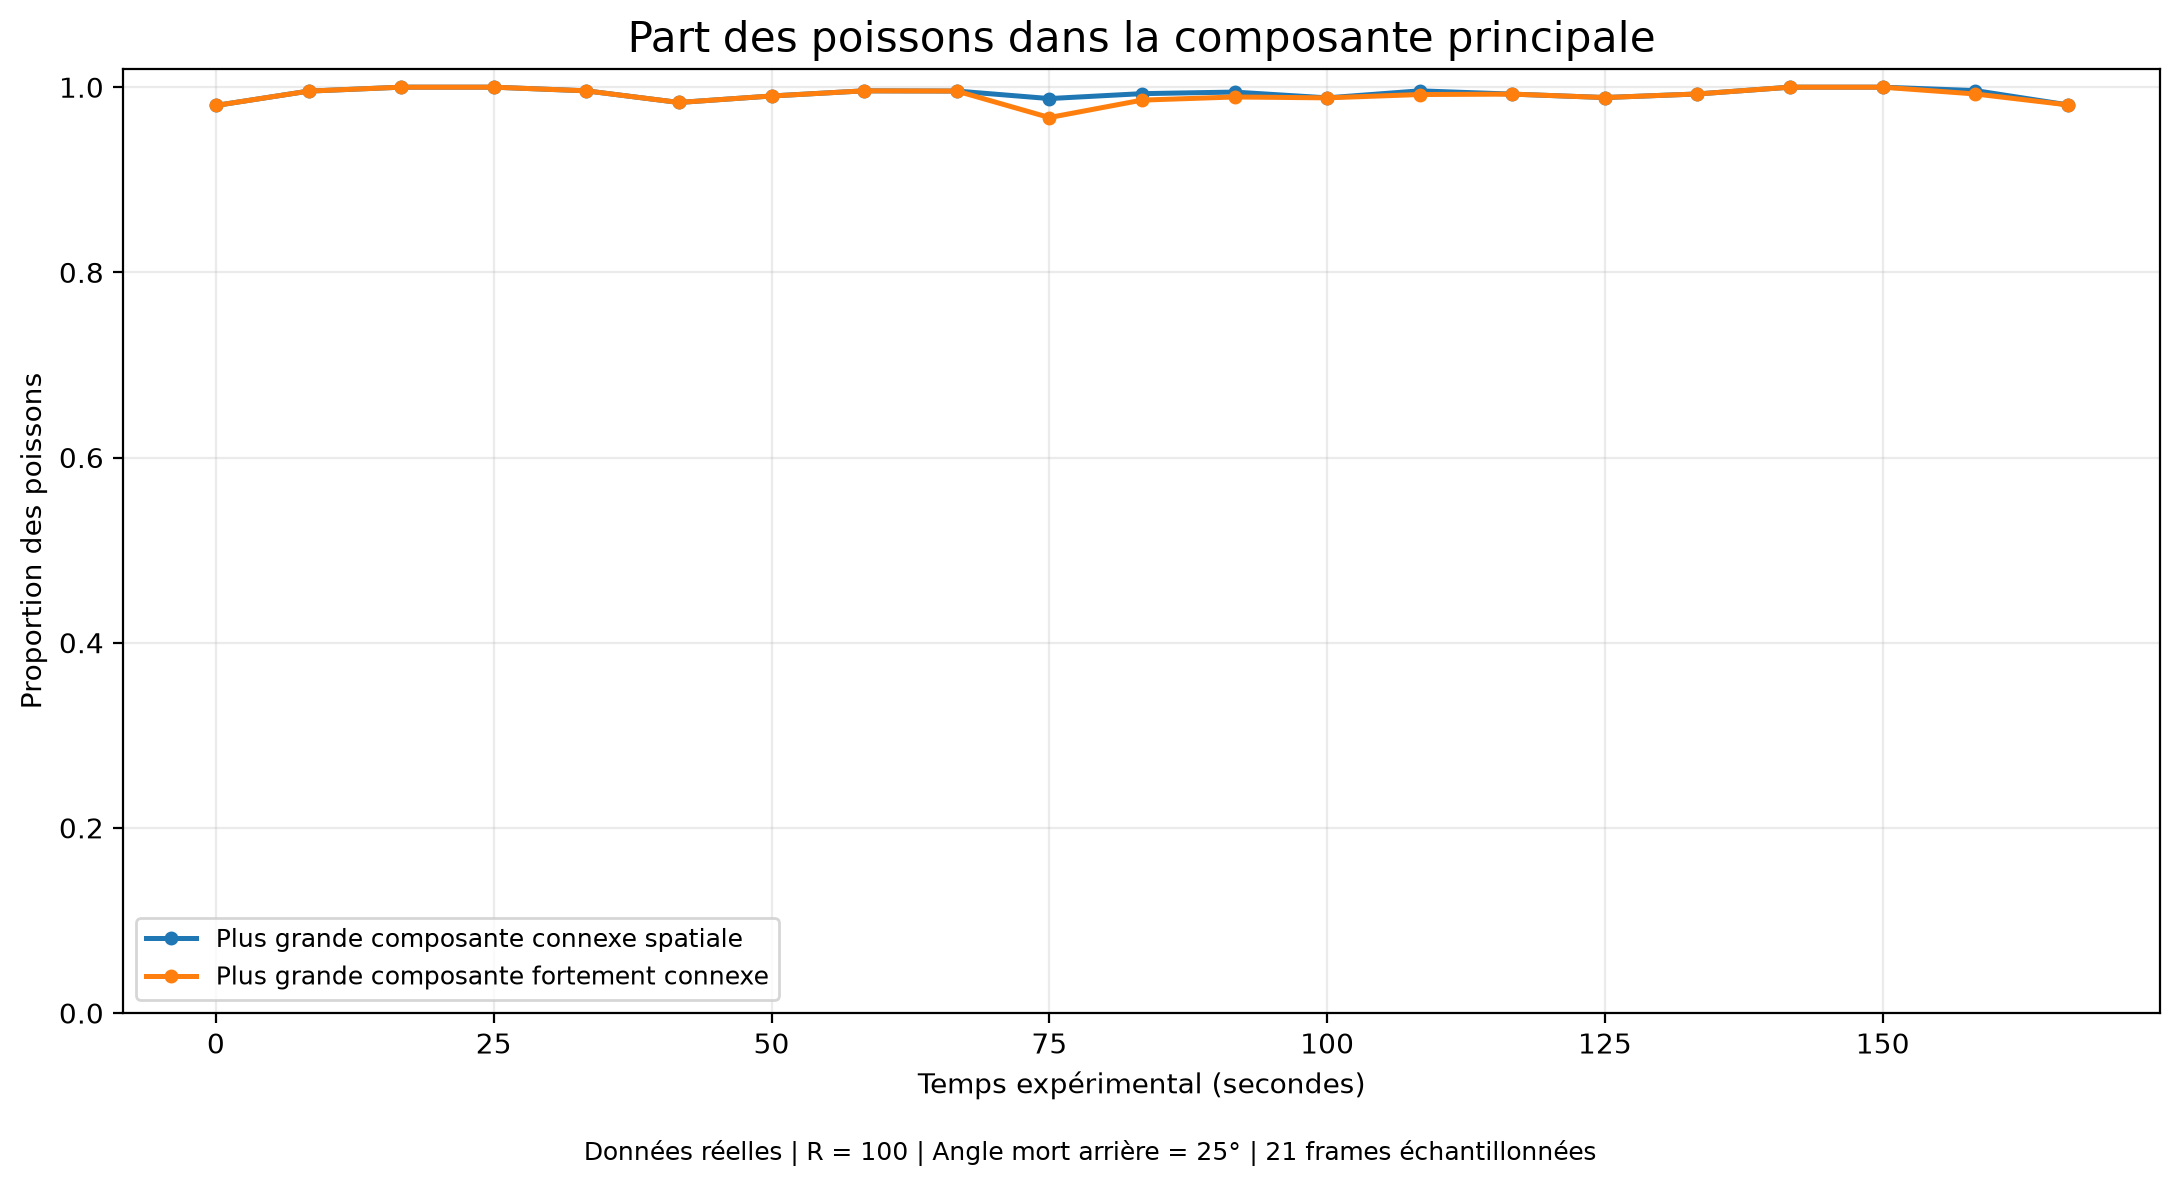
\includegraphics[width=0.82\textwidth]
    {temporal_connectivity.png}

    \caption{Temporal evolution of the
    proportion of observed fish belonging
    to the largest connected component
    of the spatial graph and the largest
    strongly connected component of
    the directed visibility graph.}

    \label{fig:temporal_connectivity}
\end{figure}

The spatial graph exhibits a particularly
high level of global connectivity.
The proportion of fish belonging to
its largest connected component remains
between approximately 98\% and 100\%.

The visibility graph displays a closely
related pattern, with the largest strongly
connected component containing almost
all observed individuals.

These results indicate that the principal
network structure remains largely connected
throughout the sampled sequence, despite
variations in the observed population
and network density.

However, the persistence of a dominant
connected component does not imply that
the same individuals maintain identical
relationships throughout the experiment.

Connectivity describes the existence
of paths within each observed network,
rather than the temporal persistence
of individual connections.

\paragraph{Clustering and community modularity}

The evolution of local clustering and
community modularity provides additional
information about the internal organisation
of the fish school.

Figure~\ref{fig:temporal_clustering_modularity}
compares these measures for the spatial
and visibility networks.

\begin{figure}[htbp]
    \centering

    \begin{subfigure}[t]{0.49\textwidth}
        \centering
        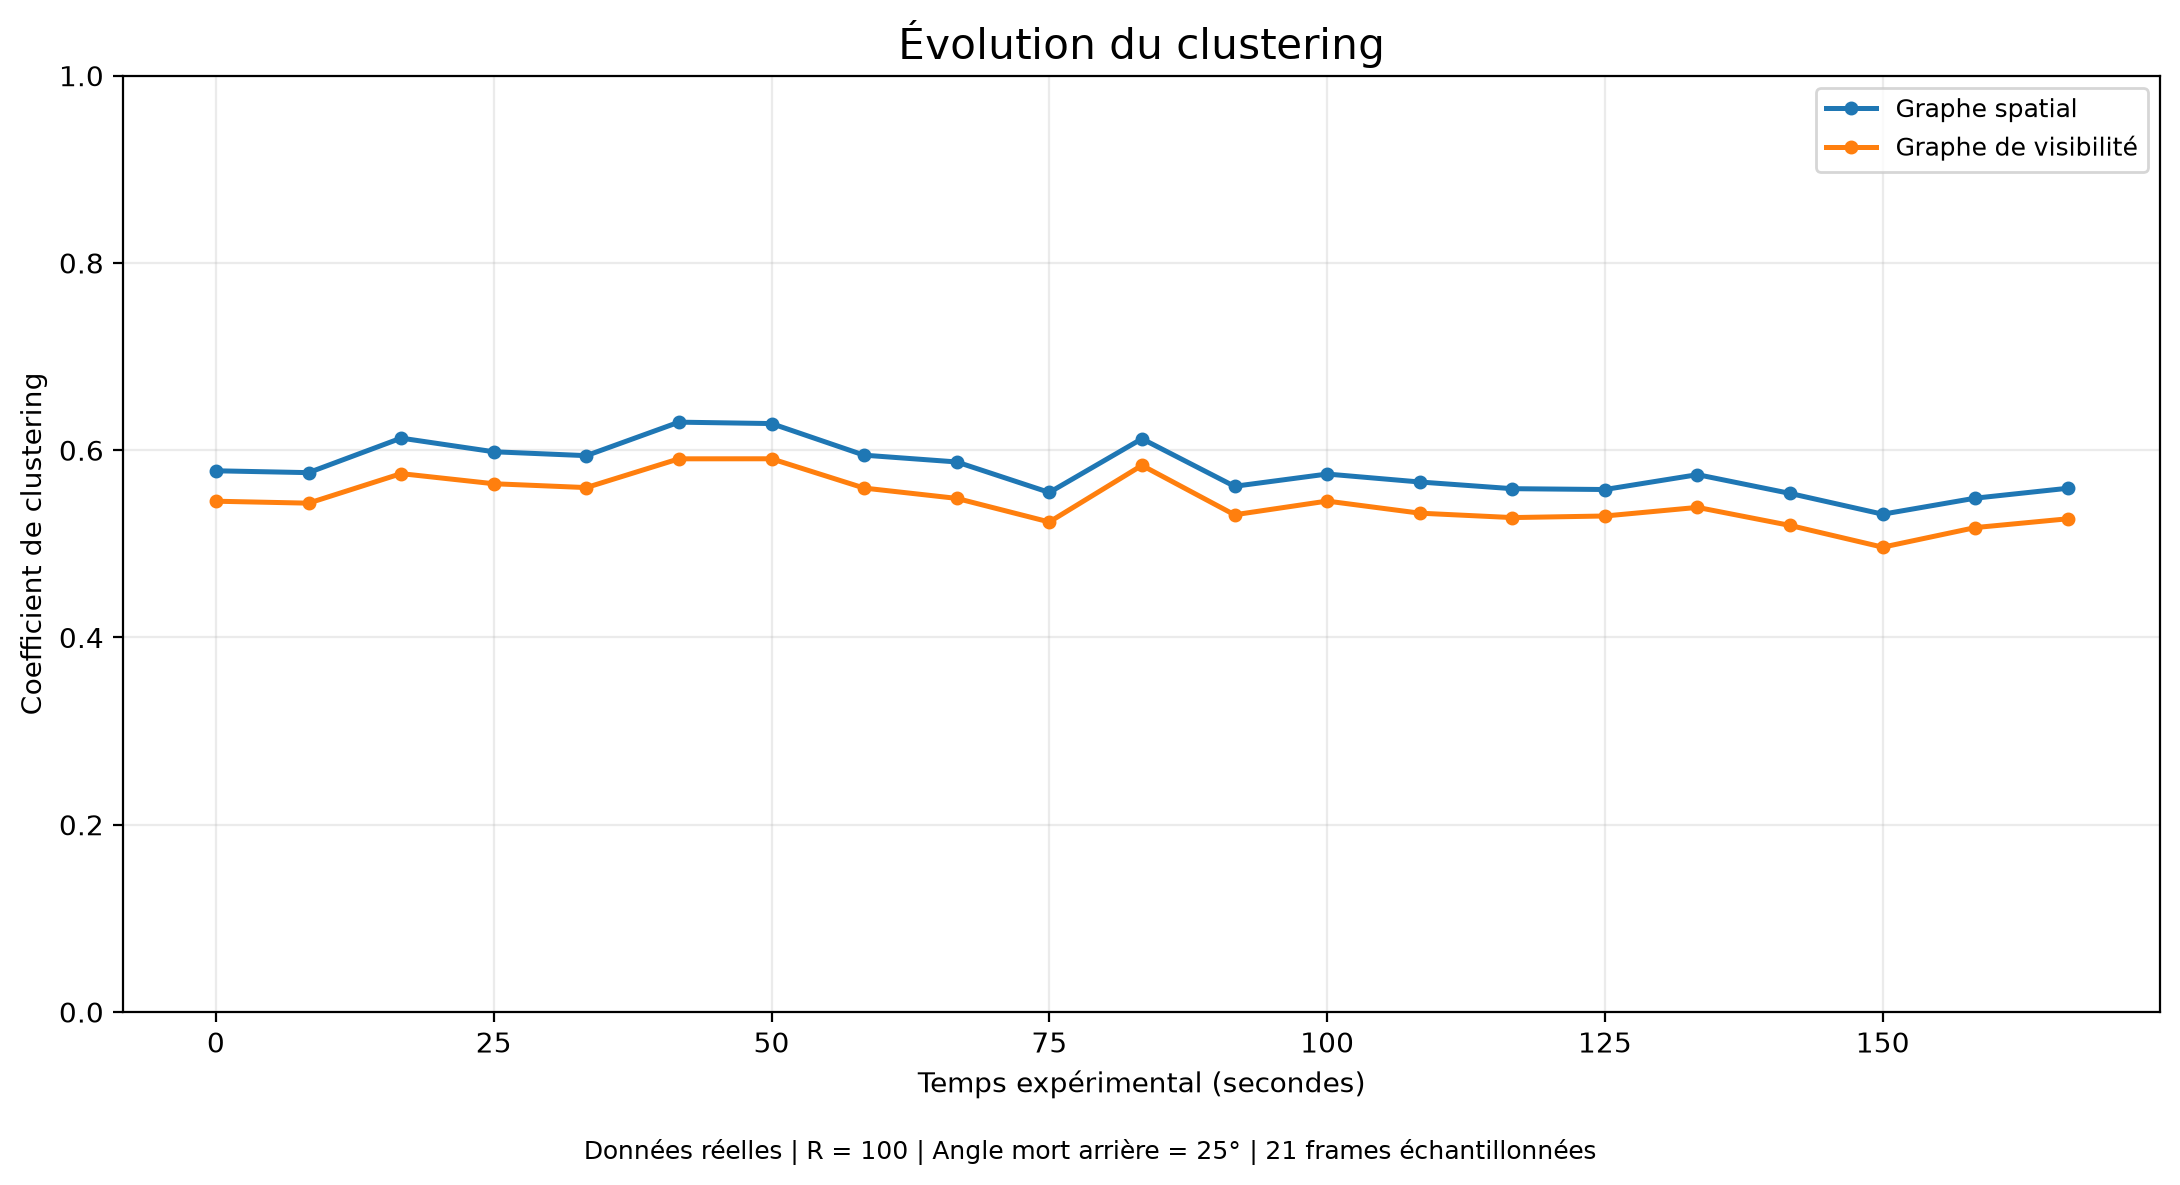
\includegraphics[width=\linewidth]
        {temporal_clustering.png}
        \caption{Average clustering coefficient.}
        \label{fig:temporal_clustering}
    \end{subfigure}
    \hfill
    \begin{subfigure}[t]{0.49\textwidth}
        \centering
        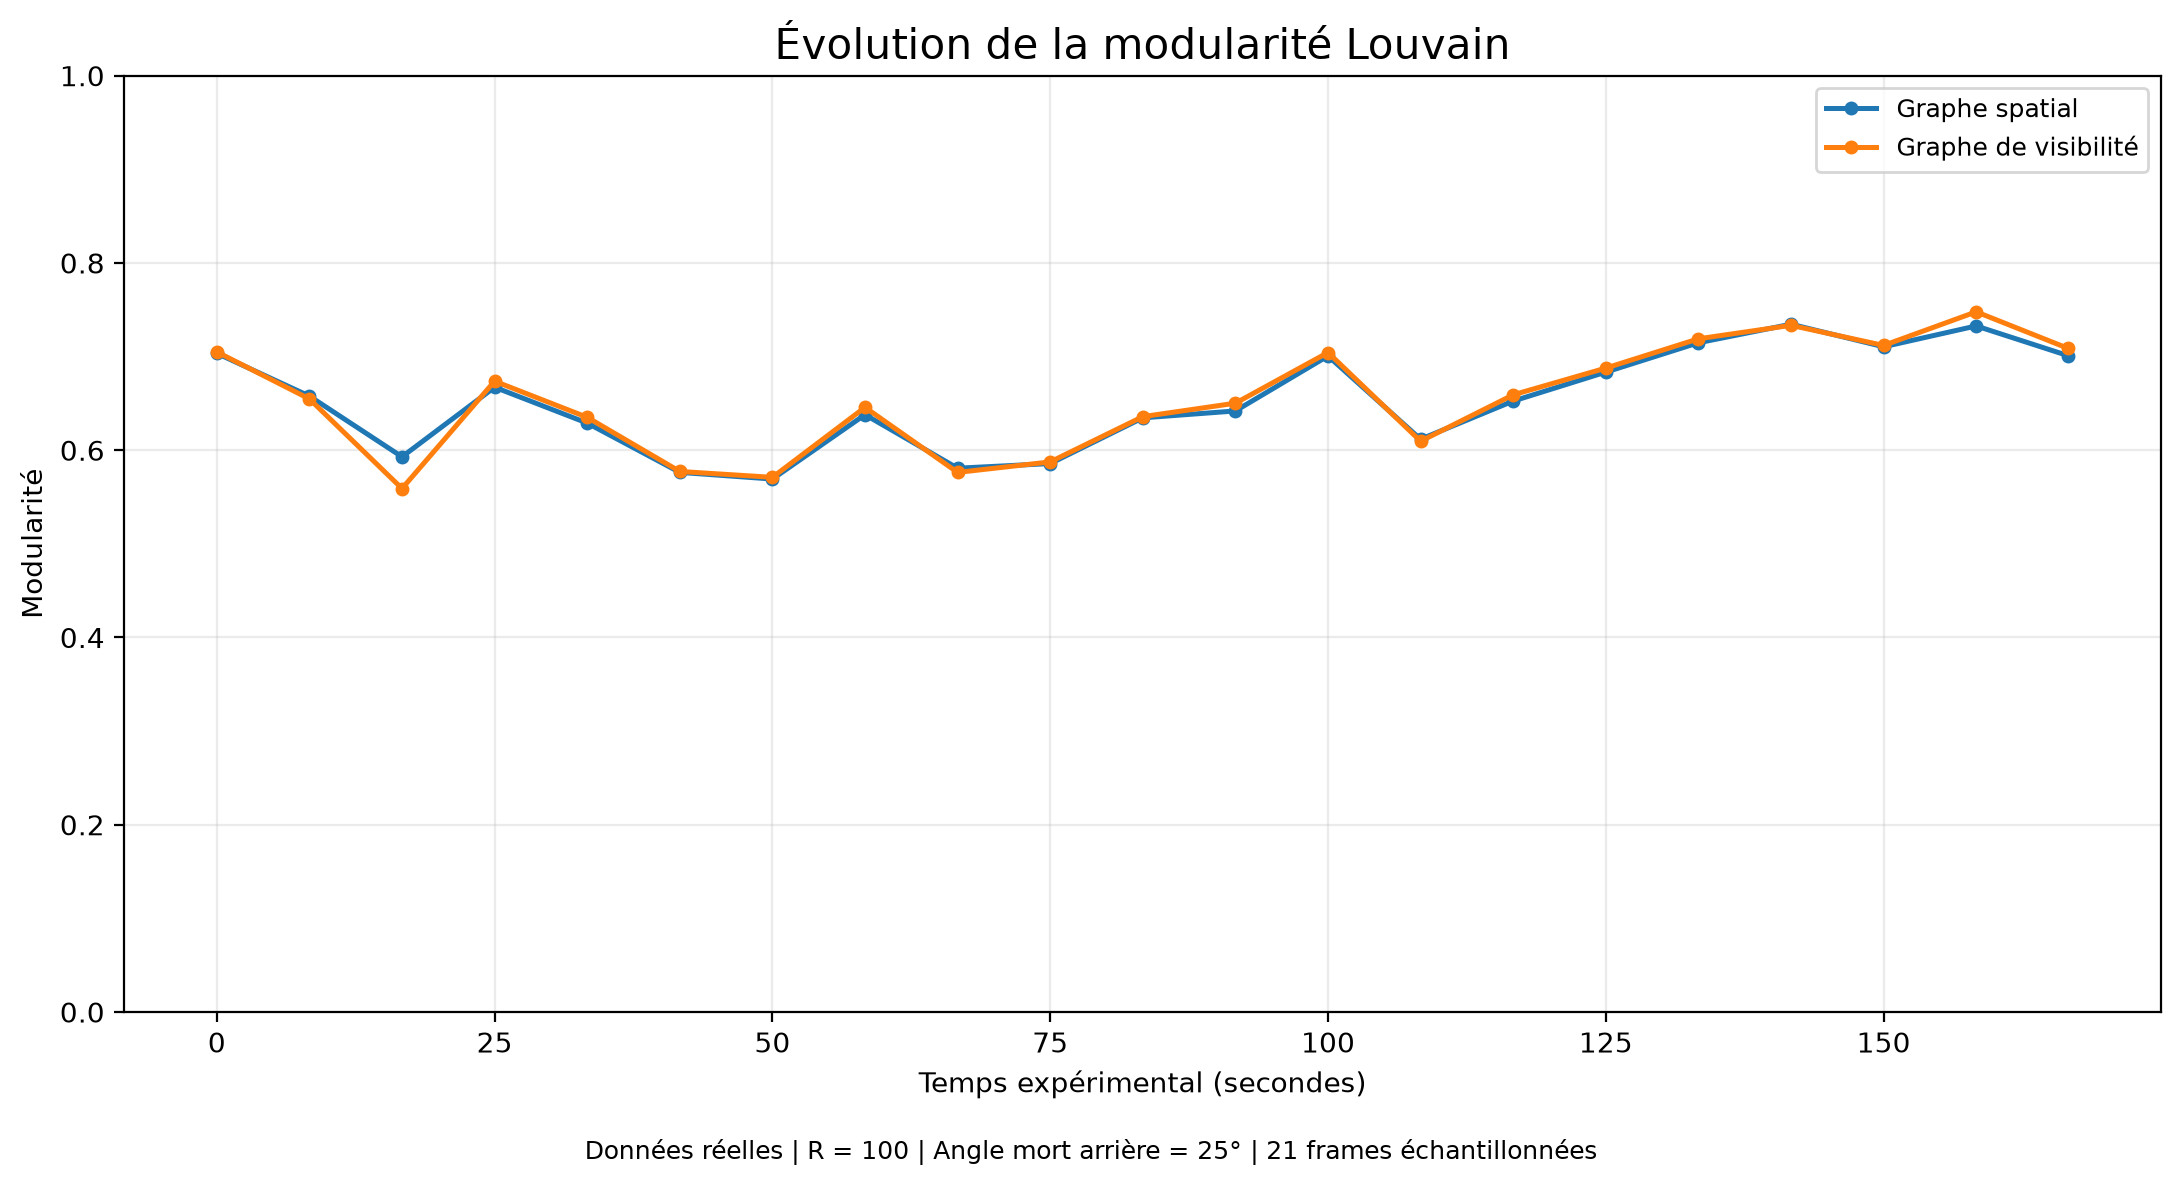
\includegraphics[width=\linewidth]
        {temporal_modularity.png}
        \caption{Louvain modularity.}
        \label{fig:temporal_modularity}
    \end{subfigure}

    \caption{Temporal evolution of the
    average clustering coefficient and
    Louvain modularity for both network
    representations, evaluated across
    the same 21 sampled frames.}

    \label{fig:temporal_clustering_modularity}
\end{figure}

The average clustering coefficient remains
relatively high throughout the experimental
sequence. For the spatial graph, it varies
between approximately 0.53 and 0.63.

The visibility graph generally exhibits
slightly lower values while preserving
a similar temporal evolution.

These results indicate that neighbouring
individuals frequently form locally
interconnected groups.

The Louvain modularity also varies
throughout the observation period.
For the spatial graph, values range
from approximately 0.57 to 0.73.

The two models follow closely related
modularity trajectories, suggesting
that the additional directional
constraint does not substantially
modify the overall temporal pattern
of community organisation under
the selected parameters.

Nevertheless, variations in modularity
may result from changes in spatial
configuration, the number of detected
individuals or the community partitions
identified by the algorithm.

The temporal analysis therefore reveals
a network structure characterised by
high global connectivity, relatively
pronounced local clustering and
persistent modular organisation
at the level of the sampled graphs.

These observations provide evidence
of structural regularities in the
constructed networks, but do not
establish the existence of fixed
social relationships or causal
interaction mechanisms.

\FloatBarrier


\subsection{Sensitivity to the Neighbourhood Radius}
\label{subsec:radius_sensitivity}

The construction of a spatial proximity graph
requires the selection of a neighbourhood
radius. This parameter determines which
individuals are considered sufficiently
close to establish a connection.

Since the resulting topology depends
directly on this modelling choice,
a sensitivity analysis was conducted
to evaluate its influence on the
main structural measures.

Five neighbourhood radii were considered:

\begin{equation}
R \in \{60,80,100,120,140\}.
\end{equation}

The analysis was performed using the same
21 experimental frames for each radius.
The rear blind angle of the visibility
graph was maintained at $25^\circ$.

Table~\ref{tab:sensitivity_results}
summarises the mean structural properties
obtained for the spatial graph.

\begin{table}[htbp]
    \centering

    \caption{Mean structural properties
    of the spatial graph across
    21 experimental frames for
    different neighbourhood radii.}

    \label{tab:sensitivity_results}

    \small
    \begin{tabular}{ccccc}
        \hline
        $R$ & Density & Clustering
        & Communities & LCC (\%)\\
        \hline
        60  & 0.02128 & 0.41344 & 29.76 & 78.78\\
        80  & 0.03906 & 0.52683 & 12.90 & 95.14\\
        100 & 0.06095 & 0.57873 & 8.76  & 99.28\\
        120 & 0.08619 & 0.61020 & 6.81  & 99.63\\
        140 & 0.11418 & 0.63357 & 6.43  & 99.71\\
        \hline
    \end{tabular}
\end{table}

\paragraph{Network density and connectivity}

Figure~\ref{fig:sensitivity_density_connectivity}
presents the evolution of network density
and the relative size of the principal
connected components as the neighbourhood
radius increases.

\begin{figure}[htbp]
    \centering

    \begin{subfigure}[t]{0.49\textwidth}
        \centering
        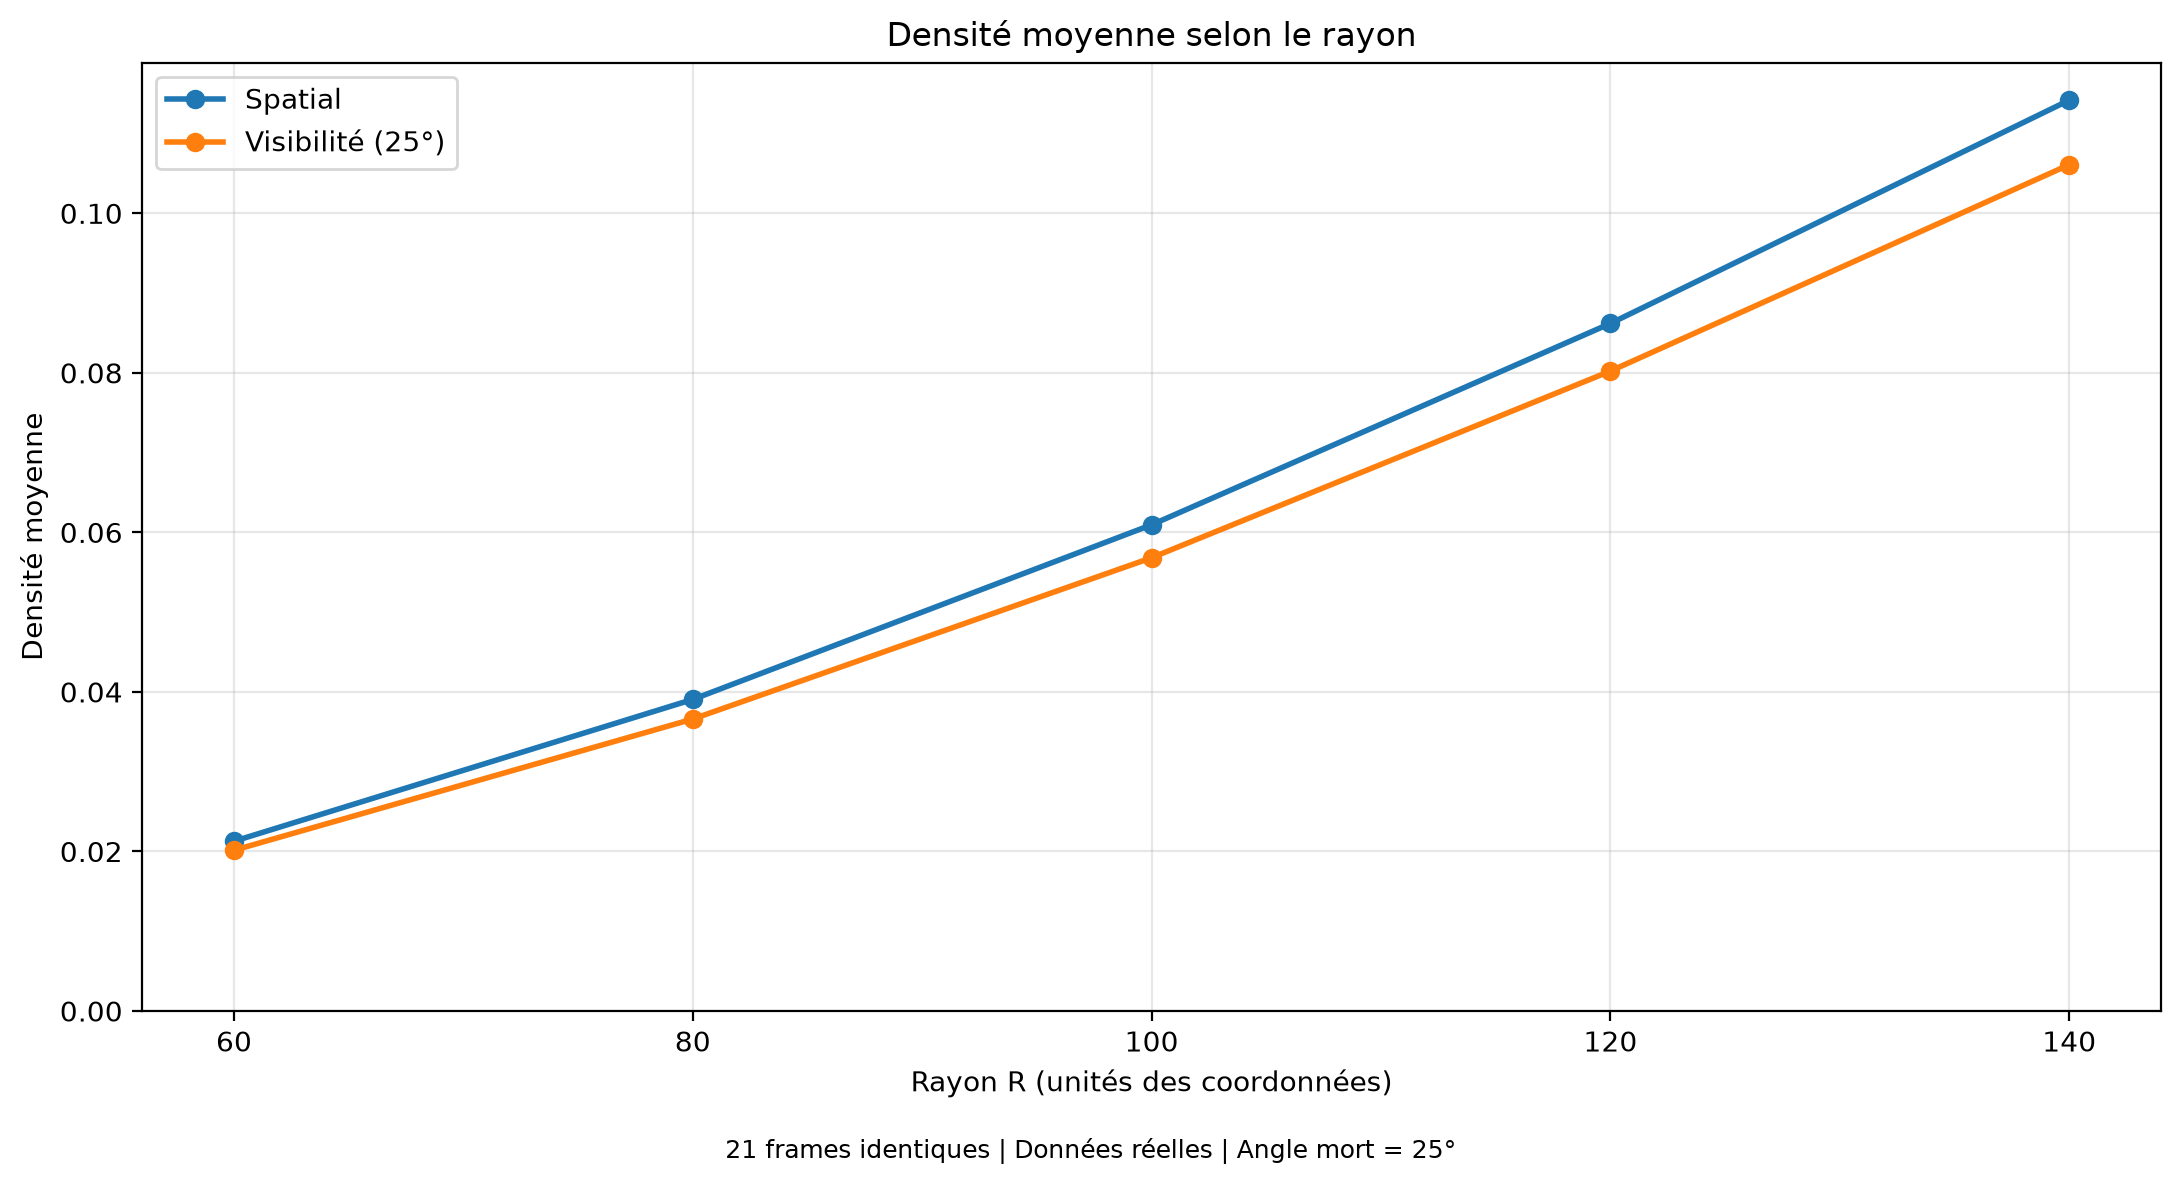
\includegraphics[width=\linewidth]
        {sensitivity_density.png}
        \caption{Mean network density.}
        \label{fig:sensitivity_density}
    \end{subfigure}
    \hfill
    \begin{subfigure}[t]{0.49\textwidth}
        \centering
        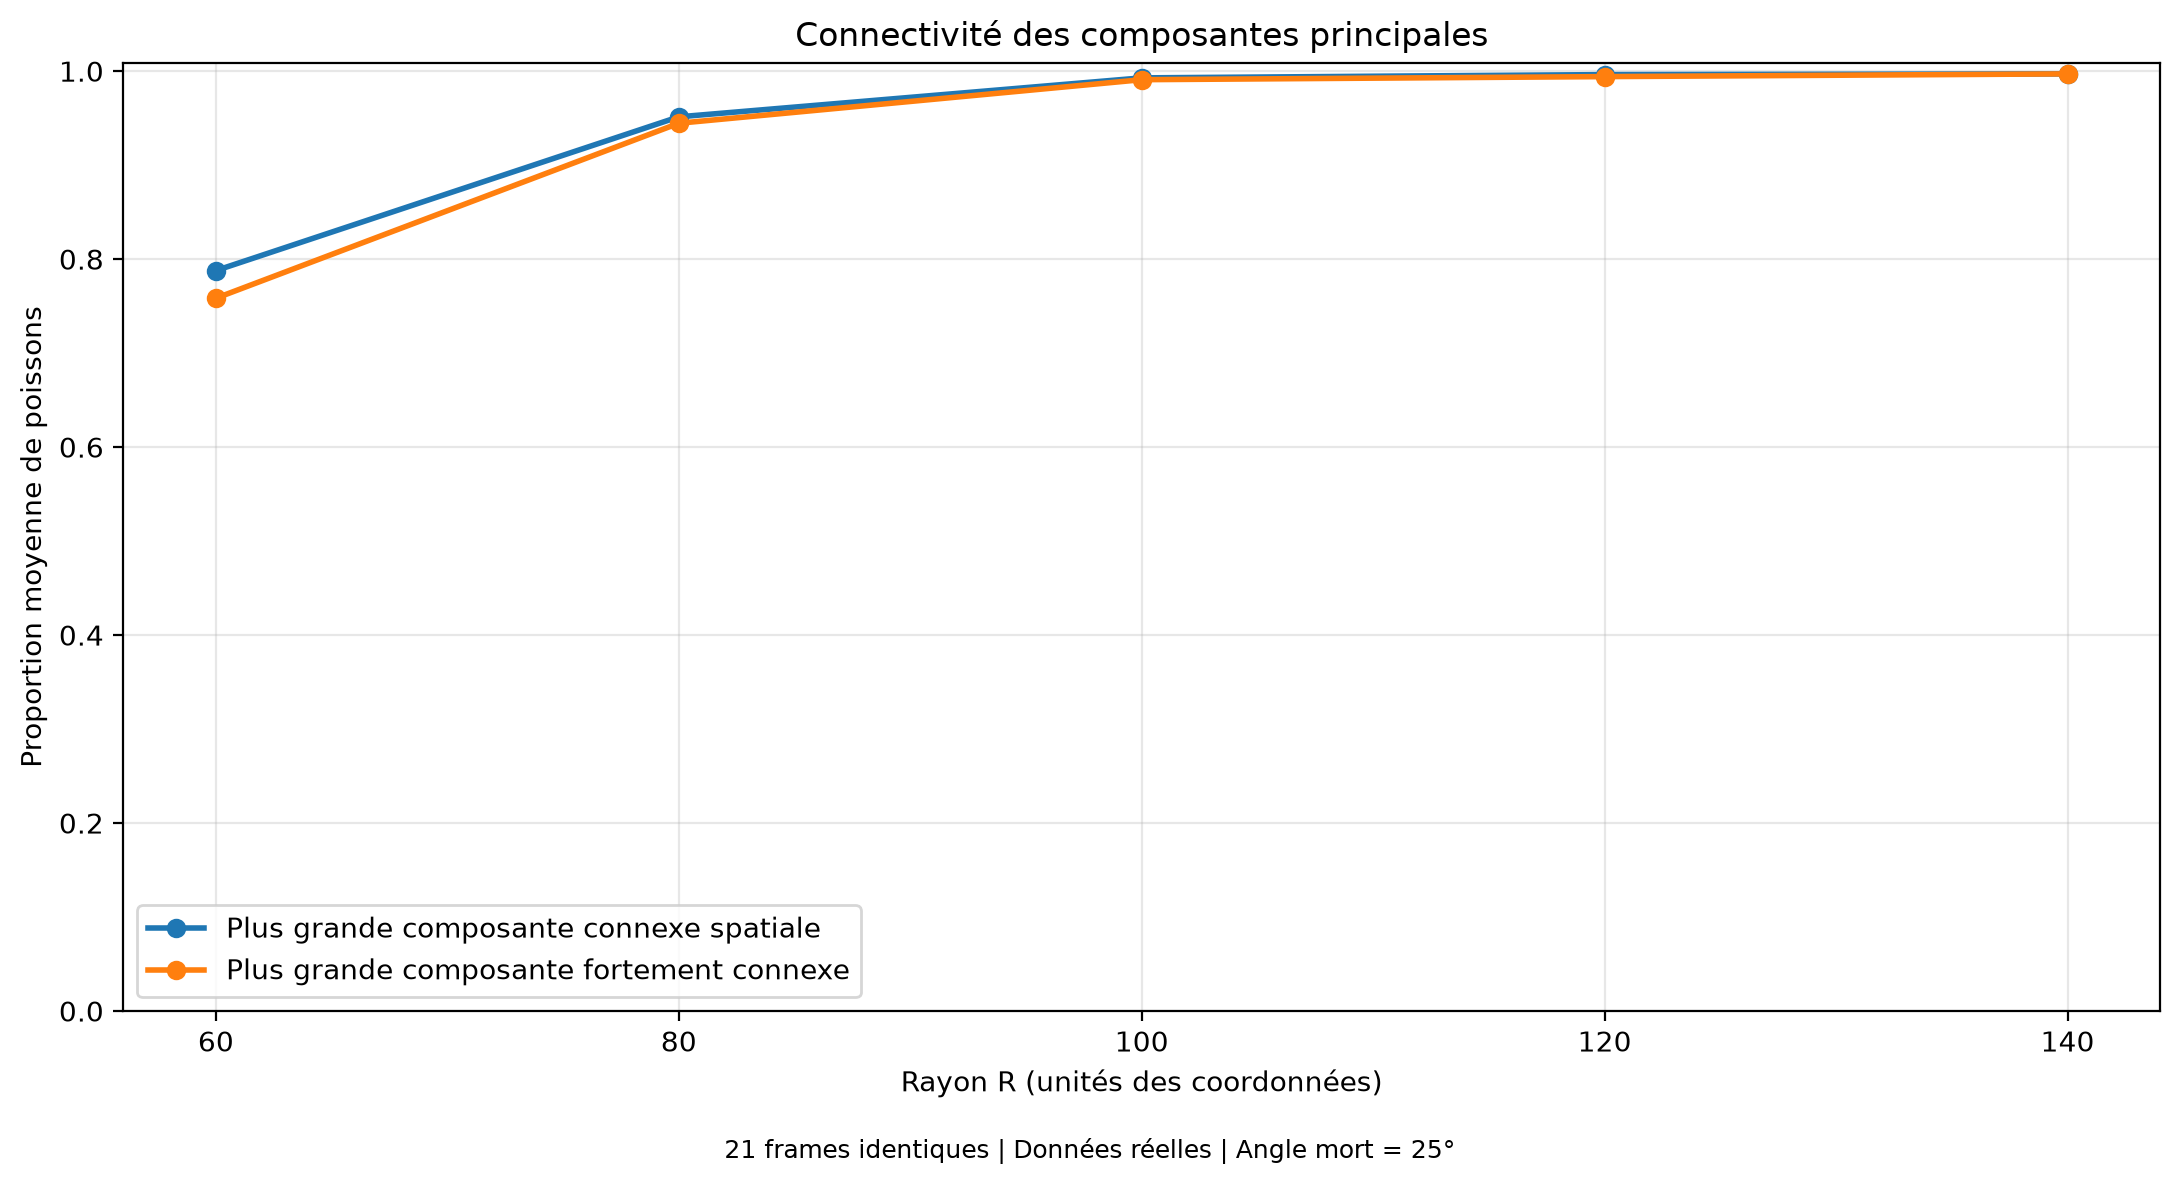
\includegraphics[width=\linewidth]
        {sensitivity_connectivity.png}
        \caption{Largest component share.}
        \label{fig:sensitivity_connectivity}
    \end{subfigure}

    \caption{Influence of the neighbourhood
    radius on network density and the
    relative size of the largest connected
    components. The same 21 frames are
    used for both graph representations.}

    \label{fig:sensitivity_density_connectivity}
\end{figure}

The mean density increases systematically
with the neighbourhood radius.

For the spatial graph, it rises from
0.02128 at $R=60$ to 0.11418 at $R=140$.

The visibility graph exhibits a similar
evolution, although its density remains
slightly lower for every selected radius.

This behaviour follows directly from
the graph construction procedure.
Increasing the neighbourhood radius
introduces additional potential
connections between individuals
whose positions remain unchanged.

The relative size of the largest
connected component also increases
with the neighbourhood radius.

At $R=60$, the largest connected
component of the spatial graph
contains approximately 78.78\%
of the observed individuals.

This proportion increases to 95.14\%
at $R=80$ and 99.28\% at $R=100$.

Beyond $R=100$, the largest component
already contains almost all observed
fish, and further increases in radius
produce relatively limited changes
in global connectivity.

The visibility graph exhibits a
comparable tendency, although its
connectivity is evaluated through
the largest strongly connected component.

These results indicate that the
neighbourhood radius has a particularly
pronounced influence on network
fragmentation at smaller values.

\paragraph{Clustering and community organisation}

The effect of the neighbourhood radius
on local clustering and the number of
detected communities is presented
in Figure~\ref{fig:sensitivity_clustering_communities}.

\begin{figure}[htbp]
    \centering

    \begin{subfigure}[t]{0.49\textwidth}
        \centering
        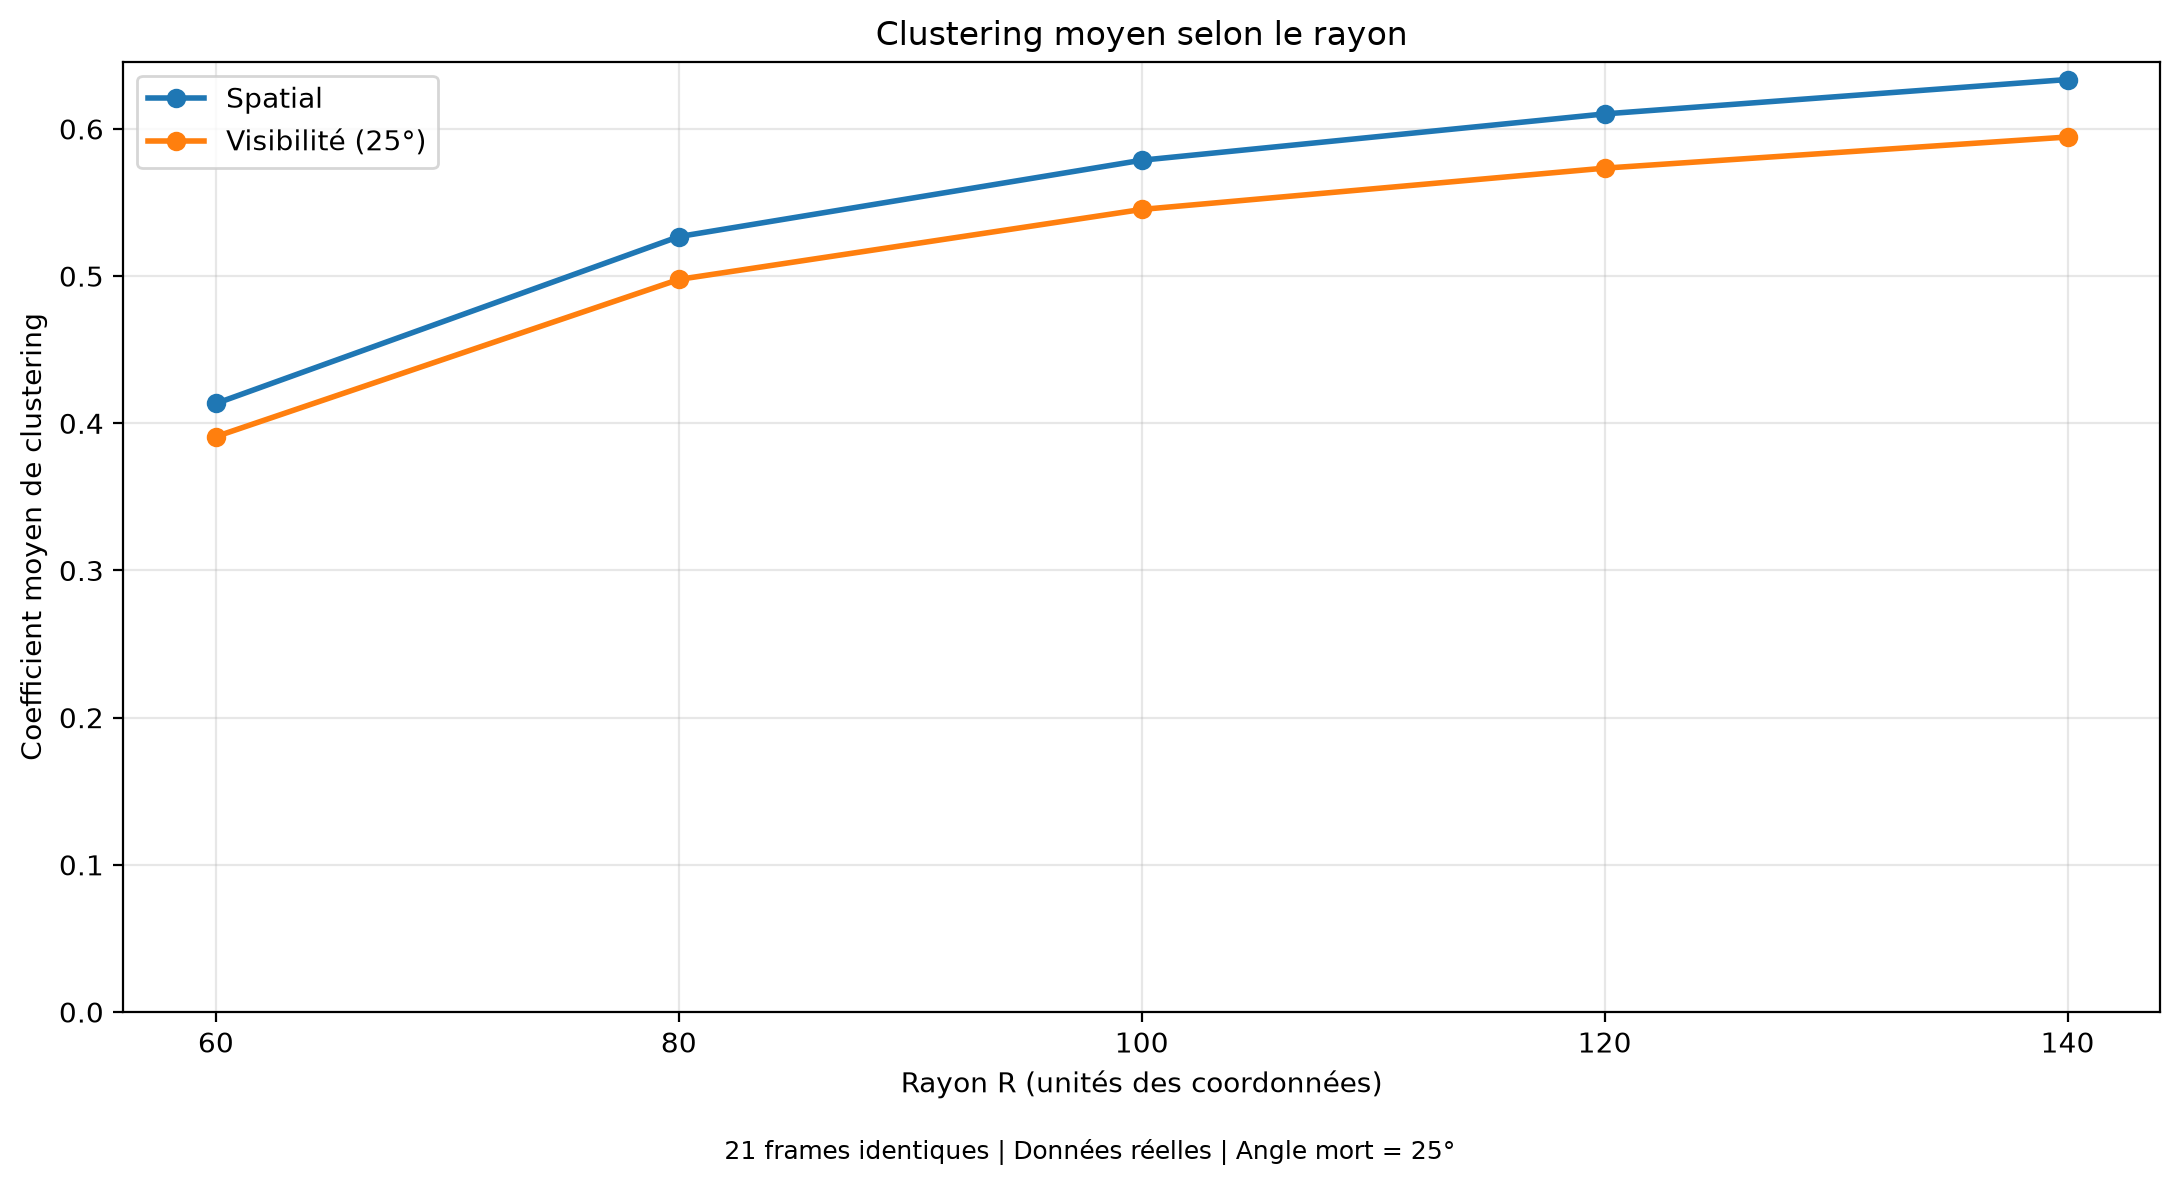
\includegraphics[width=\linewidth]
        {sensitivity_clustering.png}
        \caption{Mean clustering coefficient.}
        \label{fig:sensitivity_clustering}
    \end{subfigure}
    \hfill
    \begin{subfigure}[t]{0.49\textwidth}
        \centering
        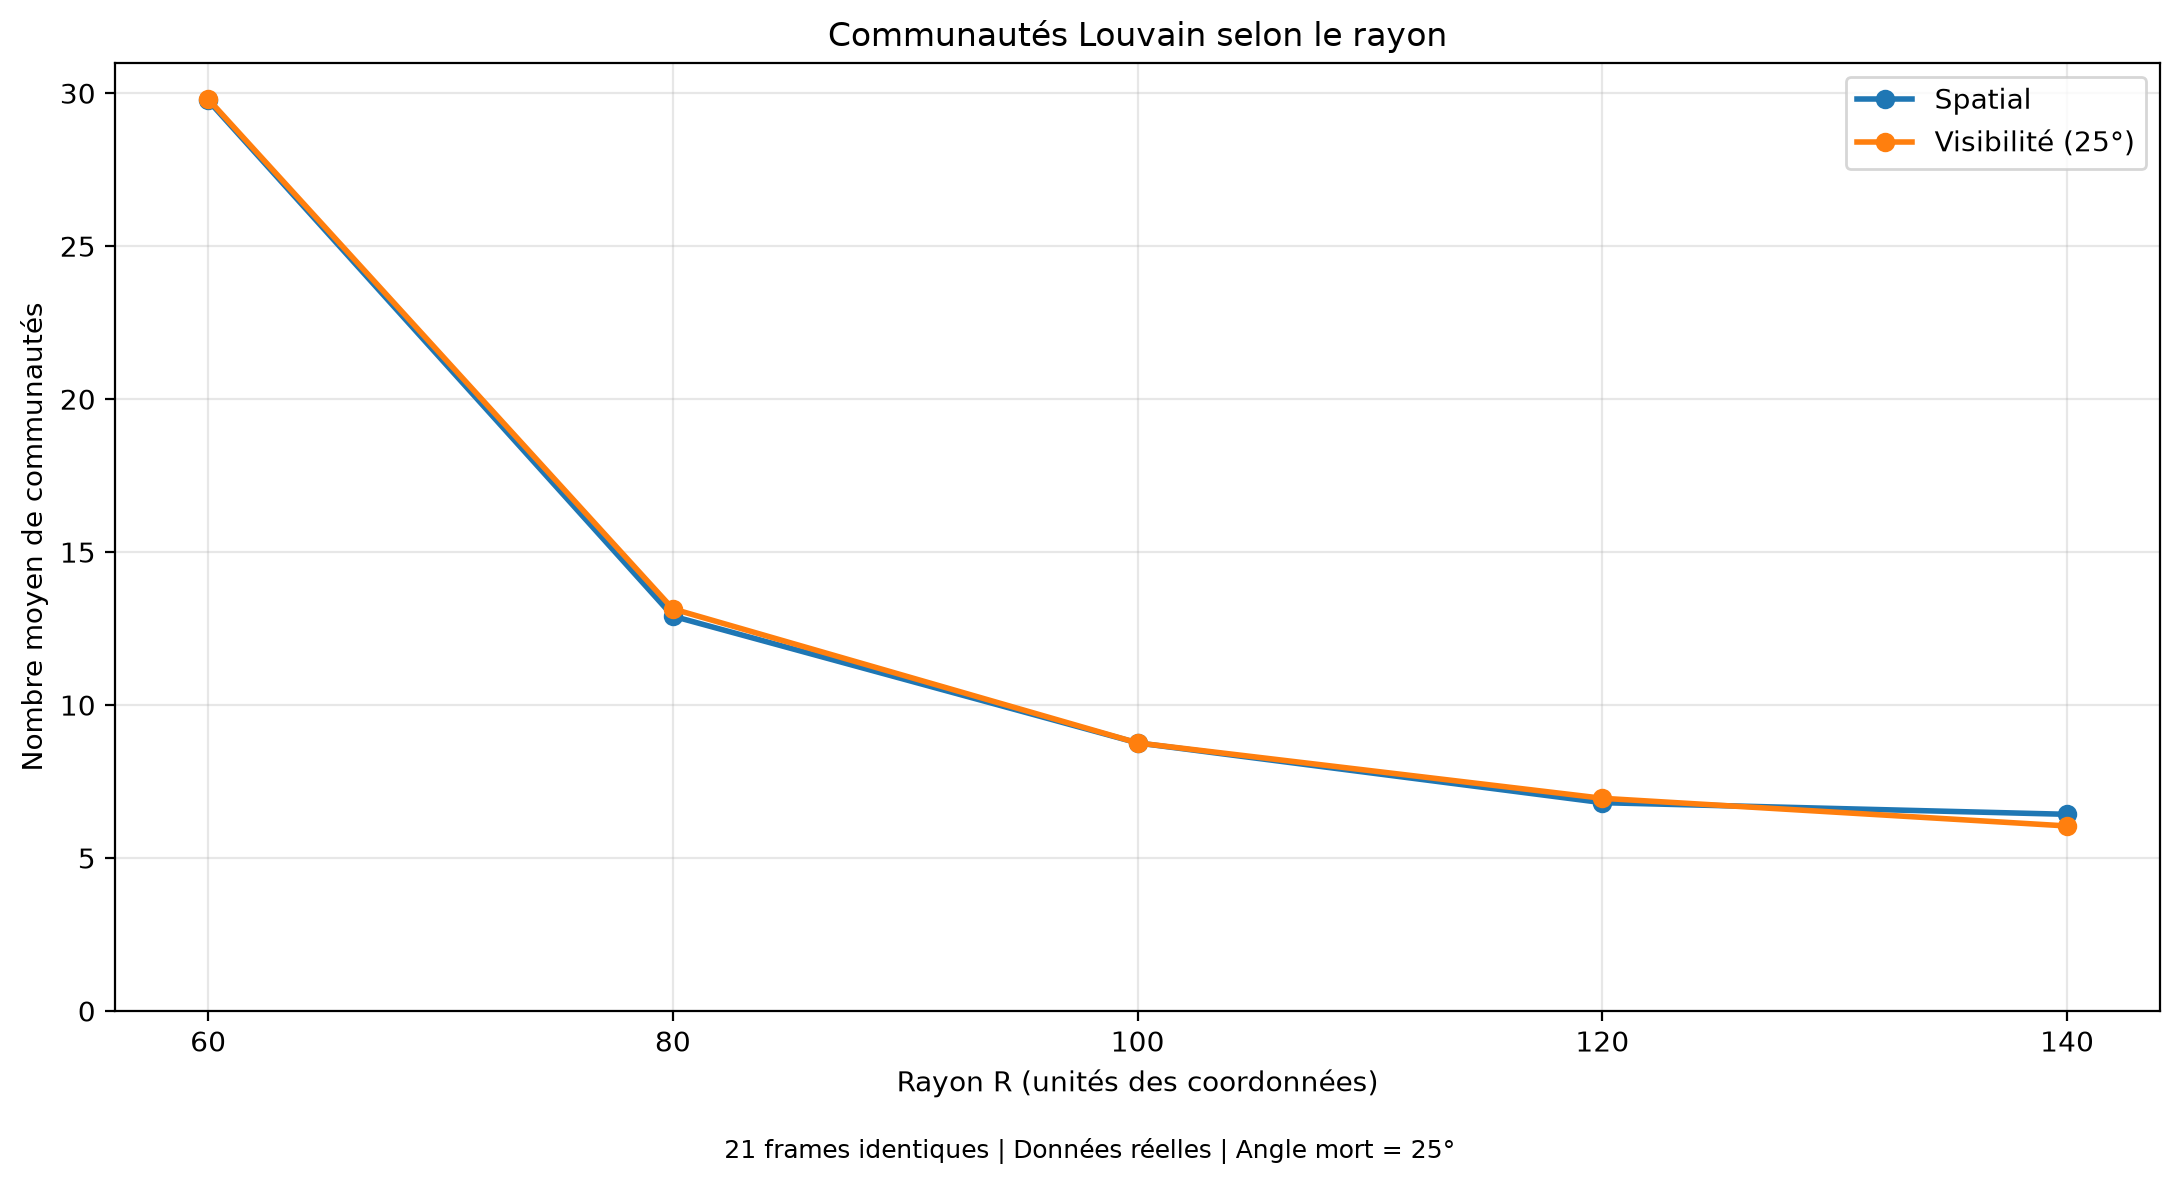
\includegraphics[width=\linewidth]
        {sensitivity_communities.png}
        \caption{Mean number of communities.}
        \label{fig:sensitivity_communities}
    \end{subfigure}

    \caption{Evolution of the mean
    clustering coefficient and the
    number of Louvain communities
    as a function of the
    neighbourhood radius.}

    \label{fig:sensitivity_clustering_communities}
\end{figure}

The mean clustering coefficient increases
from 0.41344 at $R=60$ to 0.63357
at $R=140$ in the spatial graph.

The visibility graph follows a similar
trajectory, with slightly lower
clustering values.

This increase indicates that larger
neighbourhood radii produce a greater
proportion of interconnected neighbours,
resulting in denser local structures.

Conversely, the mean number of detected
communities decreases as the
neighbourhood radius increases.

For the spatial graph, the mean number
of communities declines from 29.76
at $R=60$ to 6.43 at $R=140$.

A comparable evolution is observed
for the visibility graph.

At smaller radii, the network contains
numerous local groups, some of which
are disconnected or weakly connected
to the remaining structure.

As the radius increases, additional
connections emerge between these
groups, reducing the degree of
network fragmentation.

The simultaneous increase in clustering
and decrease in the number of communities
illustrates the substantial influence
of the interaction radius on the
organisation of the constructed network.

\paragraph{Sensitivity of Louvain modularity}

Figure~\ref{fig:sensitivity_modularity}
illustrates the evolution of mean
Louvain modularity for the five
selected neighbourhood radii.

\begin{figure}[htbp]
    \centering

    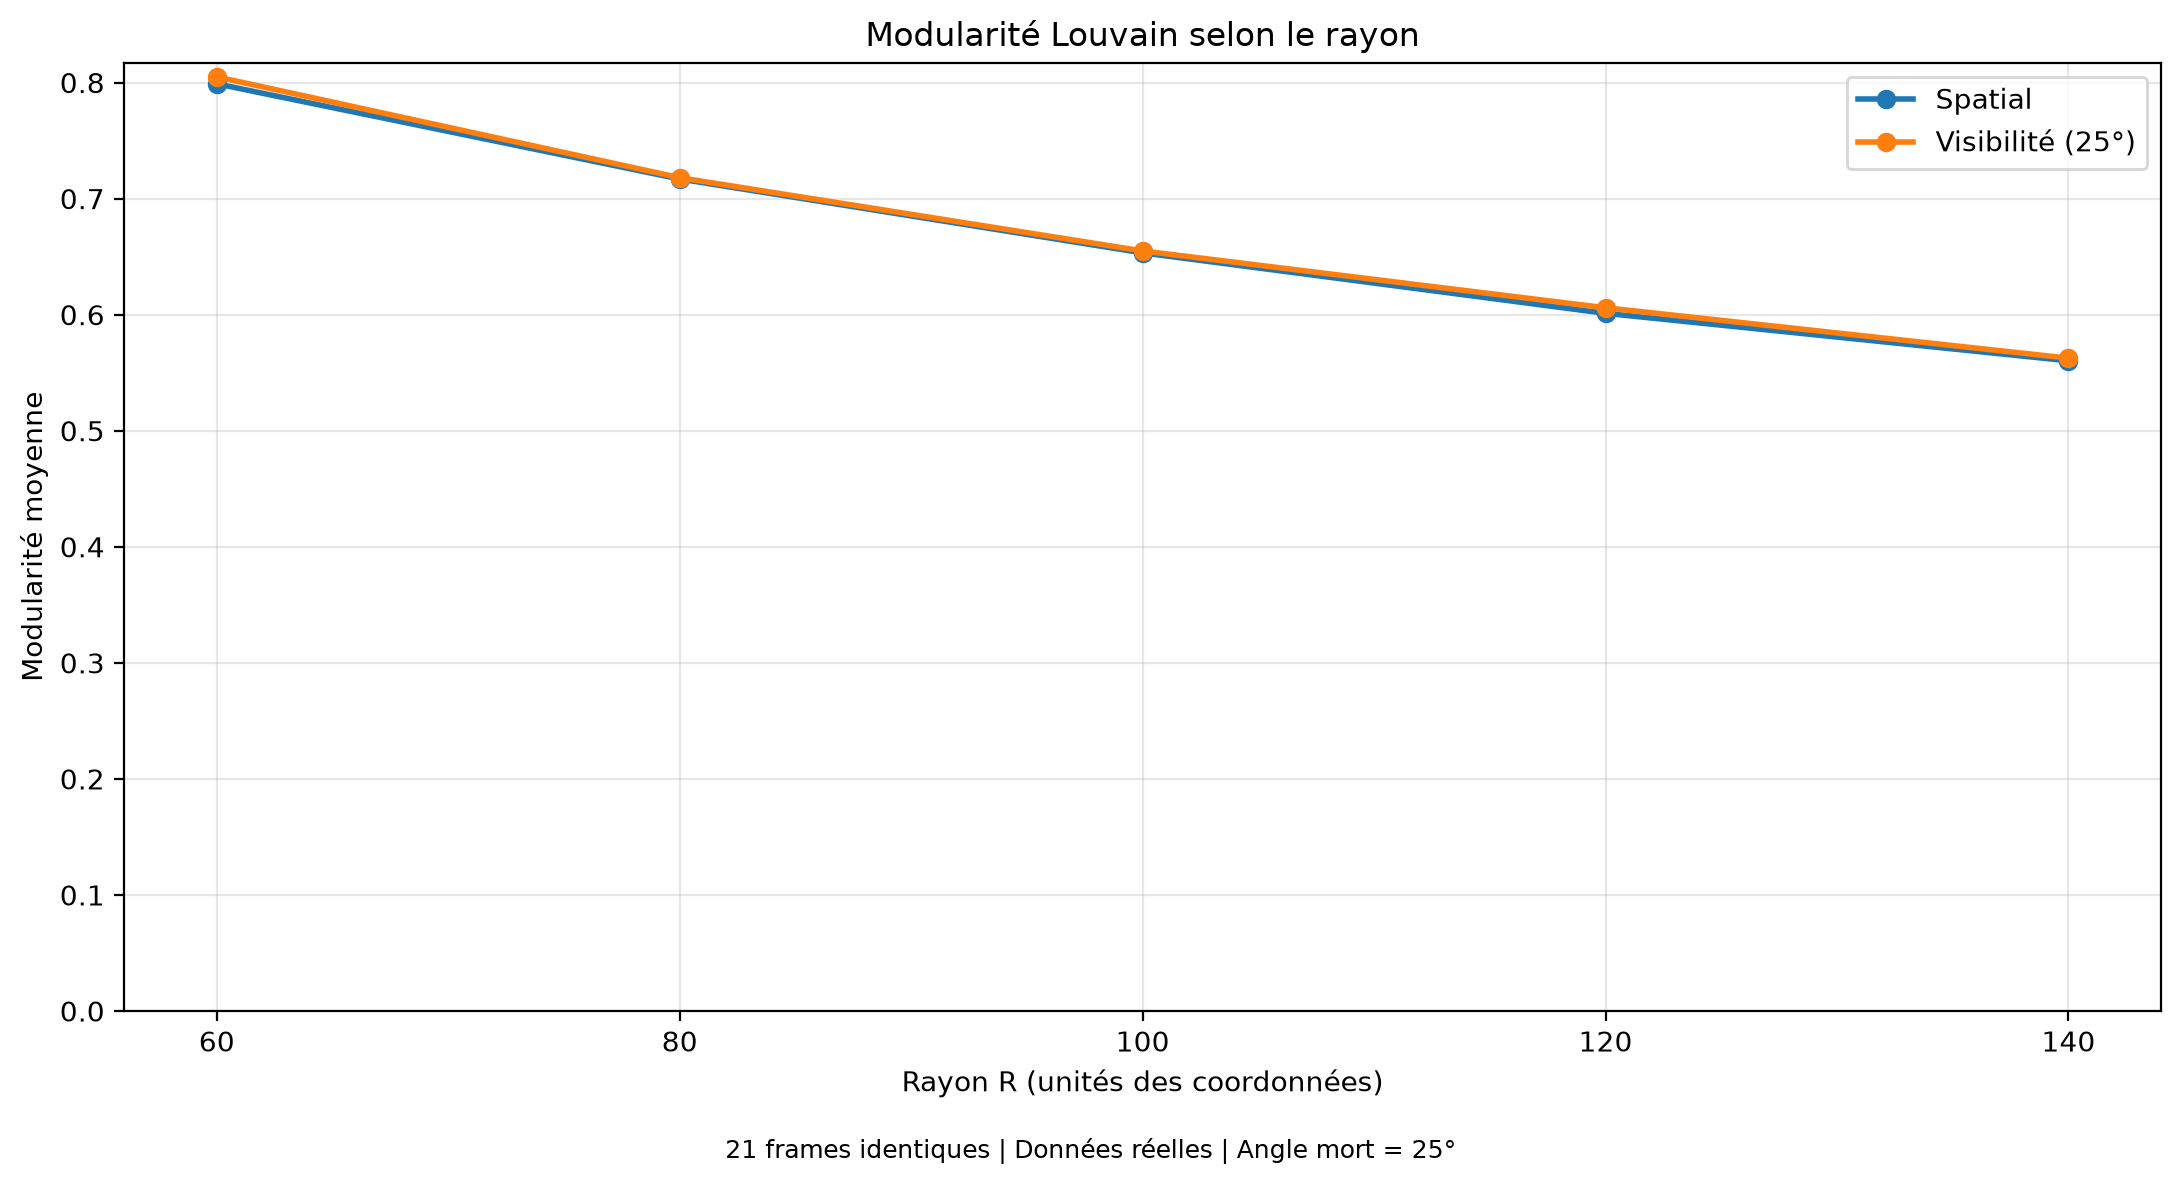
\includegraphics[width=0.78\textwidth]
    {sensitivity_modularity.png}

    \caption{Mean Louvain modularity
    as a function of the neighbourhood
    radius for the spatial and visibility
    networks, evaluated across
    21 identical experimental frames.}

    \label{fig:sensitivity_modularity}
\end{figure}

The mean modularity decreases
as the neighbourhood radius increases.

For both graph representations,
modularity is approximately 0.80
at $R=60$ and decreases to
approximately 0.56 at $R=140$.

The two curves remain particularly
close throughout the analysis,
indicating that the overall trend
is comparable between the spatial
and visibility models.

This decrease suggests that the
relative distinction between
detected communities becomes
less pronounced as the network
becomes increasingly connected.

At smaller radii, the graph
contains more clearly separated
local structures, producing
higher modularity values.

At larger radii, additional
connections between previously
distinct groups reduce their
relative separation.

Nevertheless, the modularity
values depend on the network
construction rule and the
community detection procedure.

They must therefore be interpreted
as structural properties of the
selected graph representations,
rather than direct measurements
of biological social organisation.

\paragraph{Interpretation of the reference radius}

The sensitivity analysis demonstrates
that the neighbourhood radius
substantially influences the
topological properties of the
constructed networks.

A smaller radius produces
sparser and more fragmented
graphs, while a larger radius
generates denser structures
with stronger global connectivity
and fewer detected communities.

The reference value $R=100$
provides a practical compromise
for the present analysis.

At this radius, the largest
connected component contains
more than 99\% of the observed
individuals on average, while
the network retains a differentiated
community structure.

However, this choice remains
a modelling assumption.

The present results do not
establish that $R=100$
corresponds to an optimal
biological interaction distance.

The sensitivity analysis
therefore provides an essential
means of distinguishing
relatively robust structural
observations from properties
induced by the selected
neighbourhood threshold.

\FloatBarrier

\subsection{Comparison of Spatial and Visibility Models}

At $R=100$, the two models exhibit
similar average structural properties
across the 21 selected frames.

The mean spatial density is 0.06095,
compared with 0.05682 for the directed
visibility graph.

The corresponding mean clustering
coefficients are 0.57873 and 0.54529.

The mean modularity values are
0.65325 and 0.65490, respectively.

The directional visibility constraint
therefore reduces the number of
available connections without producing
a complete reorganisation of the network
under the selected angular parameter.

On average, the visibility graph retains
approximately 93.22\% of the potential
directed connections between spatially
neighbouring fish.

This result is consistent with the
relatively narrow rear blind sector
considered in the model.

Nevertheless, the comparison must
take account of the differences
between directed and undirected
network measures.

In particular, the largest connected
component of the spatial graph and
the largest strongly connected
component of the visibility graph
do not represent identical
accessibility conditions.

% ============================================================
% 5. CONCLUSIONS
% ============================================================

\section{Conclusion}

The analysis of the fish school through
spatial proximity and directed visibility
graphs provides a mathematical description
of its collective organisation.

By representing each observed individual
as a vertex and defining connections
according to spatial and directional
criteria, it becomes possible to examine
the connectivity, distances, centrality
and community structure of the school.

The results obtained for the first
observation frame show that most
individuals belong to a common
connected structure.

At the same time, the identification
of several communities indicates
that a globally connected network
may contain relatively distinct
regions of local organisation.

The analysis of centrality measures
also reveals differences between
individuals having numerous direct
connections and those occupying
positions of relatively high
betweenness.

These differences provide useful
information about the topology
of the network, although they
cannot establish the existence
of behavioural leadership.

The temporal analysis indicates
that the structural properties
of the observed networks vary
throughout the experimental sequence.

However, the interpretation of
these variations must take into
account changes in the number
of detected individuals and
the dependence of the graph
on its construction parameters.

The sensitivity analysis confirms
the importance of the neighbourhood
radius.

Increasing this parameter produces
denser graphs, larger connected
components and a reduction in the
mean number of detected communities.

The reference radius of 100 native
coordinate units therefore provides
a useful basis for descriptive
comparisons, without constituting
a biologically validated threshold.

The directed visibility model
introduces an additional level
of representation by considering
the approximate orientation of
individual movements.

Under the selected rear blind
angle, its structural properties
remain relatively close to those
of the spatial graph.

The principal limitation of
the study lies in the distinction
between spatial proximity and
actual behavioural interactions.

The existence of a connection
between two individuals does
not demonstrate communication,
influence or causal dependence.

Likewise, the community
structure identified by the
algorithms may partly reflect
the geometrical properties
of the graph construction.

The present work therefore
demonstrates the relevance
of graph-theoretical methods
for describing the structural
organisation of a fish school,
while emphasising the need
for caution when translating
network measures into
biological interpretations.

Further investigations may
consider the temporal persistence
of individual connections,
alternative neighbourhood
definitions and comparisons
between observed trajectories
and simulated collective
behaviours.

\esp 

\paragraph{Code Availability and Reproducibility.}

The source code, graph construction and analysis scripts,
Boids simulation implementations, and available
experimental results are accessible through the
project's public GitHub repository:

\begin{center}
\url{https://github.com/Charles-Scannavino/Projet_Graph_Analytics}
\end{center}

The repository provides the implementation details
required to examine the graph construction methods,
network measures, community detection procedures,
and simulation experiments presented in this report.

\esp

\begin{thebibliography}{99}

\bibitem{dataset}
Oregon State University.
\textit{Fish Schooling Data Subset}.
Research dataset.
\url{https://doi.org/10.7267/zk51vq07c}.

\bibitem{networkx}
Hagberg, A. A., Schult, D. A., and Swart, P. J. (2008).
Exploring network structure, dynamics, and function
using NetworkX.
In \textit{Proceedings of the 7th Python in Science
Conference (SciPy 2008)}, pp. 11--15.

\bibitem{louvain}
Blondel, V. D., Guillaume, J.-L., Lambiotte, R.,
and Lefebvre, E. (2008).
Fast unfolding of communities in large networks.
\textit{Journal of Statistical Mechanics:
Theory and Experiment}, 2008(10), P10008.
\url{https://doi.org/10.1088/1742-5468/2008/10/P10008}.

\bibitem{reynolds}
Reynolds, C. W. (1987).
Flocks, herds and schools:
A distributed behavioral model.
\textit{ACM SIGGRAPH Computer Graphics},
21(4), 25--34.
\url{https://doi.org/10.1145/37402.37406}.

\bibitem{vicsek}
Vicsek, T., Czir\'ok, A., Ben-Jacob, E.,
Cohen, I., and Shochet, O. (1995).
Novel type of phase transition in a system
of self-driven particles.
\textit{Physical Review Letters},
75(6), 1226--1229.
\url{https://doi.org/10.1103/PhysRevLett.75.1226}.

\bibitem{couzin}
Couzin, I. D., Krause, J., Franks, N. R.,
and Levin, S. A. (2005).
Effective leadership and decision-making
in animal groups on the move.
\textit{Nature}, 433, 513--516.
\url{https://doi.org/10.1038/nature03236}.

\bibitem{cucker}
Cucker, F., and Smale, S. (2007).
Emergent behavior in flocks.
\textit{IEEE Transactions on Automatic Control},
52(5), 852--862.
\url{https://doi.org/10.1109/TAC.2007.895842}.

\bibitem{pita}
Pita, D., Moore, B. A., Tyrrell, L. P.,
and Fern\'andez-Juricic, E. (2015).
Vision in two cyprinid fish:
Implications for collective behavior.
\textit{PeerJ}, 3, e1113.
\url{https://doi.org/10.7717/peerj.1113}.

\end{thebibliography}


\clearpage

\appendix

% Titres des annexes dans la table des matières
\renewcommand{\thesection}{Annexe \Alph{section}}



% Titres des annexes dans le document
\titleformat{\section}
  {\normalfont\Large\bfseries}
 % {Annexe \thesection\ --}
 { \thesection\ --}
  {1.5em}
  {}

% Éviter de répéter "Annexe" dans le titre
%\titleformat{\section}
 % {\normalfont\Large\bfseries}
 % {\thesection\ --}
 % {0.5em}
 % {}

% Numérotation des annexes
%\renewcommand{\thesection}{Annexe \Alph{section}}

% Présentation des titres des annexes


% ============================================================
% APPENDIX A
% ============================================================
%\titleformat{\section}
%  {\normalfont\Large\bfseries}
%  {Annexe \thesection\ --}
%  {0.5em}
%  {}
\section{Fish-School Modelling and Objectives}
\label{app:fish-model}

\subsection{Existing Models of the Problem}

This problem has given rise to several types of modelling.

One of the most interesting lines of research is associated
with Giorgio Parisi and his team, whose work on complex
systems was recognised by the 2021 Nobel Prize in Physics.

The model considered here is based on an earlier approach,
which remains highly influential in the literature on
\textbf{collective intelligence and the dynamics of
distributed agents}: that of Craig Reynolds (1987).

\subsection{Continuous Model of Propagation and
Cohesion--Repulsion in a Fish School}

\noindent\textbf{Modelling of Individuals}

We consider a set of $N$ fish, each identified by an index
$i\in\{1,\ldots,N\}$, and characterised by a position
$X_i(t)\in\mathbb{R}^2$ and a velocity
$V_i(t)=\dot X_i(t)$.

The direction of movement is given by the angle

\[
D_i(t)=\operatorname{atan2}(v_i^y,v_i^x),
\]

so that

\[
V_i(t)=v_i
\bigl(\cos D_i(t),\sin D_i(t)\bigr).
\]

The collective behaviour of the school is described
by the dynamics

\[
\frac{dV_i}{dt}
=
F_{\mathrm{cohesion},i}
+
F_{\mathrm{repulsion},i}
+
F_{\mathrm{alignment},i}
+
F_{\mathrm{danger},i},
\]

where each term represents a local interaction.

\subsubsection*{The Three Fundamental Forces}

The collective motion of the fish school is
represented through three local interaction
mechanisms: cohesion, repulsion (separation),
and alignment.

Each mechanism operates within a potentially
different interaction radius.

For fish $i$, the corresponding neighbourhoods
are defined as

\[
\mathcal N_i^{(c)}
=
\left\{
j\neq i:
\|X_j-X_i\|<R_c
\right\},
\]

\[
\mathcal N_i^{(s)}
=
\left\{
j\neq i:
\|X_j-X_i\|<R_s
\right\},
\]

\[
\mathcal N_i^{(a)}
=
\left\{
j\neq i:
\|X_j-X_i\|<R_a
\right\}.
\]

Here, $R_c$, $R_s$, and $R_a$ denote the
cohesion, separation (repulsion), and
alignment radii, respectively.

The separation radius is assumed to be smaller
than the cohesion radius:

\[
R_s<R_c.
\]

No additional ordering between the alignment
radius and the other radii is required by
the theoretical formulation.

\paragraph{a) Cohesion.}

Each fish is attracted towards the local
centre of mass of neighbouring individuals.

The cohesion force is defined as

\[
F_{\mathrm{cohesion},i}
=
k_c
\left(
\bar X_i^{(c)}-X_i
\right),
\]

where

\[
\bar X_i^{(c)}
=
\frac{1}{|\mathcal N_i^{(c)}|}
\sum_{j\in\mathcal N_i^{(c)}}X_j.
\]

The parameter $k_c>0$ controls the intensity
of the cohesion force.

If the cohesion neighbourhood is empty,
the cohesion force is set to zero.

\paragraph{b) Repulsion (Separation).}

A short-range repulsive interaction prevents
fish from approaching one another too closely.

The repulsion force is defined as

\[
F_{\mathrm{repulsion},i}
=
-k_r
\sum_{j\in\mathcal N_i^{(s)}}
\frac{X_j-X_i}
{\|X_j-X_i\|^2+\varepsilon},
\]

where $k_r>0$ controls the strength of
repulsion and $\varepsilon>0$ prevents
division by zero.

The negative sign ensures that the force
points away from nearby individuals.

Only fish belonging to the separation
neighbourhood contribute to this force.

If no neighbour is present within $R_s$,
the repulsion force is zero.

\paragraph{c) Alignment.}

Each fish tends to adjust its velocity
towards the average velocity of its
alignment neighbours.

The alignment force is defined as

\[
F_{\mathrm{alignment},i}
=
k_a
\left(
\bar V_i^{(a)}-V_i
\right),
\]

where

\[
\bar V_i^{(a)}
=
\frac{1}{|\mathcal N_i^{(a)}|}
\sum_{j\in\mathcal N_i^{(a)}}V_j.
\]

The parameter $k_a>0$ controls the
intensity of velocity adjustment.

If the alignment neighbourhood is empty,
the alignment force is set to zero.

\paragraph{Combined dynamics.}

The three interactions contribute to the
continuous-time velocity dynamics:

\[
\frac{dV_i}{dt}
=
F_{\mathrm{cohesion},i}
+
F_{\mathrm{repulsion},i}
+
F_{\mathrm{alignment},i}
+
F_{\mathrm{danger},i}.
\]

The danger term represents an optional
external perturbation, described separately
in the following subsection.

The equations above provide a theoretical
description of collective motion. The
discrete-time Boids implementation used in
the experiments is described in Appendix B.

\subsubsection*{Danger Force and Directional Propagation}

A localised danger, such as a predator, obstacle, or sudden
noise, may be detected by a fish located at the edge of the
school, identified by the index $i_0$.

As an illustrative scenario, the detecting fish may initially
change its direction by $45^\circ$ in response to the threat.
This angular change is a prescribed behavioural assumption;
it is not directly imposed by the repulsive force below.

Let $X_{\mathrm{danger}}$ denote the position of the danger
source and $X_{i_0}$ the position of the detecting fish.
The repulsive force is defined as

\[
F_{\mathrm{danger},i_0}
=
-k_d
\frac{X_{\mathrm{danger}}-X_{i_0}}
{\|X_{\mathrm{danger}}-X_{i_0}\|+\varepsilon},
\qquad k_d>0,\quad\varepsilon>0.
\]

The negative sign ensures that the force points away from
the danger source. The parameter $k_d$ controls its strength,
while $\varepsilon$ prevents division by zero.

\paragraph{Propagation of the directional response.}

The initial change in direction may subsequently propagate
through neighbouring fish. A simplified continuous model is

\[
\frac{dD_i}{dt}
=
\lambda\,\operatorname{wrap}(D_{i-1}-D_i),
\qquad\lambda>0,
\]

where $D_i$ denotes the direction of fish $i$ and $D_{i-1}$
that of a fish responding earlier.

The index $i-1$ refers to a predecessor in an assumed
propagation sequence, not necessarily the preceding
tracking identifier in the dataset.

The operator $\operatorname{wrap}$ returns the shortest
signed angular difference in $[-\pi,\pi]$, and $\lambda$
controls the adjustment rate.

A corresponding discrete-time directional adjustment is

\[
D_i^{(t+1)}
=
D_i^{(t)}+
\alpha\,\operatorname{wrap}\!\left(
D_{i-1}^{(t)}-D_i^{(t)}\right),
\qquad 0<\alpha<1.
\]

This formulation illustrates how a local directional change
could spread through a school.

It is a theoretical mechanism, not an experimentally
validated model of escape-wave transmission in the
observed dataset.

% The image already contains its own caption.
\begin{figure}[htbp]
    \centering
    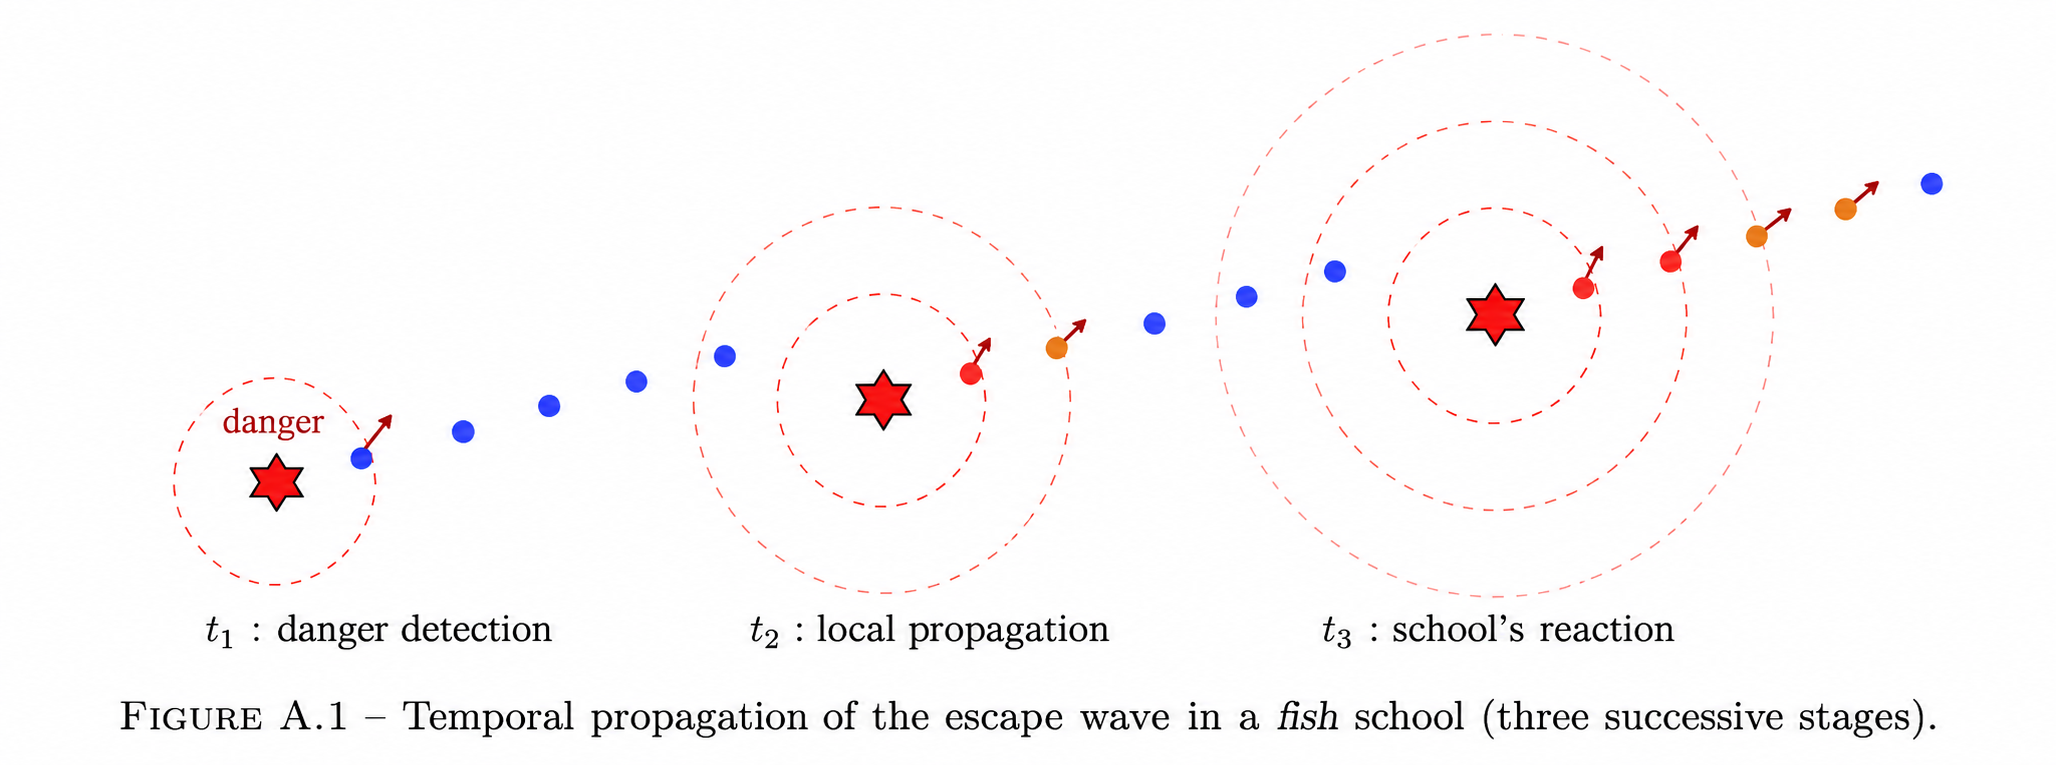
\includegraphics[width=0.94\linewidth]
    {danger_propagation.png}
\end{figure}

\subsection{Further Details on the Equations of Motion}

\subsubsection{Complete Equation of Motion}

The overall dynamics are written as

\[
\boxed{
\begin{aligned}
\frac{dX_i}{dt}
&=V_i,\\[4pt]
\frac{dV_i}{dt}
&=
k_c(\bar X_i-X_i)
-k_r\sum_{j\in\mathcal N_i}
\frac{X_j-X_i}
{\|X_j-X_i\|^2+\varepsilon}\\
&\quad
+k_a(\bar V_i-V_i)
+F_{\mathrm{danger},i}.
\end{aligned}
}
\]

This nonlinear coupled system is of the
\emph{agent-based continuous system} type.

Depending on its parameters and initial conditions,
it can produce collective motion, dispersion,
re-aggregation and changes in group organisation.

\subsubsection{Cohesion and Repulsion Mechanisms}

\begin{table}[htbp]
\centering
\small
\begin{tabular}{|l|l|l|l|}
\hline
\textbf{Interaction}
& \textbf{Range}
& \textbf{Formula}
& \textbf{Overall effect}\\
\hline
Cohesion
& $r<R_c$
& $k_c(\bar X_i-X_i)$
& Group maintenance\\
\hline
Repulsion
& $r<R_s<R_c$
& $-k_r(X_j-X_i)/r^2$
& Collision avoidance\\
\hline
Alignment
& $r<R_a$
& $k_a(\bar V_i-V_i)$
& Collective motion\\
\hline
Danger
& Localised
& $-k_d(X_{\mathrm{danger}}-X_i)/r$
& Escape response\\
\hline
\end{tabular}
\caption{
Local interactions, ranges of action and
their principal collective effects.
The simplified expressions in the table omit
regularisation terms.
}
\label{tab:app-forces}
\end{table}

These interactions are linearly superimposed
and integrated into the continuous dynamics,
giving rise to different forms of collective behaviour.

\subsection{Project Objectives}

\emph{Collective intelligence and the dynamics of
distributed agents} concern the ability of a set
of agents---individuals, animals, robots, etc.---
to produce coherent behaviour adapted to certain
situations in a decentralised manner,
without requiring a leader or central control.

Several hypotheses can therefore be considered
to obtain collective behaviours through dynamic
equations that can serve as a basis for simulation.

The resulting evolutions can then be compared
with collective movements recorded in a dataset.

The objective is to determine to what extent
local behavioural rules can reproduce the
spatial and structural organisation of an
experimentally observed fish school.

\esp

% ============================================================
% APPENDIX B
% ============================================================

\section{The Boids Model of Craig Reynolds (1987)}
%\label{app:boids}
%\titleformat{\section}
 % {\normalfont\Large\bfseries}
 % {Annexe \thesection\ --}
 % {0.5em}
%  {}

\subsection{General Introduction}

The \emph{boids} model (a portmanteau formed from
\emph{bird-oid object}) was proposed in 1987 by
Craig W. Reynolds in an article that has become
a classic:

\begin{quote}
Craig W. Reynolds,
``Flocks, Herds, and Schools:
A Distributed Behavioral Model'',
\emph{Computer Graphics
(SIGGRAPH '87 Conference Proceedings)},
Vol. 21, No. 4, pp. 25--34, 1987.
\end{quote}

It is a computational model of collective behaviour,
initially designed to simulate the flight of birds
or the movement of fish schools in three-dimensional
space.

This model is based on the idea that group coherence
does not require central coordination:
it emerges from simple local rules followed
by each agent.

\subsection{Fundamental Principle:
Local Behaviour, Global Emergence}

Each agent (or \emph{boid}) moves in a continuous
space, subject to three local behavioural rules:

\begin{enumerate}
    \item \textbf{Separation}:
    avoid collisions with immediate neighbours;

    \item \textbf{Alignment}:
    move in the same direction as nearby neighbours;

    \item \textbf{Cohesion}:
    move closer to the local centre of gravity
    of the group.
\end{enumerate}

Without any global command, these rules can produce
emergent collective behaviour:
swimming in formation, synchronised changes
in direction and the dynamic organisation
of a school.

\subsection{Mathematical Formalisation}

Let $N$ be the number of agents, each defined
by its position $X_i(t)\in\mathbb{R}^d$
and velocity $V_i(t)=\dot X_i(t)$,
with $d=2$ or $3$.

The temporal evolution of the system follows
the equation

\[
\frac{dV_i}{dt}
=
F_{\mathrm{separation},i}
+
F_{\mathrm{alignment},i}
+
F_{\mathrm{cohesion},i}
+
F_{\mathrm{other}},
\]

where $F_{\mathrm{other}}$ may include additional
forces such as obstacles, predators or goals
to be reached.

\paragraph{1. Separation (or repulsion).}

\[
F_{\mathrm{separation},i}
=
-k_s
\sum_{j\in\mathcal N_i^{(s)}}
\frac{X_j-X_i}
{\|X_j-X_i\|^2+\varepsilon}.
\]

Here, $\mathcal N_i^{(s)}$ is the set of neighbours
at a distance smaller than $R_s$.

This force pushes boid $i$ away from any neighbour
that is too close, preventing collisions and
maintaining a minimum distance.

\paragraph{2. Alignment.}

\[
F_{\mathrm{alignment},i}
=
k_a(\bar V_i-V_i),
\qquad
\bar V_i
=
\frac{1}{|\mathcal N_i^{(a)}|}
\sum_{j\in\mathcal N_i^{(a)}}V_j.
\]

Here, $\mathcal N_i^{(a)}$ denotes the neighbours
within a radius $R_a$.

The boid adjusts its velocity to the average
local velocity.

\paragraph{3. Cohesion (or attraction).}

\[
F_{\mathrm{cohesion},i}
=
k_c(\bar X_i-X_i),
\qquad
\bar X_i
=
\frac{1}{|\mathcal N_i^{(c)}|}
\sum_{j\in\mathcal N_i^{(c)}}X_j.
\]

This force attracts each boid towards the
centre of gravity of its neighbours within
a radius $R_c$.

\subsection{Mechanism of Emergence}

The three local rules, applied simultaneously
to each agent, can generate coherent and
dynamic collective structures:

\begin{itemize}
    \item Separation prevents internal collisions.
    \item Alignment promotes directional coherence.
    \item Cohesion maintains group compactness.
\end{itemize}

The global behaviours observed---formation,
avoidance and collective rotation---are
\emph{emergent phenomena}, rather than
behaviours explicitly specified in the model.

This approach illustrates the idea that
\emph{simple local rules} can generate
\emph{complex global patterns}.

\subsection{Extensions of the Model}

Since 1987, the boids model has undergone
numerous extensions:

\begin{enumerate}
    \item \textbf{Boids with limited perception}:
    introduction of a field of vision restricting
    interactions to visible neighbours.

    \item \textbf{Boids with inertia}:
    addition of inertial terms to velocities
    to simulate the physical continuity of movement.

    \item \textbf{Hierarchical boids}:
    leader or dominant agents orienting the group.

    \item \textbf{Environmental boids}:
    consideration of obstacles, currents or
    external potential fields.

    \item \textbf{Emotional or cognitive boids}:
    addition of internal variables such as
    stress, memory or goals.
\end{enumerate}

These variations make it possible to adapt
the model to different contexts:
biology, swarm robotics, three-dimensional
animation and crowd simulation.

\subsection{Relationship with Physical and
Biological Models}

The Reynolds model, although simple, is related
to several theoretical frameworks:

\begin{itemize}
    \item the dynamics of continuous multi-agent systems;
    \item mean-field equations used in statistical physics;
    \item biological models of local interaction
    (Cucker--Smale, Vicsek, Couzin et al.);
    \item self-organisation phenomena studied
    by Ilya Prigogine or Hermann Haken.
\end{itemize}

Thus, the boids model constitutes a bridge
between computer simulation and the theory
of complex systems.

\subsection{Equivalent Continuous Model}

In continuous form, the equation of motion
of a boid is written as

\[
\frac{dX_i}{dt}=V_i,
\]

\[
\begin{aligned}
\frac{dV_i}{dt}
&=
k_c(\bar X_i-X_i)
+k_a(\bar V_i-V_i)\\
&\quad
-k_s\sum_{j\in\mathcal N_i}
\frac{X_j-X_i}
{\|X_j-X_i\|^2+\varepsilon}.
\end{aligned}
\]

This nonlinear, self-regulated system
is simulated numerically by discrete integration.

\subsection{Extension: Radial Danger Field}

To incorporate escape behaviour in response
to a localised danger, an external field
$F_{\mathrm{danger}}$ centred at $X_0$
can be added.

One possible radial formulation is

\[
F_{\mathrm{danger},i}
=
k_d
e^{-\frac{\|X_i-X_0\|^2}{2\sigma^2}}
\frac{X_i-X_0}
{\|X_i-X_0\|+\varepsilon}.
\]

This field is intended to generate an outward
escape response when the school reacts to a
localised threat such as a predator.

The combination of internal forces and the
danger field may produce collective avoidance,
dispersion and subsequent realignment.

This extension remains a theoretical model;
it is not part of the calibrated experimental
comparison presented below.

\subsection{Qualitative Interpretation}

The boids model illustrates the transition
from the \emph{local to the global}:
group cohesion does not necessarily result
from central command, but can emerge from
distributed interactions.

It is a paradigmatic example of
\emph{emergent behaviour}.

\esp

% ============================================================
% APPENDIX C
% ============================================================

\section{Implementation and Visualisation
of the Fish School}
\label{app:implementation}

\subsection{Simulation Algorithm}

The simulation algorithm is based on
behavioural modelling of the Aoki (1982)
and Reynolds (1987) type.

Each fish interacts with nearby individuals
according to three principles:

\begin{enumerate}
    \item \textbf{Repulsion}:
    avoid collisions with fish that are too close;

    \item \textbf{Orientation}:
    align with the average direction
    of neighbouring individuals;

    \item \textbf{Attraction}:
    move closer to the local centre
    of the group to maintain cohesion.
\end{enumerate}

The simulated positions can then be represented
as a dynamic graph, allowing the comparison
of simulated and experimentally observed
spatial structures.

\subsection{Simulation of Behavioural Forces}

The Python implementation separates the
simulation of individual movement from
the construction and analysis of graphs.

The function \texttt{step\_boids()} applies
the local behavioural rules to update
the simulated positions and velocities.

Three fundamental forces are considered:
separation, alignment and cohesion.

The coefficients associated with these forces
determine their relative importance in the
resulting movement.

The implementation also provides an inertial
reference model through the function
\texttt{step\_persistence()}.

This reference model continues the movement
using the initial displacement, without
introducing the three behavioural interactions.

\subsection{Initialisation from Experimental Data}

The simulations are initialised using
experimentally observed positions from
the fish-school dataset.

Initial velocities are estimated from
consecutive observed positions.

This distinction is important because
the fields \texttt{vx} and \texttt{vy}
in the dataset represent directional information
and should not automatically be interpreted
as physical velocities expressed in
distance per unit of time.

The simulations therefore use the observed
displacements to initialise the predictive model.

\subsection{Management of Spatial Boundaries}

Spatial boundaries may be introduced in
a general fish-school simulation to represent
the walls of an aquarium.

In such a model, when a fish reaches
the limits

\[
(x_{\min},x_{\max},y_{\min},y_{\max}),
\]

its velocity can be reversed or corrected
to prevent it from leaving the simulation area.

This constitutes a possible boundary condition
for the theoretical model.

The experimental comparisons presented below
are instead interpreted through the numerical
simulation implemented in the project,
without attributing unverified physical
dimensions to the observation area.

\subsection{Animation of the Fish School}

Dynamic visualisation is produced using
the Python \texttt{matplotlib} library.

The graphical interface displays three
representations of the same group:

\begin{enumerate}
    \item the inertial reference simulation;
    \item the experimentally observed fish school;
    \item the interactive Boids simulation.
\end{enumerate}

The comparison is performed on a common
cohort of tracked fish, allowing their
positions and collective organisation
to be compared at the same prediction horizon.

\subsection{Analysis of Interindividual Distances
and Monitoring Graphs}

At each selected prediction horizon,
interindividual distances can be calculated
from the positions of the fish.

The distance to the nearest neighbour is

\[
d_i^{\mathrm{NN}}(t)
=
\min_{j\neq i}
\|X_i(t)-X_j(t)\|.
\]

The mean nearest-neighbour distance is

\[
\overline d_{\mathrm{NN}}(t)
=
\frac{1}{N}
\sum_{i=1}^{N}
d_i^{\mathrm{NN}}(t).
\]

These measurements provide indicators
of the spatial organisation of the school.

They can be compared between the observed
trajectories, the Boids simulation and
the inertial reference model.

\subsection{Visualisation of Collective Behaviour}

The program generates a dynamic representation
of the fish and their movement directions.

Fish positions are displayed graphically,
and their local relationships may be represented
using neighbourhood links.

The display evolves over time, allowing
the observation of directional alignment,
local dispersion and regrouping movements.

\subsection{Interactive Interface and User Control}
\label{app:interactive-interface}

An interactive graphical interface was developed
using Python, Matplotlib and
\texttt{matplotlib.widgets}.

It provides a visual environment for exploring
collective fish movement, adjusting simulation
parameters and comparing predictions with
experimental observations.

\subsubsection*{Organisation of the Interface}

The interface contains three synchronised
panels arranged horizontally:

\begin{itemize}
    \item \textbf{Inertia (left):}
    displays the inertial reference model,
    in which the initial movement is
    extrapolated without explicit
    behavioural interactions.

    \item \textbf{Real observations (centre):}
    displays the actual fish positions
    and movement directions extracted
    from the experimental dataset.

    \item \textbf{Interactive Boids (right):}
    displays the simulated trajectories
    obtained from the local rules of
    separation, alignment and cohesion.
\end{itemize}

All three panels use the same coordinate
system and the same cohort of tracked fish.
This arrangement allows the predicted
and observed spatial configurations
to be compared directly.

Fish are represented by triangular markers
oriented according to their direction
of movement.

The triangles therefore encode two
complementary properties:
the position of each fish and its
instantaneous movement direction.

When spatial edges are enabled,
lines connect fish belonging to the
same spatial neighbourhood, providing
a graphical representation of local
network connectivity.

\begin{figure}[htbp]
    \centering
    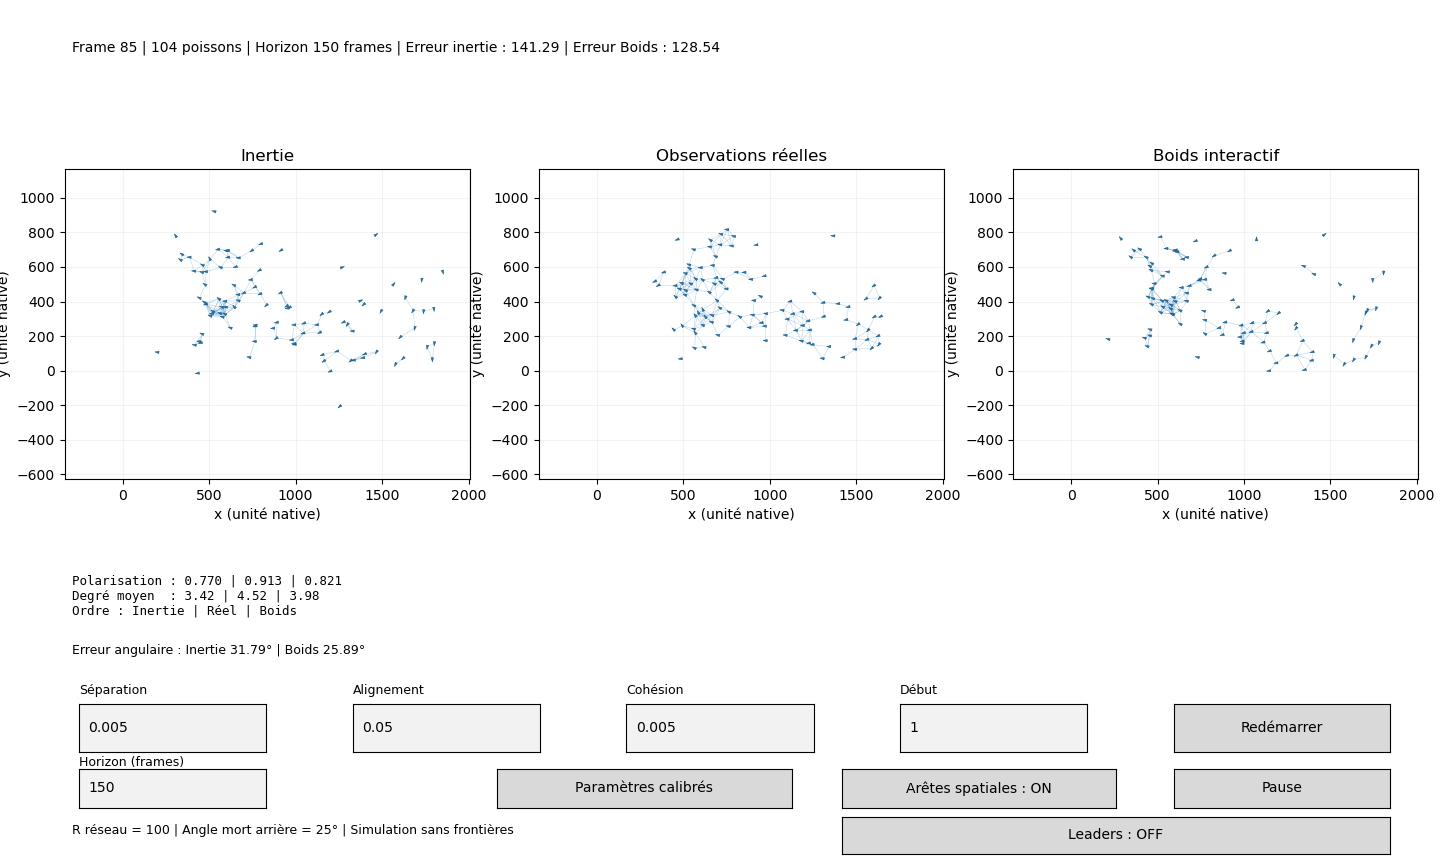
\includegraphics[
        width=\linewidth,
        keepaspectratio
    ]{Interface_Simulation.png}

    \caption{
    Interactive Matplotlib interface for
    comparing the inertial reference model
    (left), real fish observations (centre)
    and Boids simulation (right).
    Oriented triangular markers represent
    fish positions and movement directions.
    Spatial edges illustrate local
    neighbourhood relationships.
    The lower part of the interface contains
    simulation parameters, evaluation
    metrics and interactive controls.
    }

    \label{fig:boids-interactive-interface}
\end{figure}

\subsubsection*{Simulation Information}

The upper part of the interface displays
the current frame, the number of fish
included in the comparison and the
selected prediction horizon.

The displayed number of fish corresponds
to the cohort retained for the selected
simulation interval, rather than necessarily
to all fish detected in the original dataset.

The horizontal and vertical axes represent
the spatial coordinates of the fish
in native dataset units.

These coordinates are not interpreted
as physical distances in metres or
centimetres because their physical
calibration has not been established.

\subsubsection*{Quantitative Indicators}

The interface provides several indicators
for comparing the observed and simulated
collective behaviour.

\begin{itemize}

    \item \textbf{Position error:}
    measures the average distance between
    predicted and observed fish positions.
    Lower values indicate closer
    geometric agreement.

    \item \textbf{Angular error:}
    measures the average difference
    between predicted and observed
    movement directions, in degrees.
    Lower values indicate more accurate
    directional predictions.

    \item \textbf{Collective polarisation:}
    measures the degree of alignment
    of movement directions within
    the fish school.

    Its value ranges from 0 to 1,
    where values close to 1 indicate
    strongly aligned movement.

    \item \textbf{Mean graph degree:}
    represents the average number
    of spatial neighbours per fish
    in the corresponding graph.

    Higher values indicate a greater
    number of local connections,
    under the selected distance threshold.

\end{itemize}

The interface displays polarisation
and mean degree for the inertial,
observed and Boids configurations.

It also reports position and angular
errors for the two predictive models
relative to the real observations.

\subsubsection*{Illustrative Comparison}

Figure~\ref{fig:boids-interactive-interface}
shows an example at frame 85,
with 104 tracked fish and a
prediction horizon of 150 frames.

For this displayed state,
the position error is 141.29
for the inertial reference model
and 128.54 for the Boids simulation.

The corresponding angular errors
are 31.79 and 25.89 degrees,
respectively.

The displayed polarisation values
are 0.770 for inertia,
0.913 for the observations
and 0.821 for Boids.

The mean graph degrees are
3.42, 4.52 and 3.98,
respectively.

In this example, the Boids simulation
provides a smaller positional and
angular discrepancy than the
inertial reference model.

However, these values correspond
to a single displayed state.
They should not be interpreted
as evidence that Boids systematically
outperforms inertia over all
prediction horizons or observation windows.

The experimental validation
presented in Appendix D provides
a more systematic comparison.

\subsection{User Manual for the Visual Interface}

In the two-dimensional simulation model
developed in Python, several parameters
control the behaviour of the school
and the visualisation of its evolution.

These parameters modulate local interactions,
simulation duration and the display
of graph-related information.

\subsubsection*{Behavioural Parameters}

The interface provides editable fields
for the three main behavioural coefficients:

\begin{itemize}

    \item \textbf{Separation coefficient:}
    controls the intensity of the
    short-range repulsive force,
    which tends to prevent fish
    from approaching too closely.

    \item \textbf{Alignment coefficient:}
    governs the tendency of fish
    to adjust their movement directions
    towards those of neighbouring fish.

    \item \textbf{Cohesion coefficient:}
    controls the attraction of fish
    towards the local centre of
    their neighbourhood.

\end{itemize}

The theoretical model also defines
interaction radii for separation,
alignment and cohesion.

These radii determine which fish
are considered neighbours for
each behavioural interaction.

They should be distinguished from
the editable coefficients displayed
in the interface, which control
the strength of the corresponding forces.

\subsubsection*{Simulation Controls}

The graphical interface includes
the following interactive controls:

\begin{itemize}

    \item \textbf{Start frame:}
    selects the initial frame
    from which the simulation
    comparison is performed.

    \item \textbf{Prediction horizon:}
    determines the number of frames
    considered in the simulation.

    \item \textbf{Calibrated parameters:}
    applies a predefined configuration
    of behavioural coefficients obtained
    from the calibration procedure.

    \item \textbf{Restart:}
    reinitialises the simulation
    using the selected settings.

    \item \textbf{Pause:}
    temporarily stops the animation,
    allowing the current spatial
    configuration to be examined.

    \item \textbf{Spatial edges:}
    enables or disables the
    display of local graph connections.

    \item \textbf{Leaders:}
    enables or disables the display
    of potential leaders identified
    by the temporal analysis,
    when corresponding information
    is available.

\end{itemize}

The spatial graph is constructed
using a neighbourhood distance
threshold of $R=100$ in the
displayed configuration.

The interface also indicates
a rear blind angle of $25^\circ$,
associated with the visibility
modelling assumptions of the project.

The simulation shown in the
figure operates without
explicit spatial boundaries.

\subsubsection*{Execution of the Interface}

The graphical interface is implemented
in the Python module

\begin{verbatim}
src/boids_interface.py
\end{verbatim}

From the root directory of the
project repository, it can be
launched using:

\begin{verbatim}
python -m src.boids_interface
\end{verbatim}

The required Python dependencies
are listed in the repository's
\texttt{requirements.txt} file.

The original fish-school dataset
must also be available at the
location expected by the program.

\subsection{Graphical Analysis and Export}

The project produces numerical results
and graphical representations for several
prediction horizons.

The generated figures include comparisons
of spatial neighbourhoods, collective
polarisation, angular errors, mean degree
and nearest-neighbour distances.

These visualisations provide a complementary
interpretation of the numerical indicators.

The interactive interface additionally
allows the user to inspect the evolution
of the three models at corresponding
simulation frames.

It therefore connects the numerical
evaluation of predictive performance
with the visual interpretation of
collective movement and graph structure.

\subsection{Difficulties Encountered}

The experimental data introduce several
limitations for simulation and validation.

First, the number of detected fish varies
between frames.

Second, tracking identifiers do not guarantee
permanent biological identity throughout
the complete recording.

Third, the spatial coordinates are expressed
in native dataset units whose physical
calibration is not established.

Consequently, the simulation is evaluated
on cohorts of fish continuously observed
within the selected windows.

The results describe the performance
of a computational model under these
conditions, rather than a complete
biological reconstruction of fish behaviour.

\esp


% ============================================================
% APPENDIX D
% ============================================================

\section{Experimental Calibration and Validation
of the Boids Model}
\label{app:boids-validation}
%\titleformat{\section}
%  {\normalfont\Large\bfseries}
%  {Annexe \thesection\ --}
%  {0.5em}
%  {}

\subsection{Experimental Objective}

The purpose of the experimental analysis
is to evaluate whether the Boids model
can reproduce the observed movements
and spatial organisation of a fish school.

The simulations are compared with
the experimental trajectories using
a common initial state.

The main question is whether local rules
of separation, alignment and cohesion
provide a measurable improvement over
a simple inertial reference model.

\subsection{Experimental Dataset and Windows}

The experiments use the
\emph{Fish Schooling Data Subset}
from Oregon State University.

The dataset contains 5,000 frames
recorded at 30 frames per second.

For the predictive comparison,
three temporal windows are considered:

\begin{itemize}
    \item Frames 1--32:
    calibration and initial evaluation;

    \item Frames 2000--2031:
    independent validation;

    \item Frames 4000--4031:
    independent validation.
\end{itemize}

The simulations are initialised from
the first two observed positions.

Predictions are then evaluated at
horizons of 5, 10, 20 and 30 frames.

Only fish with continuous observations
throughout the corresponding window
are retained.

The resulting cohort sizes are
184 fish for the training window,
190 fish for the first validation window
and 232 fish for the second validation window.

\subsection{Inertial Reference Model}

The inertial model provides a baseline
against which the behavioural simulation
can be evaluated.

For each fish, the initial displacement
is estimated from two consecutive
observations:

\[
\widehat V_i(1)
=
X_i(2)-X_i(1).
\]

The subsequent position is predicted
by maintaining this displacement:

\[
\widehat X_i(t+1)
=
\widehat X_i(t)+\widehat V_i(1).
\]

This model does not include separation,
alignment or cohesion.

Its purpose is to determine whether
the introduction of local interactions
improves the prediction.

\subsection{Calibration of Behavioural Parameters}

The Boids model is controlled by
three principal coefficients:

\[
\theta=(k_s,k_a,k_c),
\]

where $k_s$, $k_a$ and $k_c$ correspond
respectively to separation, alignment
and cohesion.

A first calibration selected

\[
\boxed{
k_s=0,\qquad
k_a=0.15,\qquad
k_c=0.
}
\]

This configuration corresponds
to an alignment-only model.

A second optimisation explored
392 combinations of the three
behavioural coefficients.

The calibration was performed
on the training window only,
using the same spatial neighbourhood
radius

\[
R=100.
\]

Two optimisation objectives
were considered:

\begin{enumerate}
    \item maximising the mean spatial
    edge Jaccard similarity;

    \item minimising the position error
    at a prediction horizon of 30 frames.
\end{enumerate}

\subsection{Optimised Parameter Configurations}

The optimisation produced different
parameter configurations depending
on the evaluation criterion.

\begin{table}[htbp]
\centering
\small
\begin{tabular}{lccc}
\toprule
\textbf{Configuration}
& $k_s$ & $k_a$ & $k_c$\\
\midrule
Initial calibration
& 0 & 0.15 & 0\\
Best spatial Jaccard
& 0.005 & 0.05 & 0.005\\
Best position error
& 0.025 & 0.30 & 0.01\\
\bottomrule
\end{tabular}
\caption{
Behavioural coefficients selected
by the calibration procedures.
}
\label{tab:app-boids-parameters}
\end{table}

The results show that the preferred
combination depends on the objective.

The best configuration for reproducing
the graph structure is not necessarily
the best configuration for minimising
the geometric prediction error.

\subsection{Evaluation Metrics}

\subsubsection{Spatial Edge Jaccard Similarity}

The spatial graph is constructed
from the fish positions using
a distance threshold $R=100$.

For a given prediction horizon,
let $E_{\mathrm{real}}$
denote the set of observed edges
and $E_{\mathrm{sim}}$
the set of simulated edges.

The Jaccard similarity is

\[
J(E_{\mathrm{real}},E_{\mathrm{sim}})
=
\frac{
|E_{\mathrm{real}}\cap E_{\mathrm{sim}}|
}{
|E_{\mathrm{real}}\cup E_{\mathrm{sim}}|
}.
\]

A value close to 1 indicates
that the simulated and observed
graphs contain similar
neighbourhood relationships.

A value close to 0 indicates
limited overlap.

This measure evaluates structural
similarity rather than exact
geometric correspondence.

\subsubsection{Mean Position Error}

The mean position error is defined as

\[
E_{\mathrm{position}}(t)
=
\frac{1}{N}
\sum_{i=1}^{N}
\left\|
X_i^{\mathrm{sim}}(t)
-
X_i^{\mathrm{real}}(t)
\right\|.
\]

This metric measures the average
geometric difference between
simulated and observed positions.

The error is expressed in native
dataset units.

A smaller value indicates
a more accurate geometric prediction.

\subsubsection{Collective Polarisation}

Collective polarisation measures
the degree of directional alignment
within the school.

For the unit movement direction
$\widehat V_i(t)$ of each moving fish,

\[
P(t)
=
\left\|
\frac{1}{N}
\sum_{i=1}^{N}
\widehat V_i(t)
\right\|.
\]

A value close to 1 corresponds
to strongly aligned movement.

A value close to 0 corresponds
to weak overall directional coherence.

The difference between simulated
and observed polarisation provides
an additional measure of collective
behaviour.

\subsubsection{Mean Angular Error}

The angular difference between
the simulated and observed
movement directions is

\[
\theta_i(t)
=
\arccos
\left(
\frac{
V_i^{\mathrm{real}}(t)
\cdot
V_i^{\mathrm{sim}}(t)
}{
\|V_i^{\mathrm{real}}(t)\|
\|V_i^{\mathrm{sim}}(t)\|
}
\right).
\]

The mean angular error is

\[
E_{\mathrm{angular}}(t)
=
\frac{1}{N_{\mathrm{valid}}}
\sum_{i=1}^{N_{\mathrm{valid}}}
\theta_i(t).
\]

Only pairs with nonzero
movement vectors are considered.

The resulting angle is expressed
in degrees.

\subsubsection{Structural Graph Metrics}

Additional indicators are calculated
from the spatial graphs.

The mean degree is

\[
\overline k(t)
=
\frac{1}{N}
\sum_{i=1}^{N}k_i(t),
\]

where $k_i(t)$ denotes the
number of neighbours of fish $i$.

The nearest-neighbour distance
is also measured for each fish.

These metrics make it possible
to compare the simulated
local structure with the
experimentally observed structure.

\subsection{Validation on Independent Windows}

The selected parameter configurations
were evaluated on two temporal windows
not used during calibration.

At a prediction horizon of
30 frames, the following results
were obtained.

\begin{table}[htbp]
\centering
\small
\begin{tabular}{llcc}
\toprule
\textbf{Window}
& \textbf{Model}
& \textbf{Jaccard}
& \textbf{Position error}\\
\midrule
2000
& Inertia
& 0.5046 & 40.04\\
2000
& Initial calibration
& 0.5290 & 39.30\\
2000
& Jaccard-optimised
& 0.5182 & 39.28\\
2000
& Position-optimised
& 0.5321 & 38.09\\
\midrule
4000
& Inertia
& 0.5198 & 37.36\\
4000
& Initial calibration
& 0.5407 & 35.94\\
4000
& Jaccard-optimised
& 0.5458 & 35.54\\
4000
& Position-optimised
& 0.5384 & 35.91\\
\bottomrule
\end{tabular}
\caption{
Comparison of the inertial reference
and the calibrated Boids configurations
at a prediction horizon of 30 frames.
Position errors are expressed in
native dataset units.
}
\label{tab:app-boids-validation}
\end{table}

On the first validation window,
the position-optimised model
achieves a spatial Jaccard
similarity of 0.5321,
compared with 0.5046
for the inertial reference.

Its mean position error
is 38.09, compared with
40.04 for inertia.

On the second validation window,
the Jaccard-optimised model
achieves a spatial similarity
of 0.5458, compared with
0.5198 for inertia.

Its mean position error
is 35.54, compared with
37.36 for the inertial model.

\subsection{Interpretation of the Results}

The experimental results show
that local behavioural interactions
can improve the reproduction
of the observed fish-school structure
over the selected prediction horizons.

However, the improvement remains
relatively modest.

The results also reveal that
the calibration criterion matters:
a model optimised for spatial
connectivity does not necessarily
minimise the position error
on every validation window.

Furthermore, a configuration
selected during training does
not systematically outperform
all alternatives on unseen data.

These observations illustrate
the importance of evaluating
the simulation with several
complementary metrics.

\subsection{Experimental Limitations}

Several limitations must be considered
when interpreting the results.

First, the validation is based
on only two independent
temporal windows.

Second, the fish included
in each comparison are selected
according to the continuity
of their tracking identifiers
over the evaluation period.

Third, the physical scale
of the position coordinates
is not established.

Finally, the similarity
between observed and simulated
trajectories does not demonstrate
that the real fish follow
the Boids rules.

The results therefore support
a limited predictive comparison,
rather than a causal explanation
of biological collective behaviour.

\esp

% ============================================================
% APPENDIX E
% ============================================================

\section{Temporal Leadership Detection
and Collective Behaviour}
\label{app:leadership}
%\titleformat{\section}
%  {\normalfont\Large\bfseries}
%  {Annexe \thesection\ --}
%  {0.5em}
 % {}
\subsection{Leadership Hypotheses}

Several hypotheses may explain
the observed movements of a fish school:
erratic or genuinely random movements,
or movements dependent on certain
individuals whose directional changes
precede those of nearby fish.

These individuals might be located
at the front of the school,
at its centre or on its periphery,
where they may respond to
environmental changes.

Different collective trajectories
may therefore be obtained
from different hypotheses.

The relevance of each hypothesis
must ultimately be tested
by comparison with observed facts.

\subsection{Objective of the Temporal Analysis}

The purpose of the leadership analysis
is to identify individuals whose
directional changes systematically
precede similar changes
among neighbouring fish.

The analysis is based on
the temporal evolution of
the observed trajectories.

It does not assume that
the school possesses a permanent
leader or a centralised
decision-making structure.

Instead, leadership is treated
as a potential and measurable
temporal relationship.

\subsection{Construction of Turning Signals}

For each fish $i$,
the observed displacement
between two consecutive frames
is defined as

\[
V_i(t)
=
X_i(t+1)-X_i(t).
\]

The movement direction
is calculated using

\[
D_i(t)
=
\operatorname{atan2}
\left(
V_i^y(t),V_i^x(t)
\right).
\]

The angular variation
between consecutive
movement directions is

\[
\Delta D_i(t)
=
\operatorname{wrap}
\left(
D_i(t+1)-D_i(t)
\right),
\]

where the wrapping operation
returns the signed angular
difference in the interval

\[
[-\pi,\pi].
\]

This transformation makes
it possible to study
changes in direction
rather than absolute
positions alone.

\subsection{Temporal Correlation Between Fish}

To evaluate whether the
directional changes of fish $i$
precede those of fish $j$,
the turning signals are compared
with a temporal lag $\tau$.

The corresponding correlation is

\[
\rho_{ij}(\tau)
=
\operatorname{corr}
\left(
\Delta D_i(t),
\Delta D_j(t+\tau)
\right).
\]

Positive values of $\tau$
represent a situation in which
the turning signal of fish $i$
is compared with a later
turning signal of fish $j$.

The analysis considers
lags between 1 and 10 frames:

\[
\tau\in\{1,2,\ldots,10\}.
\]

At a recording frequency
of 30 frames per second,
this corresponds to delays
between approximately
0.033 and 0.333 seconds.

The strongest lagged correlation
is defined as

\[
\rho_{ij}^{\max}
=
\max_{\tau\in\{1,\ldots,10\}}
\rho_{ij}(\tau).
\]

\subsection{Identification of Potential Followers}

Two fish are considered
spatial neighbours when
their mean proximity
over a phase satisfies
the selected criterion.

The spatial distance
threshold is

\[
R=100.
\]

In the implementation,
a pair is retained when
the fish remain within
this distance for at least
half of the observations
in the corresponding phase.

A potential directional
relationship from fish $i$
to fish $j$ is retained
when the following
conditions are satisfied:

\[
\rho_{ij}^{\max}\geq 0.6,
\]

and

\[
\rho_{ij}^{\max}
-
\rho_{ij}(0)
\geq 0.1.
\]

The second condition
requires the lagged
correlation to exceed
the simultaneous
correlation by at least 0.1.

The implementation also
requires a minimum of
12 valid observation pairs
for the correlation
calculation.

These conditions reduce
the number of weak or
poorly supported
temporal associations.

They do not establish
causal influence.

\subsection{Influence Score}

For each fish $i$,
an influence score is
calculated from the
accepted lagged
correlations:

\[
I_i
=
\sum_{j\in\mathcal F_i}
\rho_{ij}^{\max},
\]

where $\mathcal F_i$
denotes the set of
potential followers
identified for fish $i$.

The number of followers is

\[
n_i^{\mathrm{followers}}
=
|\mathcal F_i|.
\]

An individual is classified
as a potential leader
during a phase when

\[
n_i^{\mathrm{followers}}\geq 2.
\]

This classification
is based on a numerical
criterion and should
not be interpreted as
proof of biological
leadership.

\subsection{Temporal Phases and Persistence}

The analysis is performed
on 150 consecutive frames
starting at frame 2000.

The observation period
is divided into five phases
of 30 frames each.

For each fish,
a binary indicator
$L_i^{(p)}$ is defined:

\[
L_i^{(p)}
=
\begin{cases}
1, & \text{if fish }i
\text{ is a potential leader in phase }p,\\
0, & \text{otherwise}.
\end{cases}
\]

The persistence score is

\[
P_i
=
\frac{1}{5}
\sum_{p=1}^{5}
L_i^{(p)}.
\]

A fish is considered
a persistent potential
leader when it is
classified as a leader
in at least three
of the five phases:

\[
\sum_{p=1}^{5}
L_i^{(p)}
\geq 3.
\]

This definition distinguishes
occasional temporal
precedence from repeated
identification across
several phases.

\subsection{Experimental Results}

The temporal analysis
identified several
individuals whose
directional changes
preceded those of
neighbouring fish
during particular phases.

The tracking identifier
105760 was classified
as a potential leader
in three of the five phases.

Its persistence score is

\[
P_{105760}
=
\frac{3}{5}
=
0.60.
\]

The corresponding
cumulative influence
score is approximately

\[
I_{105760}
=
5.7558.
\]

This individual is
therefore identified
as a persistent potential
leader under the
selected numerical criteria.

Other fish were identified
as potential leaders
in one or two phases,
indicating that temporal
precedence may vary
during the observation period.

\begin{table}[htbp]
\centering
\small
\begin{tabular}{lccc}
\toprule
\textbf{Fish ID}
& \textbf{Leader phases}
& \textbf{Persistence}
& \textbf{Total influence}\\
\midrule
105760 & 3 & 0.60 & 5.7558\\
104628 & 2 & 0.40 & 4.0692\\
105469 & 2 & 0.40 & 3.3261\\
105424 & 2 & 0.40 & 2.5783\\
105561 & 2 & 0.40 & 2.7288\\
\bottomrule
\end{tabular}
\caption{
Examples of potential leaders identified
by the temporal correlation analysis.
The identifiers correspond to tracking
labels within the selected observation
window.
}
\label{tab:app-leadership}
\end{table}

\subsection{Relationship with Graph Centrality}

The leadership analysis complements
the graph-theoretical study
presented in the main report.

Graph centrality measures
describe the structural position
of a node within a network.

For example, betweenness
centrality identifies nodes
located on a large proportion
of shortest paths.

However, structural centrality
and temporal leadership
are not equivalent concepts.

A fish may occupy a central
position in a proximity graph
without systematically
preceding the directional
changes of its neighbours.

Conversely, a fish may exhibit
temporal precedence
without being the most
central node in the network.

The two approaches therefore
provide complementary
descriptions of collective
organisation.

\subsection{Comparison with the Boids Model}

The Boids model is based
on decentralised local rules.

In its standard formulation,
no permanent leader
is required to coordinate
the group.

Nevertheless, some
individuals may temporarily
precede others in their
directional changes.

The temporal leadership
analysis therefore provides
an additional way to study
the organisation of
collective movement.

It may help distinguish
the existence of
temporary directional
precedence from
the stronger hypothesis
of permanent hierarchical
leadership.

The presence of a
temporally leading
individual does not
invalidate the possibility
of decentralised
collective behaviour.

\subsection{Limitations of Leadership Detection}

The interpretation of
the leadership results
requires several precautions.

First, a positive
lagged correlation
does not establish
a causal relationship.

Second, two fish may
react to the same
external stimulus
without one influencing
the other.

Third, the tracking
identifiers do not
guarantee permanent
biological identity
throughout the entire
dataset.

Fourth, the results
depend on the selected
distance threshold,
correlation threshold,
temporal lags and
phase duration.

Finally, the analysis
is performed on a
restricted observation
window.

The detected leaders
must therefore be
interpreted as
\emph{potential temporal
leaders}, rather than
confirmed biological
leaders.

\subsection{Interpretation of Collective Behaviour}

The results illustrate
the complexity of
collective organisation
within a fish school.

The movements of the
group may result from
local interactions,
temporary directional
precedence and changes
in spatial organisation.

The graph-theoretical
analysis describes
the structure of the
school, while the
temporal correlation
analysis examines
the ordering of
directional changes.

Together, these approaches
provide complementary
information about
collective dynamics.

They do not, however,
establish a unique
causal mechanism
responsible for the
observed movements.

\esp

% ============================================================
% APPENDIX F
% ============================================================

\section{General Discussion of the Simulation Extensions}
\label{app:bonus-discussion}
%\titleformat{\section}
%  {\normalfont\Large\bfseries}
%  {Annexe \thesection\ --}
%  {0.5em}
%  {}
\subsection{Relationship Between the Graph Models
and the Simulations}

The graph analysis
and the Boids simulations
address different
but complementary
aspects of the problem.

The spatial graph
describes the proximity
relationships between
fish at a given instant.

The directed visibility
graph introduces
an additional hypothesis
concerning the potential
perception of neighbouring
individuals.

The Boids model attempts
to reproduce the evolution
of positions using
local behavioural rules.

Finally, the leadership
analysis investigates
whether directional changes
of certain individuals
temporally precede those
of their neighbours.

These approaches
should not be confused.

A proximity edge
does not directly
represent a biological
interaction.

A visibility arc
does not demonstrate
that a fish is
actually attending
to another individual.

Likewise, a simulated
trajectory that resembles
an observed trajectory
does not establish
that the simulated
forces correspond
to the real biological
mechanisms.

\subsection{Principal Findings}

The experimental
comparisons show
that the calibrated
Boids models can
improve the prediction
of spatial relationships
and positions relative
to the inertial baseline
on the selected
validation windows.

However, the magnitude
of the improvement
is limited.

The optimisation also
shows that the choice
of evaluation criterion
influences the selected
behavioural parameters.

The temporal leadership
analysis identifies
individuals exhibiting
repeated directional
precedence, including
one tracking identifier
classified as a
persistent potential
leader in three
of five phases.

These findings provide
descriptive evidence
of heterogeneous
collective dynamics.

They do not demonstrate
the existence of
a permanent hierarchy
or a specific
biological mechanism.

\subsection{Perspectives}

Several extensions
could improve
the analysis.

A first possibility
would be to evaluate
the simulations
on a larger number
of independent
temporal windows.

A second would be
to investigate the
sensitivity of the
leadership results
to the selected
thresholds and lags.

A third would be
to compare additional
behavioural models
with the same
experimental trajectories.

Finally, a physical
calibration of the
spatial coordinates
would improve the
interpretability
of the distances
and interaction radii.

These developments
would provide a more
robust assessment
of the relationship
between local
behavioural rules
and observed
collective movement.

\esp

% ============================================================
% APPENDIX G
% ============================================================

\section{References for the Boids Model
and Collective Behaviour}
\label{app:bonus-references}

\begin{itemize}

% ------------------------------------------------------------
% Reynolds (1987) - Boids Model
% ------------------------------------------------------------

\item
Reynolds, C. W. (1987).
\emph{Flocks, Herds, and Schools:
A Distributed Behavioral Model}.
ACM SIGGRAPH Computer Graphics,
21(4), 25--34.

DOI:
\url{https://doi.org/10.1145/37402.37406}.

% ------------------------------------------------------------
% Parisi (2023) - Complexity and Collective Behaviour
% ------------------------------------------------------------

\item
Parisi, G. (2023).
\emph{Comme un vol d'\'etourneaux :
Une introduction personnelle
\`a la science de la complexit\'e}.
Flammarion.

French edition of
\emph{In un volo di storni}
(Rizzoli, 2021).

% ------------------------------------------------------------
% Vicsek et al. (1995) - Collective Motion
% ------------------------------------------------------------

\item
Vicsek, T., Czir\'ok, A.,
Ben-Jacob, E., Cohen, I.,
\& Shochet, O. (1995).
\emph{Novel type of phase transition
in a system of self-driven particles}.
Physical Review Letters,
75(6), 1226--1229.

DOI:
\url{https://doi.org/10.1103/PhysRevLett.75.1226}.

% ------------------------------------------------------------
% Couzin et al. (2005) - Collective Decision-Making
% ------------------------------------------------------------

\item
Couzin, I. D., Krause, J.,
Franks, N. R.,
\& Levin, S. A. (2005).
\emph{Effective leadership and
decision-making in animal groups on the move}.
Nature, 433(7025), 513--516.

DOI:
\url{https://doi.org/10.1038/nature03236}.

% ------------------------------------------------------------
% Cucker and Smale (2007) - Mathematical Flocking
% ------------------------------------------------------------

\item
Cucker, F., \& Smale, S. (2007).
\emph{Emergent behavior in flocks}.
IEEE Transactions on Automatic Control,
52(5), 852--862.

DOI:
\url{https://doi.org/10.1109/TAC.2007.895842}.

% ------------------------------------------------------------
% Pita et al. (2015) - Fish Vision
% ------------------------------------------------------------

\item
Pita, D., Moore, B. A.,
Tyrrell, L. P.,
\& Fern\'andez-Juricic, E. (2015).
\emph{Vision in two cyprinid fish:
implications for collective behavior}.
PeerJ, 3, e1113.

DOI:
\url{https://doi.org/10.7717/peerj.1113}.

% ------------------------------------------------------------
% Oregon State University - Fish Schooling Dataset
% ------------------------------------------------------------

\item
Oregon State University.
\emph{Fish Schooling Data Subset}.
Research dataset.

DOI (to be verified):
\url{https://doi.org/10.7267/zk51vq07c}.

\end{itemize}


% ============================================================
% APPENDIX H — SOFTWARE ARCHITECTURE AND PYTHON MODULES
% ============================================================

\section*{Appendix H -- Software Architecture and Python Modules}
\addcontentsline{toc}{section}{Appendix H -- Software Architecture and Python Modules}
\label{app:software_architecture}

\subsection*{H.1. General Architecture}

The project is implemented in Python and organised into
independent modules covering data processing, graph
construction, network analysis, numerical simulation,
visualisation and experimental validation.

The source code is publicly available at:

\begin{quote}
\texttt{github.com/Charles-Scannavino/Projet\_Graph\_Analytics}
\end{quote}

The repository separates the scientific analysis of
experimental fish-schooling networks from the complementary
Boids simulation and leadership analysis.

The main libraries include NumPy, SciPy, NetworkX,
Matplotlib and ijson. The pytest framework is used
for automated testing.

\subsection*{H.2. Data Loading and Graph Construction}

\begin{description}

\item[\texttt{data\_loader.py}]
Loads experimental observations from the JSON dataset.
It extracts fish identifiers, positions and velocity
components, and checks the structure of the input data.

\item[\texttt{graph\_builder.py}]
Constructs an undirected spatial proximity graph.
Each observed fish is represented by a vertex.
Two vertices are connected when their Euclidean
distance is smaller than the selected neighbourhood
radius. Distances are stored as edge attributes.

\item[\texttt{visibility\_graph.py}]
Constructs a directed visibility graph using spatial
proximity and an angular visibility constraint.
The reference configuration uses a total rear blind
sector of 25 degrees, with swimming direction
approximated from the recorded velocity vector.

\end{description}

\subsection*{H.3. Graph Analytics and Community Detection}

\begin{description}

\item[\texttt{graph\_metrics.py}]
Computes network characteristics, including graph
size, density, connected components, topological
distances and centrality measures.

\item[\texttt{community\_detection.py}]
Applies Louvain community detection to identify
groups of densely interconnected fish.
It produces community memberships and modularity
measurements.

\item[\texttt{temporal\_analysis.py}]
Constructs and analyses networks at selected
experimental frames. It measures changes in
network structure over time and exports the
corresponding numerical results.

\item[\texttt{sensitivity\_analysis.py}]
Studies the influence of the neighbourhood radius
on graph density, connectivity, clustering,
community structure and modularity.

\end{description}

\subsection*{H.4. Boids Simulation and Calibration}

The Boids extension investigates whether local
separation, alignment and cohesion rules can
reproduce observed collective motion.

\begin{description}

\item[\texttt{trajectory\_audit.py}]
Examines the continuity of tracked fish identifiers
and checks trajectory data quality across selected
experimental windows.

\item[\texttt{boids\_pilot.py}]
Implements the experimental Boids simulation
and compares predicted movements with a simple
inertial reference model.

\item[\texttt{boids\_behavior\_metrics.py}]
Provides behavioural indicators used to
characterise collective movement and compare
observed and simulated dynamics.

\item[\texttt{boids\_structural\_metrics.py}]
Provides graph-based structural indicators for
evaluating the spatial organisation of simulated
fish schools.

\item[\texttt{compare\_boids\_graphs.py}]
Compares experimental and simulated proximity
and visibility networks using structural metrics
and edge-set similarity.

\item[\texttt{calibrate\_boids.py}]
Explores combinations of behavioural coefficients
on the calibration window and selects a parameter
configuration according to the defined objective.

\item[\texttt{optimize\_boids\_weights.py}]
Provides an additional optimisation workflow
for the behavioural coefficients of the
simulation model.

\item[\texttt{validate\_boids\_windows.py}]
Evaluates simulation performance across several
experimental windows and prediction horizons.

\item[\texttt{validate\_calibrated\_boids.py}]
Evaluates calibrated parameters on independent
validation windows without repeating calibration.

\item[\texttt{validate\_optimized\_weights.py}]
Provides a validation workflow for the optimised
behavioural weights.

\item[\texttt{summarize\_boids\_validation.py}]
Consolidates experimental validation results
into summary tables for comparison and reporting.

\end{description}

\subsection*{H.5. Leadership Analysis}

\begin{description}

\item[\texttt{detect\_fish\_leaders.py}]
Implements the identification of potential
leaders from temporal fish movement data.

\item[\texttt{compare\_fish\_leadership.py}]
Compares leadership indicators and their
evolution across experimental configurations.

\item[\texttt{leader\_display.py}]
Provides visualisation utilities for displaying
potential leaders within the fish-school interface.

\end{description}

Leadership indicators are interpreted as exploratory
computational measures. They do not establish
biological leadership or causal influence.

\subsection*{H.6. Visualisation and Interactive Interface}

\begin{description}

\item[\texttt{visualize.py}]
Generates the reference spatial and visibility
network figures, including Louvain communities.
Fish are displayed using oriented markers based
on their recorded movement directions.
Figures are exported in PNG and SVG formats.

\item[\texttt{plot\_temporal.py}]
Produces figures illustrating the temporal
evolution of graph characteristics.

\item[\texttt{plot\_boids\_comparison.py}]
Generates comparative figures for experimental,
inertial and Boids simulation results.

\item[\texttt{boids\_interface.py}]
Implements the interactive graphical interface
used to inspect fish-school simulations.
It provides controls for behavioural parameters,
simulation playback and graph-related displays.

\end{description}

\subsection*{H.7. Automated Testing}

The repository contains a dedicated
\texttt{tests/} directory with automated tests.

The following test modules are included:

\begin{itemize}
    \item \texttt{test\_graph\_models.py}
    \item \texttt{test\_graph\_metrics.py}
    \item \texttt{test\_community\_detection.py}
    \item \texttt{test\_temporal\_analysis.py}
    \item \texttt{test\_sensitivity\_analysis.py}
    \item \texttt{test\_visualize.py}
    \item \texttt{test\_plot\_temporal.py}
    \item \texttt{test\_boids\_pilot.py}
    \item \texttt{test\_boids\_structural\_metrics.py}
    \item \texttt{test\_compare\_boids\_graphs.py}
    \item \texttt{test\_compare\_fish\_leadership.py}
    \item \texttt{test\_leader\_display.py}
\end{itemize}

These tests cover graph construction, network
metrics, community detection, temporal analysis,
simulation components and selected visualisation
functions.

The package also includes \texttt{src/\_\_init\_\_.py},
which identifies the source directory as a
Python package.

\subsection*{H.8. Execution and Reproducibility}

The project requires a compatible Python environment,
the dependencies listed in \texttt{requirements.txt},
and access to the original experimental dataset.

The dataset is expected at:

\begin{quote}
\texttt{data/schooling\_frames.json}
\end{quote}

The principal analyses can be reproduced from
the repository root using the following commands:

\begin{verbatim}
python -m src.graph_metrics
python -m src.community_detection
python -m src.visualize
python -m src.temporal_analysis
python -m src.plot_temporal
python -m src.sensitivity_analysis
\end{verbatim}

The interactive simulation can be launched using:

\begin{verbatim}
python -m src.boids_interface
\end{verbatim}

Automated tests can be executed using:

\begin{verbatim}
python -m pytest -q
\end{verbatim}

Generated outputs are stored under
\texttt{results/}, including numerical results,
experimental summaries and graphical figures.

The complete source code, execution instructions,
dependencies and available results are maintained
in the GitHub repository.

\subsection*{H.9. Scope and Scientific Reproducibility}

The modular implementation separates the
construction of experimental networks from
their analysis and from predictive simulation.

This separation makes it possible to examine
the effects of graph definitions, temporal
sampling and neighbourhood parameters without
confusing them with the assumptions of the
Boids model.

The original experimental observations remain
the reference data. Simulated trajectories
and derived network measures are interpreted
as computational approximations rather than
direct biological observations.

The repository provides the code required to
inspect the methodology and reproduce the
analyses, subject to the availability of the
original dataset and a compatible environment.


% ============================================================
% APPENDIX I — USE OF ARTIFICIAL INTELLIGENCE
% ============================================================

\section*{Appendix I -- Use of Artificial Intelligence}
\addcontentsline{toc}{section}{Appendix I -- Use of Artificial Intelligence}
\label{app:ai_usage}

Artificial Intelligence tools, primarily ChatGPT, were used
as supporting resources throughout the project, particularly
for Python programming assistance, debugging, code
documentation, and improving the clarity of technical
explanations.

AI assistance also helped explore possible analytical
approaches and organize the presentation of the results.
However, the research question, methodological choices,
graph construction parameters, and interpretation of the
findings remained under the responsibility of the students.

The generated suggestions were reviewed, adapted, and
checked against the dataset, Python implementations, and
experimental results. AI was therefore used as a
complementary development and learning tool, rather than
as a substitute for independent scientific reasoning and
critical analysis.

% ============================================================
% END OF APPENDICES
% ============================================================

\end{document}